\documentclass[a4paper]{article}
%% Language and font encodings
\usepackage[english]{babel}
\usepackage[utf8x]{inputenc}
\usepackage[T1]{fontenc}
\usepackage{float}
%% Sets page size and margins
\usepackage[a4paper,top=3cm,bottom=2cm,left=3cm,right=3cm,marginparwidth=1.75cm]{geometry}
\usepackage[caption=false]{subfig}
\setcounter{section}{-1}
%% Useful packages
\usepackage{fancyhdr}
\pagestyle{fancy}
\usepackage{tensor}
\usepackage{amsmath}
\usepackage{amsthm}
\usepackage{enumitem}
\usepackage{eqnarray}
\usepackage{float}
\usepackage{esint}
\usepackage{wrapfig}
\usepackage{gensymb}
\usepackage{lipsum}
\usepackage{amssymb}
\usepackage{array}
\usepackage{tikz}
\usetikzlibrary{arrows,decorations.markings}
\usepackage[colorlinks=true, allcolors=blue]{hyperref}
\usepackage{graphicx}
\usepackage{amsmath}
\usepackage{amssymb}
\usepackage{graphicx}
\usepackage{mathtools}
\usepackage[colorlinks=true, allcolors=blue]{hyperref}
\DeclareMathOperator{\lcm}{lcm}
\DeclareMathOperator{\var}{Var}
\DeclareMathOperator{\sech}{sech}
\DeclareMathOperator{\cosech}{cosech}
\DeclareMathOperator{\cov}{Cov}
\DeclareMathOperator{\sgn}{sgn}
\DeclareMathOperator{\Span}{span}
\DeclareMathOperator{\nullity}{nullity}
\DeclareMathOperator{\rank}{rank}
\DeclareMathOperator{\Ker}{Ker}
\DeclareMathOperator{\R}{R}
\DeclareMathOperator{\Tr}{Tr}
\DeclareMathOperator{\sinc}{sinc}
\DeclareMathOperator{\diag}{diag}
\newtheorem{remarks}{Remarks}[section]
\newtheorem{eg}{Example}[section]
\newtheorem{Note}{Note}[section]
\definecolor{darkblue}{RGB}{	0, 0, 139}
\newtheoremstyle{new}% <name>
{2pt}% <Space above>
{2pt}% <Space below>
{\color{darkblue}}% Body font
{}% <Indent amount>
{\bfseries\color{black}}% Theorem head font
{:}% <Punctuation after theorem head>
{.5em}% <Space after theorem headi>
{}% <Theorem head spec (can be left empty, meaning `normal')>
\theoremstyle{new}
\newtheorem{law}{Law}[section]
\newtheorem{defi}{Definition}[section]
\newtheorem{thm}{Theorem}[section]
\newtheorem{prop}{Proposition}[section]
\newtheorem{lemma}{Lemma}[section]
\newtheorem{cor}{Corollary}[section]

\title{\textbf{EO (Electrodynamics and Optics) Part II Phy}}
\author{Tai Yingzhe, Tommy (ytt26)}
\date{}
\setlength{\parindent}{0cm}
\begin{document}
\maketitle
{\small\tableofcontents}
%5 lectures from DAMTP electrodynamics, self read antenna and scattering and optics

\newpage
\section{Review of IB Electromagnetism}
\begin{defi}[Dielectric]
A dielectric material has no mobile charges that can move freely in an applied field but they nevertheless have a significant effect on applied electric fields. 
\end{defi}
\begin{defi}[Polarization]
The dipole moment per unit volume is called polarization $\mathbf{P}$.
\end{defi}
\begin{defi}[Electric Displacement]
We define the electric displacement to be
$$\mathbf{D}=\varepsilon_0\mathbf{E}+\mathbf{P}$$
\end{defi}
\begin{defi}[Linear Dielectric]
For linear dielectrics, the induced polarization $\mathbf{P}$ is proportional to the externally applied electric field $\mathbf{E}$.
\end{defi}
\begin{defi}[Electric Susceptibility]
The electric susceptibility is the constant of proportionality for the linear dielectric relation.
$$\mathbf{P}=\varepsilon_0\chi_e\mathbf{E}$$
\end{defi}
\begin{defi}[Permittivity and Dielectric Constant]
We define the permittivity of the material to be $\varepsilon:=\varepsilon_0(1+\chi_e)$ and $\varepsilon_r:=1+\chi_e$.
\end{defi}
\begin{cor}
In a linear dielectric, the displacement is also proportional to the field.
\end{cor}
\begin{proof}
$\mathbf{D}=\varepsilon_0\mathbf{E}+\mathbf{P}=\varepsilon_0(1+\chi_e)\mathbf{E}=\varepsilon\mathbf{E}$.
\end{proof}
\begin{defi}[Magnetic Material]
All materials are in some sense magnetic since they contain microscopic, atomic-scale currents and magnets which are themselves sources of magnetic field. When magnetically polarized, the material develops a magnetization.
\end{defi}
\begin{defi}[Magnetization]
Magnetization is the magnetic dipole moment per unit volume.
$$\mathbf{M}:=\frac{\boldsymbol{m}}{V}$$
\end{defi}
\begin{defi}[Auxiliary Field]
We define the auxiliary field to be
$$\mathbf{H}=\frac{1}{\mu_0}\mathbf{B}-\mathbf{M}$$
\end{defi}
\begin{defi}[Linear Magnetic Material]
For linear magnetic media, $\mathbf{M}$ is directly proportional to $\mathbf{H}$.
\end{defi}
\begin{defi}[Magnetic Susceptibility]
The magnetic susceptibility is the constant of proportionality for the linear magnetic media relation.
$$\mathbf{M}=\chi_m\mathbf{H}$$
\end{defi}
\begin{defi}[Relative Permeability]
We define the relative permeability $\mu_r:=1+\chi_m$.
\end{defi}
\begin{cor}
In a linear magnetic medium, the magnetic field is also proportional to the auxiliary field.
\end{cor}
\begin{proof}
$\mathbf{B}=\mu_0(\mathbf{H}+\mathbf{M})=\mu_0(1+\chi_m)\mathbf{H}=\mu\mathbf{H}$.
\end{proof}
\begin{Note}[Maxwell's Macroscopic Equations]
The Maxwell's equations in matter are:
$$\varepsilon_0\boldsymbol{\nabla}\cdot\mathbf{E}=\rho_f+\rho_b=\rho_f-\boldsymbol{\nabla}\cdot\mathbf{P}\implies\int_{\mathcal{S}}\mathbf{D}\cdot d\mathbf{S}=\int_{\mathcal{V}}\rho_fdV,\quad\boldsymbol{\nabla}\cdot\mathbf{D}=\rho_f$$
$$\int_{\mathcal{S}}\mathbf{B}\cdot d\mathbf{S}=0,\quad \boldsymbol{\nabla}\cdot\mathbf{H}=0$$
$$\oint_{\mathcal{C}}\mathbf{E}\cdot d\mathbf{l}=-\frac{d}{dt}\int_{\mathcal{S}}\mathbf{B}\cdot d\mathbf{S},\quad \boldsymbol{\nabla}\times\mathbf{E}=-\frac{\partial\mathbf{B}}{\partial t}$$
$$\frac{1}{\mu_0}\boldsymbol{\nabla}\times\mathbf{B}=\mathbf{J_f}+\mathbf{J_m}+\mathbf{J_b}+\varepsilon_0\frac{\partial\mathbf{E}}{\partial t}\implies\oint_{\mathcal{C}}\mathbf{H}\cdot d\mathbf{l}=\int_{\mathcal{S}}\mathbf{J_f}\cdot d\mathbf{S}+\frac{d}{dt}\int_{\mathcal{S}}\mathbf{D}\cdot d\mathbf{S},\quad\boldsymbol{\nabla}\times\mathbf{H}=\mathbf{J_f}+\frac{\partial\mathbf{D}}{\partial t}$$
\end{Note}
\begin{prop}[Statement of Conservation of Charge]
Consider a domain $D$ with boundary $S=\partial D$, the rate of change of charge density $\rho$ is related to the current density $\mathbf{J}$:
$$\frac{\partial\rho}{\partial t}+\boldsymbol{\nabla}\cdot\mathbf{J}=0$$
\end{prop}
\begin{prop}[Poisson's Equation]
The scalar electric potential $\phi$ satisfies the Poisson's equation, which is a linear PDE.
$$\nabla^2\phi=-\rho/\varepsilon_0$$
\end{prop}
\begin{prop}
The energy density of an electromagnetic field in a material is
$$u=\frac{1}{2}\mathbf{E}\cdot\mathbf{D}+\frac{1}{2}\mathbf{B}\cdot\mathbf{H}$$
The Poynting vector for these waves are $\mathbf{N}=\mathbf{E}\times\mathbf{H}$.
\end{prop}
\begin{prop}
The fields $\mathbf{E}$ and $\mathbf{B}$ can be written in terms of the potentials $\phi$ and $\mathbf{A}$. 
$$\mathbf{B}=\boldsymbol{\nabla}\times\mathbf{A},\quad\mathbf{E}=-\boldsymbol{\nabla}\phi-\frac{\partial\mathbf{A}}{\partial t}$$
These potential have gauge freedom.
\end{prop}
\begin{Note}[Boundary Conditions]
$$B_{\text{top}}^{\perp}=B_{\text{bottom}}^{\perp},\quad E_{\text{top},\parallel}=E_{\text{bottom},\parallel}$$
$$D_{\text{top}}^{\perp}-D_{\text{bottom}}^{\perp}=\sigma_f,\quad H_{\text{top}}^{\parallel}-H_{\text{bottom}}^{\parallel}=\mathbf{K_f}\times\mathbf{\hat{n}}$$
\end{Note}
\begin{prop}[Electromagnetic Waves]
The solution to Maxwell's equations in the case where $\rho=0$ and $\mathbf{J}=0$ (free space) is the equation of electromagnetic waves.
\end{prop}
\begin{remarks}\leavevmode
\begin{enumerate}
    \item Complex wavevector $\mathbf{k}+i\boldsymbol{\kappa}$ would mean the EM waves are damped. If $\mathbf{k}$ is parallel to $\boldsymbol{\kappa}$, the EM wave is homogeneous. Otherwise, it is inhomogeneous.
    \item The EM waves satisfy
    $$\mathbf{k}\cdot\mathbf{D}=0,\quad\mathbf{k}\cdot\mathbf{B}=0$$
    $$\mathbf{k}\times\mathbf{E}=\omega\mathbf{B},\quad\mathbf{k}\times\mathbf{H}=-\omega\mathbf{D}$$
    i.e. $\{\mathbf{B},\mathbf{k},\mathbf{E}\}$ and $\{\mathbf{D},\mathbf{k},\mathbf{H}\}$ are separately mutually orthogonal sets, while $\mathbf{E}$ and $\mathbf{H}$ are not necessarily perpendicular to $\mathbf{k}$. (It is, if the material is isotropic.)
\end{enumerate}
\end{remarks}
\begin{prop}
Some of the incident light on the interface of a linear media will be reflected and some will be transmitted. For s-polarization (light polarized in a direction perpendicular to the plane of incidence), the reflection and transmission ratios will be:
$$
r_s=\frac{\cos(\theta_i)-\sqrt{(\frac{n_t}{n_i})^2-\sin^2(\theta_i)}}{\cos(\theta_i)+\sqrt{(\frac{n_t}{n_i})^2-\sin^2(\theta_i)}},\quad t_s=\frac{2\cos(\theta_i)}{\cos(\theta_i)+\sqrt{(\frac{n_t}{n_i})^2-\sin^2(\theta_i)}}$$
For p-polarization (light polarized in a direction parallel to the plane of incidence), the reflection and transmission ratios will be:
$$
r_p=\frac{-(\frac{n_t}{n_i})^2\cos(\theta_i)+\sqrt{(\frac{n_t}{n_i})^2-\sin^2(\theta_i)}}{(\frac{n_t}{n_i})^2\cos(\theta_i)+\sqrt{(\frac{n_t}{n_i})^2-\sin^2(\theta_i)}},\quad t_p=\frac{2\cos(\theta_i)}{(\frac{n_t}{n_i})^2\cos(\theta_i)+\sqrt{(\frac{n_t}{n_i})^2-\sin^2(\theta_i)}}$$
\end{prop}
\begin{defi}[Brewster's angle]
The Brewster's angle is the angle of incidence where the reflection coefficient for light polarized parallel to the plane of incidence being zero.
\end{defi}
\begin{prop}[Plasma oscillations]
At the plasma frequency $\omega=\omega_p$, $\varepsilon(\omega_p)=0$, the wave is longitudinal with $\mathbf{k}$ parallel to $\mathbf{E}$.
\end{prop}
\newpage
\section{Optics}
\subsection{Polarization}
\begin{defi}[Linearly Polarized Waves]
A solution with real $\mathbf{E_0}$, $\mathbf{B_0}$, $\mathbf{k}$ is said to be linearly polarized.
\end{defi}
\begin{defi}[Elliptically Polarized Waves]
If $\mathbf{E_0}$ and $\mathbf{B_0}$ are complex, then it is said to be elliptically polarized.
\end{defi}
\begin{defi}[Circularly Polarized Waves]
For an elliptically polarized wave, if $|\boldsymbol{\alpha}| = |\boldsymbol{\beta}|$ and $\boldsymbol{\alpha}\cdot\boldsymbol{\beta}=0$, where $\mathbf{E_0}=\boldsymbol{\alpha}+i\boldsymbol{\beta}$.
\end{defi}
\begin{eg}
Take
$$\mathbf{E_T}=E_0(\mathbf{\hat{x}}e^{i(kz-\omega t)}+\mathbf{\hat{y}}e^{i(kz-(\omega t-0.5\pi))})$$
then $E_y$ lags behind $E_x$ by $\delta=\pi/2$. This is defined as a left-handed circularly polarized wave (LCP). An observer towards whom the light is propagating sees $\mathbf{E_T}(z=0)$ rotates anti-clockwise.
\end{eg}
\begin{eg}
For $|a_1|\neq|a_2|$ and $\delta\neq\pm\pi/2$, $\mathbf{E}$ is elliptically polarized with the major/minor axes along directions in the $xy$ plane determined as follows. With $a_1=a$, $a_2=be^{i\delta}$ such that $a,b\in\mathbb{R}$:
$$E_x=a\cos\omega t,\quad E_y=b\cos(\omega t-\delta)$$
which gives
$$\frac{E_y}{b}=\cos\omega t\cos\delta+\sin\omega t\sin\delta=\frac{E_x}{a}\cos\delta+\bigg(1-\frac{E_x^2}{a^2}\bigg)^{1/2}\sin\delta\implies\frac{E_x^2}{a^2}+\frac{E_y^2}{b^2}-2\cos\delta\frac{E_x}{a}\frac{E_y}{b}=\sin^2\delta$$
where $\alpha=0.5\tan^{-1}\frac{2ab\cos\delta}{a^2-b^2}$ is the angle the ellipse's axes are inclined to with respect to $E_x$ and $E_y$ directions.
\end{eg}
\begin{defi}[Jones Notation]
The complex amplitudes $a_1$ and $a_2$ of the two $x$ and $y$ linearly polarized waves can be used as the basis for a useful matrix approach for handling the effect of various optical devices on the polarization state.
\end{defi}
\begin{eg}
By definition, $x$- and $y$-polarized light are represented by $(1,0)$ and $(0,1)$ respectively, while $\theta$-polarized light is represented by $(\cos\theta,\sin\theta)$. Right circularly polarized and left circularly polarized light respectively represented by $(1/\sqrt{2})(1,-i)$ and $(1/\sqrt{2})(1,i)$. A general elliptically polarized light will be represented by $(a,be^{i\delta})$. Linear combinations, with appropriate phases, of the various polarization states can be used to form other polarization states. For instance, adding both RCP and LCP waves gives $x$-polarized waves.
\end{eg}
\subsection{Anisotropic Media}
\subsubsection{Dichroism}
\begin{defi}[Dichroic materials]
Dichroic materials absorb light linearly polarized in one direction more than light polarized in the other.
\end{defi}
\begin{eg}
A polaroid film is a plastic containing conducting polymeric chains aligned by stretching. If the sheet is anisotropic, conducting along $\mathbf{\hat{y}}$ but not along $\mathbf{\hat{x}}$, then light with $\mathbf{E}$ parallel to $\mathbf{\hat{y}}$ is absorbed while those parallel to $\mathbf{\hat{x}}$ is not. The Jones matrix representation for this polaroid is
$$J_x=\begin{pmatrix}1&0\\0&0\\\end{pmatrix}$$
In general, a polaroid with transmitting axis oriented at $\theta$ to $\mathbf{\hat{x}}$ is represented by
$$J_\theta=\begin{pmatrix}\cos^2\theta&\sin\theta\cos\theta\\\sin\theta\cos\theta&\sin^2\theta\\\end{pmatrix}$$
\end{eg}
\begin{eg}[Malus's Law]
For initially $x$-polarized light of intensity $I_0$ which then passes through polarizer $J_\theta$, the output is
$$J_\theta L_x=\begin{pmatrix}\cos^2\theta&\sin\theta\cos\theta\\\sin\theta\cos\theta&\sin^2\theta\\\end{pmatrix}\begin{pmatrix}1\\0\\\end{pmatrix}\sqrt{I_0}$$
so the transmitted intensity is
$$I(\theta)=I_0(\cos^4\theta+\sin^2\theta\cos^2\theta)=I_0\cos^2\theta$$
\end{eg}
\subsubsection{Birefringence}
\begin{defi}[Birefringence]
Birefringence is the optical property of a material having a refractive index that depends on the polarization and propagation direction of light. These optically anisotropic materials are said to be birefringent. It can be found from
$$\Delta n=n_e-n_o$$
where $n_e$ and $n_o$ are refractive indices along the extraordinary and ordinary ray.
\end{defi}
\begin{defi}[Permittivity/dielectric tensor]
For a materials with an anisotropic crystal structure, $\mathbf{E}$ is not necessarily parallel to $\mathbf{D}$ and we thus require a rank two tensor for permittivity, i.e.
$$D_i=\varepsilon_0\sum_j\varepsilon_{ij}E_j$$
\end{defi}
\begin{prop}
If the system has no energy loss, the dielectric tensor must be Hermitian.
\end{prop}
\begin{proof}
We have the rate of change of energy density in a material to be
$$\frac{du}{dt}=\frac{1}{2}\frac{d}{dt}(\mathbf{E}\cdot\mathbf{D}+\mathbf{B}\cdot\mathbf{H})=\frac{1}{2}(\mathbf{\dot{E}}\cdot\mathbf{D}+\mathbf{E}\cdot\mathbf{\dot{D}}+\mathbf{\dot{H}}\cdot\mathbf{B}+\mathbf{H}\cdot\mathbf{\dot{B}})$$
By Poynting theorem, this must be equal to $-\boldsymbol{\nabla}\cdot\mathbf{N}-\mathbf{J}\cdot\mathbf{E}$, but $\mathbf{N}=\mathbf{E}\times\mathbf{H}$ and the vector identity $\boldsymbol{\nabla}\cdot(\mathbf{a}\times\mathbf{b})=\mathbf{b}\cdot(\boldsymbol{\nabla}\times\mathbf{a})-\mathbf{a}\cdot(\boldsymbol{\nabla}\times\mathbf{b})$, hence by Maxwell equations,
$$\frac{du}{dt}=\mathbf{H}\cdot\mathbf{\dot{B}}+\mathbf{E}\cdot(\mathbf{J}+\mathbf{\dot{D}})-\mathbf{J}\cdot\mathbf{E}=\mathbf{H}\cdot\mathbf{\dot{B}}+\mathbf{E}\cdot\mathbf{\dot{D}}$$
Compare the first and last lines, we have
$$(\mathbf{\dot{E}}\cdot\mathbf{D}-\mathbf{E}\cdot\mathbf{\dot{D}})+(\mathbf{\dot{H}}\cdot\mathbf{B}-\mathbf{H}\cdot\mathbf{\dot{B}})=0$$
The dielectric and magnetic responses can usually be taken to be independent, so each of these bracketed terms must be zero. When $\mathbf{E}$ and $\mathbf{D}$ might be complex, it is necessary to take the real parts first
$$\text{Re}(\mathbf{E})\cdot\text{Re}(\mathbf{\dot{D}})=\text{Re}(\mathbf{D})\cdot\text{Re}(\mathbf{\dot{E}})$$
Assume $\mathbf{E}$ and $\mathbf{D}$ are varying time harmonically, then using 
$$\langle\text{Re}(a)\text{Re}(b)\rangle=\frac{1}{2}\text{Re}(a^*b),\quad a,b\in\mathbb{C}\implies\text{Re}(\mathbf{E^*}\cdot\mathbf{\dot{D}})=\text{Re}(\mathbf{\dot{E}})\cdot\text{Re}(\mathbf{D^*})$$
We then have $\varepsilon_{ij}=\varepsilon_{ji}^*$, i.e. Hermitian tensor.
\end{proof}
\begin{remarks}
For lossless media and in the absence of optical activity (see later), the dielectric tensor is real and hence symmetric. Thus, it can be diagonalized.
\end{remarks}
\begin{defi}[Principal refractive indices]
For a material with symmetric dielectric tensor, there is a set of orthogonal axes, known as the principal axes, such that we can cast the tensor as a diagonal matrix.
$$\varepsilon=\diag(\varepsilon_1,\varepsilon_2,\varepsilon_3)=\diag(n_1^2,n_2^2,n_3^2)$$
\end{defi}
\begin{defi}[Uniaxial and biaxial]
Materials with all three principal refractive indices being different is biaxial. If the material has two equal principal refractive indices, then it is uniaxial.
\end{defi}
\begin{eg}[Calcite]
Calcite (CaCO$_3$) is a naturally occurring mineral that crystallizes in a trigonal crystal structure. The crystal plane perpendicular to the optical axis has three-fold symmetry. The refractive index depends on the whether the direction of the electric field is in the plane of the triangular CO$_3$ clusters or perpendicular to them. Conventional to take $n_1=n_2\neq n_3$ for uniaxial system. Then, $n_3:=n_e$ where $e$ labels the extraordinary direction for the optic axis. We also have $n_1=n_2:=n_o$ for the ordinary direction. The birefringence for calcite is
$$\Delta n=n_e-n_o=-0.172$$
\end{eg}

\subsubsection{Linearly polarized EM waves in anisotropic media}
\begin{remarks}
For $\mathbf{D}$ to be parallel to $\mathbf{E}$, either
\begin{enumerate}
    \item $\mathbf{E}$ lies along one of the principal axes of a uniaxial or biaxial medium, or
    \item $\mathbf{E}$ is perpendicular to the optic axis of a uniaxial medium.
\end{enumerate}
If $\mathbf{E}\parallel\mathbf{D}$, then $\mathbf{E}\times\mathbf{H}=\mathbf{N}\parallel\mathbf{k}$, with wave velocity $c/n_{\mathbf{\hat{E}}}$ with refractive index along the direction whin $\mathbf{D}$ and $\mathbf{E}$ are directed. Otherwise, if this is not true, $\mathbf{N}$ may not necessarily be paralel to $\mathbf{k}$, i.e. the phas eand the energy may propagate in different directions.
\end{remarks}
\begin{defi}[Optical indicatrix]
With $\varepsilon_0\mathbf{D}\cdot\mathbf{E}=1$, we can define an ellipsoid
$$\mathbf{D}\cdot\varepsilon^{-1}\cdot\mathbf{D}=1\implies\frac{D_x^2}{\varepsilon_x}+\frac{D_y^2}{\varepsilon_y}+\frac{D_z^2}{\varepsilon_z}=1$$
called the optical indicatrix. For each polarization of $\mathbf{D}$, the corresponding $\mathbf{E}$ can easily be shown to be normal to the ellipsoid surface at the tip of $\mathbf{D}$.
\end{defi}
\begin{prop}
The length of the radius vector of the ellipsoid in each particulr direction equals the refractive index for a wave with polarization vector $\mathbf{D}$ in that direction.
\end{prop}
\begin{proof}
The refractive index experienced by a wave with polarization vector $\mathbf{D}$ is given by
$$n^2=\frac{c^2\mu_0D}{E\cos\alpha}=\frac{\varepsilon_0c^2\mu_0D^2}{\varepsilon_0ED\cos\alpha}=D^2$$
where $|\mathbf{k}\times\mathbf{k}\times\mathbf{E}|=k^2E\cos\alpha=\mu_0\omega^2D$ and $v^2=\omega^2/k^2$, and $\alpha$ is the angle between $\mathbf{E}$ and the plane perpendicular to $\mathbf{k}$.
\end{proof}
\begin{remarks}
In an anisotropic medium, it is the polarization direction $\mathbf{D}$, not the propagation direction that determines the wave velocity.
\end{remarks}
\begin{Note}[Huygens wavelets]
This can equivalently be represented in terms of the speed of Huygen's wavelets emanating from a point in the crystal and traveling in a particular propagation direction.
\begin{itemize}
    \item For wavelets with $\mathbf{D}$ perpendicular to the optic axis (without loss in generality, $z$-axis), the speed of the wavelet is $v_o=c/n_o$ and independent of their propagation direction. These are `ordinary' wavelets and form spherical wavefronts.
    \item For the linear polarizations orthogonal to the previous case, $\mathbf{D}$ lies in the $\mathbf{k_w}$-$\mathbf{\hat{e}_3}$ plane (where $\mathbf{k_w}$ is the wavevector of the wavelet) and in general $\mathbf{E}$ is not parallel to $\mathbf{D}$. The wavelet speed is $v_e=c/n_b$, where the effective refractive index $n_b$ is given by
    $$\frac{(n_b\sin\theta)^2}{n_e^2}+\frac{(n_b\cos\theta)^2}{n_o^2}=1$$
    where $\theta$ is the angle between the wavelet direction and $\mathbf{\hat{e}_3}$. These are `extraordinary' wavelets and form ellipsoidal wavefronts with cylindrical symmetry around $\mathbf{\hat{z}}$, since the velocity for points on the ellipsoidal wavefront is dependent on the polarization direction $\mathbf{D}$.
\end{itemize}
\end{Note}
\begin{eg}[Double refraction]
Consider linearly polarized light normally incident on a surface $S$ of a uniaxial crystal: $\mathbf{k_{inc}}$ is parallel to the surface normal $\mathbf{\hat{n}_S}$. Take the optic axis $\mathbf{\hat{e}_3}$ to be at an angle $\theta$ to $\mathbf{\hat{n}_3}$ in the plane of the figure. Inside the crystal, $\mathbf{k}$ is the wavevector for the transmitted ray formed from the superposition of many Huygens wavelets propagating in all directions. $\mathbf{k}$ is parallel to $\mathbf{\hat{n}_S}$ and so $\mathbf{k}$ makes an angle $\theta$ with $\mathbf{\hat{e}_3}$.
\begin{itemize}
    \item $\mathbf{D}\perp\mathbf{\hat{e}_3}$, $\mathbf{D}$ lies in the $\mathbf{\hat{e}_1}$-$\mathbf{\hat{e}_2}$ plane again, so $\mathbf{E}\parallel\mathbf{D}$ whatever its direction in this plane. The wavelets for the Huygen construction have speed $c/n_o$, independent of direction, and are therefore spherical and
    $$\mathbf{E}\times\mathbf{H}=\mathbf{N}\parallel\mathbf{k}$$
    This is the `ordinary' ray. At non-normal incidence, the ordinary ray would refract in the usual way in a medium with effective refractive index $n_o$.
    \item For the linear polarization orthogonal to the first case, $\mathbf{D}$ lies in the plane containing $\mathbf{\hat{e}_3}$, and in general $\mathbf{E}$ is not parallel to $\mathbf{D}$. The wavelet speed is $c/n_b$, and the Huygens wavelets are ellipsoidal. The tangent planes to the superposition of these ellipsoidal wavelets give the overall wavefronts for the propagating ray, and the direction of $\mathbf{k}$ for this ray remains normal to $S$. $\mathbf{D}$ is necessarily perpendicular to $\mathbf{k}$, but in general $\mathbf{E}$ is not parallel to $\mathbf{D}$, so $\mathbf{E}\times\mathbf{H}=\mathbf{N}$ is not parallel to $\mathbf{k}$. So while the phase again propagates along the surface normal $\mathbf{\hat{n}_S}$, the energy propagates at an angle to the normal: the `extraordinary' ray is therefore laterally shifted when it emerges from the crystal.
\end{itemize}
So an object viewed through a uniaxial crystal produces two images, one for the ordinary ray and one for the extraordinary ray - double refraction.
\end{eg}
\begin{eg}[Negative dielectric constant]
Some common metals such as Silver exhibit $\text{Re}[\varepsilon]=-2.4<0$. Imagine a multilayer structure of alternating layers from such a metal and a transparent dielectric with layer thickness $d_1$, $d_2$ and dielectric constants $\varepsilon_1<0$ and $\varepsilon_2>0$. This is an example of a metamaterial. Using the boundary conditions for the fields $\mathbf{D}$ and $\mathbf{E}$, we can calculate the effective dielectric constant for such a structure.
\begin{itemize}
    \item When the electric field is polarized parallel to the layers, $E_\parallel$ is conserved and the mean field $\overline{D}$ is the weighted mean of the fields $D=\varepsilon E$ in each of the layers
    $$\varepsilon_\parallel=\frac{\overline{D}}{E}=\frac{d_1\varepsilon_1+d_2\varepsilon_2}{d_1+d_2}$$
    On the other hand, when the electric field is polarized perpendicular to the layers, $D_\perp$ is conserved and
    $$\varepsilon_\perp=\frac{D}{\overline{E}}=\frac{d_1+d_2}{(d_1/\varepsilon_1)+(d_2/\varepsilon_2)}$$
\end{itemize}
If $\varepsilon_1\varepsilon_2<0$, then $(\varepsilon_1+\varepsilon_2)(\varepsilon_1^{-1}+\varepsilon_2^{-1})<0$, then in the range $|\varepsilon_1/\varepsilon_2|<d_{1,2}<|\varepsilon_2/\varepsilon_1|$, the effective dielectric constants satisfy
$$\varepsilon_{\parallel}\varepsilon_\perp<0$$
One such multilayer structure can be like alternating layers of Silver and a transparent dielectric Al$_2$O$_3$ with $\varepsilon_2=3.2$. This behaves like a uniaxial material with $\varepsilon_\parallel=+0.4$ and $\varepsilon_\perp=-9.6$. The optical indicatrix $\mathbf{D}\cdot\varepsilon\cdot\mathbf{E}=1$ is now a hyperboloid of one sheet:
$$\frac{D_x^2}{\varepsilon_\parallel}+\frac{D_y^2}{\varepsilon_\parallel}+\frac{D_z^2}{\varepsilon_\perp}=1$$
The refractive index surface is still a sphere for the ordinary waves, but becomes a hyperboloid of two sheets for the extraordinary waves. The two surfaces touch along the optical axis $\mathbf{\hat{z}}$.
\end{eg}
\newpage
\subsection{Optical Elements}
\begin{defi}[Waveplates]
A waveplate or retarder is an optical device that alters the polarization state of a light wave travelling through it. Two common types of waveplates are the half-wave plate, which shifts the polarization direction of linearly polarized light, and the quarter-wave plate, which converts linearly polarized light into circularly polarized light and vice versa. A quarter-wave plate can be used to produce elliptical polarization as well.
\end{defi}
\begin{eg}
Consider a waveplate such that the principal axes are along $\mathbf{\hat{x}}$, $\mathbf{\hat{y}}$ and $\mathbf{\hat{z}}$, with $n_x=n_f<n_y=n_s$, i.e. the $\mathbf{\hat{x}}$ and $\mathbf{\hat{y}}$ are the fast and slow axes respectively. A plane polarized EM wave $e^{i(kz-\omega t)}$ travels along $\mathbf{\hat{z}}$ at different speeds $c/n_f$ or $c/n_s$ depending on whether $\mathbf{E}$ is parallel to $\mathbf{\hat{x}}$ or $\mathbf{\hat{y}}$. The plate applies phase terms depending on the different optical thickness, i.e. $e^{i\omega nfd/c}$ and $e^{i\omega n_sd/c}$ to $L_x$ and $L_y$ respectively. So, the Jones matrix for the plate is
$$J_{\text{plate}}=\begin{pmatrix}e^{-i\Delta\phi/2}&0\\0&e^{i\Delta\phi/2}\\\end{pmatrix},\quad\Delta\phi=\omega\frac{d}{c}(n_s-n_f)$$
which is the phase difference induced by the plate for waves polarized along the fast and slow axes. For quarter-wave plate, $\Delta\phi=\pi/2\iff\lambda/4$ in vacuum, whereas for half-wave plate, $\Delta\phi=\pi\iff\lambda/2$ in vacuum.\\[5pt]
Suppose a plane polarized wave is incident on a wave plate (fast axis along $\mathbf{\hat{x}}$) with $\mathbf{E}$ at angle $\theta$ to $\mathbf{\hat{x}}$, i.e. incident wave represented by $(\cos\theta,\sin\theta)^T$, so the transmitted wave is $(e^{-i\Delta\phi/2}\cos\theta,e^{i\Delta\phi/2}\sin\theta)$. 
\begin{itemize}
    \item If $\Delta\phi=\pi/2$, we have an elliptically polarized light with $\alpha=0$, i.e. $(\cos\theta,i\sin\theta)$ with axes of ellipses lie along $\mathbf{\hat{x}}$ and $\mathbf{\hat{y}}$ have lengths $\cos\theta$ and $\sin\theta$. 
    \item If $\Delta\phi=\pi$, we have rotated plane polarized light. This time, with $\mathbf{E}$ directed at $-\theta$ to $\mathbf{\hat{x}}$.
\end{itemize}
\end{eg}
\subsection{Induced Birefringence}
\begin{defi}[Photoelasticity]
Photoelasticity (or stress birefringence) is the birefringence induced when an otherwise isotropic material is subjected to stress.
\end{defi}
\begin{defi}[Kerr Effect]
In an applied electric field $\mathbf{E_0}$ an otherwise isotropic material can become uniaxially birefringent, with the optic axis along $\mathbf{E_0}$. In liquids and gases, this can be understood as arising from the alignment of anisotropic molecules by the field. Since in an otherwise isotropic liquid or gas the optical properties cannot be sensitive to the sign of the field the change in the refractive index must be quadratic in the electric field to lowest order: $\Delta n=\lambda_0KE^2$ where $K$ is the Kerr constant. 
\end{defi}
\begin{defi}[Pockels Effect]
In solids a similar effect, the so-called Pockels effect, is associated with the lowering of the crystal symmetry by the induced macroscopic dielectric polarization. Crystals that do not have a centre of inversion symmetry could distinguish between positive and negative filds. Therefore, a linear electric field dependence is possible for the Pockels effect.
\end{defi}
Suitable materials can therefore be used to make voltage-controlled wave-plates.
\subsection{Optical Activity}
\subsubsection{Chiral materials}
\begin{defi}[Chiral]
A structure is chiral if it cannot be superposed on its mirror image by any combination of rotations and translations. Chiral materials are `optically active' and responds differently to LCP and RCP waves. These then are the natural polarization states to use - with two refractive indices $n_L$ and $n_R$.
\end{defi}
\begin{eg}
A chiral plate of thickness $d$ applies a phase term of $e^{i\omega n_{R,L}d/c}$ to the circularly polarized states accordingly. The relative phase is $\Delta\phi=\frac{\omega(n_L-n_R)d}{c}$, the linearly polarized waves (say in $x$-direction) become
$$\frac{1}{\sqrt{2}}\bigg[\frac{1}{\sqrt{2}}\begin{pmatrix}1\\-i\\\end{pmatrix}e^{-i\Delta\phi/2}+\frac{1}{\sqrt{2}}\begin{pmatrix}1\\i\\\end{pmatrix}e^{i\Delta\phi/2}\bigg]=\begin{pmatrix}\cos\Delta\phi/2\\-\sin\Delta\phi/2\\\end{pmatrix}$$
This is another plane polarized wave, but with its plane rotated clockwise by $\Delta\phi/2=\frac{\omega(n_L-n_R)d}{2c}$. The rotation per unit length - the specific rotatory power is $\alpha=\frac{\pi(n_L-n_R)}{\lambda}$.
\end{eg}
\begin{defi}[Dextrorotatory, levorotatory]
If the plane of polarization has rotated clockwise ($\alpha>0$, $n_L>n_R$), the medium is said to be dextrorotatory. If anti-clockwise ($\alpha<0$, $n_L<n_R$), the medium is said to be levorotatory.
\end{defi}
\subsubsection{Faraday effect}
\begin{defi}[Faraday effect]
Chirality may be induced in an isotropic medium by an application of a magnetic field. This is the Faraday effect. Compared to optically active media, the medium is now not optically isotropic.
\end{defi}
\begin{defi}[Faraday geometry]
Faraday geometry occurs when EM waves with $\mathbf{k}\parallel\mathbf{\hat{B}}$ in a plasma.
\end{defi}
\begin{defi}[Verdet coefficient]
The Verdet coefficient $V$ is defined to satisfy $\theta=VB_0d$ where $B_0$ is the magnitude of the $B$ field, $\theta$ is the rotation angle for the polarization plane after passing through a distance $d$ in the induced chiral material (via Faraday effect).
\end{defi}
\begin{prop}
The Verdet coefficient in a weak field $B_0$ for circularly polarized wave is
$$V=-\frac{e\omega_p^2}{2mc\omega^2\sqrt{1-\frac{\omega_p^2}{\omega^2}}}$$
\end{prop}
\begin{proof}
For each electron, the equation of motion is (neglecting any scattering and the negligible effect of the magnetic field of the EM wave):
$$m\mathbf{\ddot{r}}=-e(\mathbf{E}+\mathbf{\dot{r}}\times\mathbf{B_0})$$
where $\mathbf{E}=(E_x,E_y)^Te^{-i\omega t}$ is the electric field of the incident EM wave. Consider $\mathbf{r}=(x_0,y_0)^Te^{-i\omega t}$, then we have the equation of motion to simplify to
$$-\omega^2(x_0\pm iy_0)=-\frac{e}{m}(E_x\pm iE_y)\pm\omega\omega_c(x_0\pm iy_0)$$
Further simplify for circularly polarized wave, say LCP $E(1,i)^T$, then we have the circular polarization to be $P=-ena(1,i)^T=\varepsilon_0\chi_LE(1,i)^T$, where the effective susceptibility is 
$$\chi_L=-\frac{\omega_p^2}{\omega^2-\omega\omega_c}$$
where $\omega_p=ne^2/\varepsilon_0m$ is the plasma frequency. Similarly, for RCP, $\chi_R=-\frac{\omega_p^2}{\omega^2+\omega\omega_c}$. The dielectric constant will then be
$$\varepsilon_{L,R}(\omega)=1-\frac{\omega_p^2}{\omega(\omega\mp\omega_c)}$$
The plane of polarization of a plane polarized wave is steadily rotated as it passes through the optic axes of this material. The angle of rotation is
$$\theta=\frac{1}{2}\Delta\phi=\frac{\omega d}{2c}(n_L-n_R)=\frac{\omega d}{2c}\bigg[\sqrt{1-\frac{\omega_p^2}{\omega(\omega-\omega_c)}}-\sqrt{1-\frac{\omega_p^2}{\omega(\omega+\omega_c)}}\bigg]\approx-\frac{\omega_p^2\omega_cd}{2c\omega^2\sqrt{1-(\omega_p/\omega)^2}}$$
where $\omega_c,B_0<<1$.
\end{proof}
\begin{prop}
The dielectric tensor for Faraday geometry (in the absence of damping) is
$$\varepsilon=\begin{pmatrix}\alpha&\beta&0\\-\beta&\alpha&0\\0&0&1-(\omega_p/\omega)^2\\\end{pmatrix}$$
where $\alpha=1-\frac{\omega_p^2}{\omega^2-\omega_c^2}$ and $\beta=\frac{i\omega_c\omega_p^2}{\omega(\omega^2-\omega_c^2)}$. 
\end{prop}
\begin{proof}
Again, solving the equations of motion give
$$x_0=\frac{(e/m)E_x-(i\omega_c/\omega)(e/m)E_y}{\omega^2-\omega_c^2},\quad y_0=\frac{(e/m)E_y+(i\omega_c/\omega)(e/m)E_x}{\omega^2-\omega_c^2}$$
with a corresponding polarization density
$$\mathbf{P}=-ne\begin{pmatrix}x_0\\y_0\\z_0\\\end{pmatrix}e^{-i\omega t}=\varepsilon_0\chi\begin{pmatrix}E_x\\E_y\\E_z\\\end{pmatrix}e^{-i\omega t}$$
Then we have $\varepsilon=1+\chi$.
\end{proof}
\begin{remarks}
We have $B_0$ parallel to $z$, so the $z$-motion is unaffected, hence the $z$ susceptibility is that of isotropic plasma. The off-diagonal terms reflect the magnetically-induced chirality of the system. 
\end{remarks}
\subsection{Interference and Partial Polarization}
\begin{defi}[Degree of polarization]
A beam may include both polarized and unpolarized light, and such a beam is partially polarized with a degree of polarization
$$V=\frac{I_{\text{pol}}}{I_{\text{pol}}+I_{\text{unpol}}}$$
\end{defi}
\begin{thm}[Fresnel-Arago laws]\leavevmode
\begin{enumerate}
    \item Two beams, plane polarized parallel, interfere (if coherent).
    \item Two beams, plane polarized perpendicularly, cannot interfere (even if perfectly coherent).
    \item Two plane polarized beams cannot interfere (even if polarized parallel) if they are derived from perpendicularly polarized components of unpolarized light since these must be mutually incoherent.
\end{enumerate}
\end{thm}
\begin{proof}\leavevmode
\begin{enumerate}
    \item By definition. More about coherence later.
    \item Consider the superposition of two waves along $\mathbf{\hat{z}}$ perpendicularly plane polarized with arbitrary phase difference $\delta$. The net Poynting vector is
    $$\mathbf{N}=\begin{pmatrix}E_{1x}\cos\omega t\\E_{2y}\cos(\omega t+\delta)\\0\\\end{pmatrix}\times\begin{pmatrix}H_{2x}\cos(\omega t+\delta)\\H_{1y}\cos\omega t\\0\\\end{pmatrix}=(E_{1x}H_{1y}\cos^2\omega t-E_{2y}H_{2x}\cos^2(\omega t+\delta))\mathbf{\hat{z}}$$
    identical to the result taking the two plane polarized waves independently. This remains true even if the waves are coherent.
    \item Plane polarized beams produced by passing the same beam of unpolarized light through $x$ and $y$ polarizers are therefore mutually incoherent. There is no well-defined phase difference $\delta$ so they cannot interfere.
\end{enumerate}
\end{proof}
\newpage
\subsection{Metamaterials and Photonic Structures}
\begin{defi}[Metamaterial versus photonic structure]
In a meta-material the wavelength is assumed to be large compared to the periodicity of the array, while in a photonic structure the wavelength is comparable to the lattice constant.
\end{defi}
\subsubsection*{Left-handed meta-materials}
\begin{eg}
Negative $\mu$ can be obtained when conductive layers are patterned into an array of inductive elements on a substrate with a periodicity that is considerably shorter than the wavelength. The capacitive coupling between these inductive elements is designed to exhibit a resonance below the frequency of the incident wave, such that there is a phase difference of $\pi$ between an incident magnetic field and the induced magnetic field, creating a negative $\mu$. As a result, we have a left-handed set $\{\mathbf{H},\mathbf{k},\mathbf{E}\}$. We can then construct a lens such that there is no reflected wave at such an interface, which has no classical aberration. Even more importantly such a lens also allows resolving objects smaller than the wavelength $\lambda$. This is essentially because electromagnetic waves with transverse wavevectors $k_\perp^2>\omega^2/c^2$ which are evanescent in vacuum and materials with positive $n$, grow exponentially and their amplitude is restored when passing through a lens with negative $n$. They now contribute to the image formed resulting in the resolution no longer being limited by $\lambda$.
\end{eg}
\subsubsection*{Photonic structures}
\begin{prop}
In a periodic photonic structure, the electric field's Fourier modes can satisfy Bloch's theorem.
\end{prop}
\begin{proof}
Consider a periodic structure $\varepsilon(\mathbf{r})$ varies with position $\mathbf{r}$ in a periodic way described by an underlying lattice with lattice vectors $\mathbf{R}$ and a corresponding reciprocal lattice with vectors $\mathbf{G}$, such that $\mathbf{G}\cdot\mathbf{R}\in2\pi\mathbb{Z}$. Since $\varepsilon(\mathbf{r})$ is periodic in the lattice, it can expanded as a Fourier sum over the reciprocal lattice vectors $\mathbf{G}$:
$$\varepsilon(\mathbf{r})=\sum_{\mathbf{G}}\varepsilon_{\mathbf{G}}e^{i\mathbf{G}\cdot\mathbf{r}}$$
The electric field can be written as a 3D Fourier transform, i.e. $\mathbf{E}(\mathbf{r})=\frac{1}{(2\pi)^3}\int\mathbf{\tilde{E}}(\mathbf{q})e^{i\mathbf{q}\cdot\mathbf{r}}d\mathbf{q}$. Substitute into the wave equation for transverse EM waves of frequency $\omega$, i.e. $\nabla^2\mathbf{E}+(\omega/c)^2\varepsilon\mathbf{E}=0$:
$$0=-q^2\int\mathbf{\tilde{E}}(\mathbf{q})e^{i\mathbf{q}\cdot\mathbf{r}}d\mathbf{q}+\frac{\omega^2}{c^2}\sum_{\mathbf{G}}\varepsilon_{\mathbf{G}}\int\mathbf{\tilde{E}}(\mathbf{q})e^{i(\mathbf{G}+\mathbf{q})\cdot\mathbf{r}}d\mathbf{q}=-q^2\int\mathbf{\tilde{E}}(\mathbf{q})e^{i\mathbf{q}\cdot\mathbf{r}}d\mathbf{q}+\frac{\omega^2}{c^2}\sum_{\mathbf{G}}\varepsilon_{\mathbf{G}}\int\mathbf{\tilde{E}}(\mathbf{q}-\mathbf{G})e^{i\mathbf{q}\cdot\mathbf{r}}d\mathbf{q}$$
Hence, we have
$$-q^2\mathbf{\tilde{E}}(\mathbf{q})+\frac{\omega^2}{c^2}\sum_{\mathbf{G}}\varepsilon_{\mathbf{G}}\mathbf{\tilde{E}}(\mathbf{q}-\mathbf{G})=0$$
i.e. a sum over all reciprocal lattice vectors $\mathbf{G}$. For the modulated $\varepsilon(\mathbf{r})$, for each wavevector $\mathbf{q}$ the Fourier sum contains only contributions from wavevectors $\mathbf{q}+\mathbf{G}$: $\mathbf{E}_{\mathbf{q}}(\mathbf{r})=\sum_{\mathbf{G}}\mathbf{\tilde{E}}(\mathbf{q}+\mathbf{G})e^{i(\mathbf{q}+\mathbf{G})\cdot\mathbf{r}}$. Hence, one can show with $\mathbf{r}\rightarrow\mathbf{r}+\mathbf{R}$:
$$\mathbf{E}_{\mathbf{q}}(\mathbf{r}+\mathbf{R})=\sum_{\mathbf{G}}\mathbf{\tilde{E}}(\mathbf{q}+\mathbf{G})e^{i(\mathbf{q}+\mathbf{G})\cdot(\mathbf{r}+\mathbf{R})}=\mathbf{E}_{\mathbf{q}}(\mathbf{r})e^{i(\mathbf{q}+\mathbf{G})\cdot\mathbf{R}}\implies \mathbf{E}_{\mathbf{q}}(\mathbf{r}+\mathbf{R})=\mathbf{E}_{\mathbf{q}}(\mathbf{r})e^{i\mathbf{q}\cdot\mathbf{R}}$$
\end{proof}
\begin{remarks}
If $\varepsilon(\mathbf{r})$ is constant, the solutions are simple plane waves.
\end{remarks}
\begin{eg}[Periodic dielectric multilayer]
Consider EM waves polarized along $\mathbf{\hat{x}}$ and travelling along $\mathbf{\hat{z}}$ propagating in a periodic dielectric multilayer with period $d$ such that each repeating cell is made up of layers of thickness $a$ and $b$, i.e. $a+b=d$.\\[5pt]
For a given cell, in layer $a,b$: the $\pm z$-going waves have wavenumbers $k_{a,b}=\pm\omega n_{a,b}/c$, $E_x$-field amplitudes $A_1^+$ and $A_1^-$ (or $B_1^+$ and $B_1^-$), $H_y$-field amplitudes $\pm\frac{n_{a,b}}{Z_0}A_1^\pm$ (or $B$), with the phases set to 0 at $z=0$. Now, match $E_x$ and $H_y$ at $z=a$ in cell 1 and at $z=a+b=d$ between cells 1 and 2:
$$A_1^+e^{ik_aa}+A_1^-e^{-ik_aa}=B_1^++B_1^-,\quad k_aA_1^+e^{ik_aa}-k_aA_1^-e^{-ik_aa}=k_bB_1^+-k_bB_1^-$$
$$B_1^+e^{ik_bb}+B_1^-e^{-ik_bb}=A_2^++A_2^-,\quad k_bB_1^+e^{ik_bb}-k_bB_1^-e^{-ik_bb}=k_aA_2^+-k_aA_2^-$$
Furthermore, Bloch's theorem requires 
$$A_2^++A_2^-=e^{iqd}(A_1^++A_1^-),\quad A_2^+-A_2^-=e^{iqd}(A_1^+-A_1^-)$$
Matriculate the equations:
$$\begin{pmatrix}e^{ik_aa}&e^{-ik_aa}&-1&-1\\k_ae^{ik_aa}&-k_ae^{-ik_aa}&-k_b&k_b\\e^{iqd}&e^{iqd}&-e^{ik_bb}&-e^{-ik_bb}\\k_ae^{iqd}&-k_ae^{iqd}&-k_be^{ik_bb}&k_be^{-ik_bb}\\\end{pmatrix}\begin{pmatrix}A_1^+\\A_1^-\\B_1^+\\B_1^-\\\end{pmatrix}=\boldsymbol{0}$$
Solving gives
$$F(\omega):=\cos qd=\cos k_aa\cos k_bb-\frac{1}{2}\bigg(\frac{k_b}{k_a}+\frac{k_a}{k_b}\bigg)\sin k_aa\sin k_bb$$
since $k_a=n_a\omega/c$ and $k_b=n_b\omega/c$, the LHS is a function of $\omega$, i.e. $F(\omega)$. This is the dispersion relation for EM waves in the multilayer. For any $n_a\neq n_b$, $F(\omega)\in\mathbb{R}$ can lie outside the range $[-1,1]$, i.e.
$$\cos qd>1,\quad -1>\cos qd\implies q\in\mathbb{C}$$
For $\cos(qd)\in\mathbb{R}$, then $q_rd=n\pi$ and then $\cos(q_r+iQ)d=(-1)^n\cosh(Qd)=F(\omega)$.
\begin{center}
  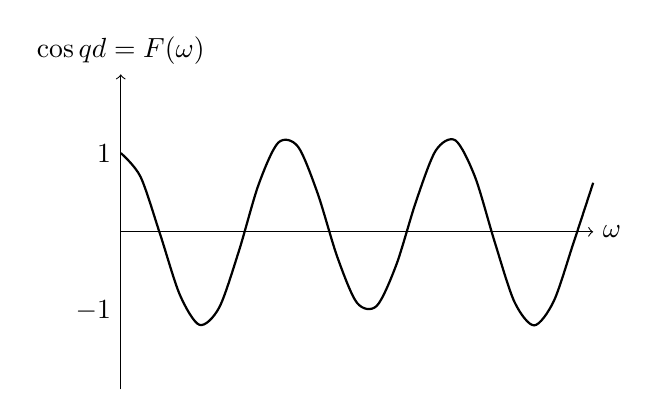
\begin{tikzpicture}
    \draw [->] (0, 0) -- (6, 0) node [right] {$\omega$};
    \draw [->] (0, -2) -- (0, 2) node [above] {$\cos qd=F(\omega)$};

    \draw [thick, domain=0.001:6] plot [smooth] (\x, {cos(deg(\x))*cos(2*deg(\x))-0.5*(2+0.5)*sin(deg(\x))*sin(2*deg(\x))});

    \draw (0,1) node [left] {$1$};
    \draw (0,-1) node [left] {$-1$};
  \end{tikzpicture}
\end{center}
By plotting $\omega$ against $q$, one can obtain a photonic band structure, with the gaps at $q=n\pi/d$. Here, the EM wave is attenuated and does not propagate along $\mathbf{\hat{z}}$. The bandgap occurs since there is no absorption since $\varepsilon_a,\varepsilon_b\in\mathbb{R}$, i.e. the wave is evanescent. 
\end{eg}
\begin{eg}[Photonic nanocavity]
Photonic crystals are easier to fabricate in two dimensions, simply by etching holes into a slab of high $k$ material surrounded by low $k$ material. In such 2D photonic crystals it is also possible to incorporate a defect in which a localised photonic mode can exist that emits within the bandgap of the 2D photonic crystal. This defines a photonic nanocavity.\\[5pt]
One application of such photonic nanocavities is in the field of cavity quantum electrodynamics. It is possible to position a small semiconductor quantum dot (QD), an "artificial atom", within the nanocavity. The emission spectrum is strongly modified if the nanocavity mode is designed to be close to the emission wavelength of the quantum dot (strong-coupling regime).\\[5pt]
The cavity mode can be tuned continuously, for example by adsorption of a self-assembled molecular layer on the surface. The strong interaction between the QD and the cavity mode results in the formation of so-called polariton modes. The lower (upper) polariton branch is cavity (QD)-like for positive detuning and QD(cavity)-like for negative detuning. For zero detuning the strong interaction prevents the crossing of the two dispersion relationships. This allows, for example, to control the exciton lifetime in the nanocavity. 
\end{eg}
\newpage
\subsection{Coherence}
For simplicity, in this discussion the waves will be taken to have scalar
amplitudes. Interference phenomena, diffraction etc, rely on the well defined phase between wavelets (determined by optical path lengths etc.) which are eventually summed for the overall wave amplitude. This can be exact only for purely monochromatic waves - a single, well-defined frequency. However, Fourier Theory means that only infinitely long (in time and space) waves can be purely monochromatic. Real sources and waves (even lasers) are at best `quasi-monochromatic'.
\begin{defi}[Coherence length, width]
Phase registration is lost over a distance $c\tau_c$, where $\tau_c$ is the (temporal) coherence length along the direction of propagation, and over a distance $x_c$, where $x_c$ is the (spatial) coherence width perpendicular to the direction of propagation.
\end{defi}
\begin{defi}[Temporal harmonics and power spectrum]
A time-dependent function $f(t)$ can be described in terms of its temporal harmonics $F(\omega)e^{i\omega t}$.
$$f(t)=\frac{1}{2\pi}\int_{-\infty}^\infty F(\omega)e^{i\omega t}d\omega,\quad F(\omega)=\int_{-\infty}^\infty f(t)e^{-i\omega t}d\omega$$
The power in the frequency range $[\omega,\omega+d\omega]$ is the power spectrum, i.e.
$$P(\omega)d\omega\sim|F(\omega)|^2d\omega$$
\end{defi}
\begin{eg}[Lasers]
For a pure harmonic wave of frequency $\omega_0$, say $f(t)\sim\cos(\omega_0t+\alpha)$:
$$F(\omega)=\frac{1}{2}\int\bigg(e^{i(\omega_0t+\alpha)}+e^{-i(\omega_0t+\alpha)}\bigg)e^{-i\omega t}dt\propto e^{i\alpha}\delta(\omega-\omega_0)+e^{-i\alpha}\delta(\omega+\omega_0)$$
i.e. a pair of delta functions at $\pm\omega_0$.
\end{eg}
\begin{eg}[Spectral lines]\leavevmode
\begin{enumerate}
    \item Lifetime broadening: Unstimulated emission from an isolated, stationary atom can be represented semi-classically as a decaying harmonic wave, beginning at $t = 0$ and characterized by a decay time $\tau_s$ or a scattering frequency $\omega_s = 1/\tau_s$:
    $$F(\omega)=\int_0^\infty e^{i\omega_0t}e^{-\omega_st}e^{-i\omega t}dt=\frac{1}{\omega-\omega_0-i\omega_s}\implies P(\omega)=\frac{1}{(\omega-\omega_0)^2+\omega_s^2}$$
    i.e. $P(\omega)$ is a Lorentzian peak centred on $\omega_0$ and with a linewidth (Full Width Half Maximum) of $2\omega_s$, determined by the decay time $\tau_s$.
    \item Thermal broadening: radiation from atoms moving along the line of sight (w.l.o.g. say $x$-axis) with velocity $v_x$ will be Doppler-shifted in frequency $\omega-\omega_0=\frac{\omega_0v_x}{c}$. The observed frequency spectrum will be a Gaussian since the distribution of atomic/molecular velocities is Gaussian.
    $$P(\omega)=Ce^{-(\omega-\omega_0)^2/2\sigma^2},\quad\sigma^2=\frac{\omega_0^2k_BT}{mc^2}$$
    the full-width half maximum in $\omega$-space will be
    $$2.36\omega_0\sqrt{\frac{k_BT}{mc^2}}=2.36\sigma$$
    \item Pressure broadening: In a gas, an individual atom is subject to collisions with other atoms, which at the very least perturb the phase correlation of the emitted wave before and after each collision. The mean time $\tau_1$ between collisions is:
    $$\tau_1=\frac{1}{4N\overline{v}A}\propto\sqrt{T}/p$$
    where $N$ is the number density of atoms of collision cross-section $A$ and with mean velocity $\overline{v}$, and $p$ is the pressure. This also produces another Lorentzian profile (irrespective of the natural lifetime $\tau$)
    $$P(\omega)\sim\frac{1}{(\omega-\omega_0)^2+1/\tau_1^2}$$
\end{enumerate}
For a gas discharge lamp, the output is the superposition of large numbers of independent photons from individual similar atoms. This is essentially harmonic with frequency $\omega_0$ say, but with an amplitude and phase which have some random fluctuations - quasi-monochromatic light. $\omega_0$ is the underlying harmonic wave, and the linewidth $\Delta\omega$ can be related to some overall broadening equivalent to a lifetime $\tau_s$.
\end{eg}
\begin{eg}[White light]
At the extreme, a large number of atoms of different emission frequencies, or oscillators in the surface of an incandescent black body, result in white light with a very broad power spectrum covering the visible. There is thus zero coherence.
\end{eg}
For a strongly correlated (strongly coherent) waveform, interference effects are very clear. But what about diffraction and interference using a quasi-monochromatic light? It turns out that interference ideas provide a useful quantified description for the degree of correlation, or degree of coherence, of the partially coherent wavefield arising from a light source.
\begin{defi}[Coherence]
Two wave sources are perfectly coherent if their frequency and waveform are identical and their phase difference is constant. This allows us to predict the amplitude and phase of the wavefield at some location $\mathbf{r_2}$ and time $t_2$ from the knowledge of that at location $\mathbf{r_1}$ and time $t_1$.
\end{defi}
\begin{Note}[Optical Stethoscope]
The optical stethoscope is an imaginary device for investigating the time and spatial variation of wavefields and their temporal (on two different wavefronts along the direction of propagation) and spatial coherence (on the same wavefront transverse to the direction of propagation). Two identical optical fibres sample the wavefield at points A$_1$ and A$_2$ and transfer the amplitudes of the wavefield to the closely spaced points B$_1$ and B$_2$ which act as point sources to generate an interference pattern on a screen P. The fibres are lossless and introduce identical phase shifts which can be ignored.
\end{Note}
\begin{defi}[Time average]
The time average for any function $g(t)$ is defined as
$$\langle g(t)\rangle=\lim_{T\rightarrow\infty}\frac{1}{T}\int_0^Tg(t)dt$$
\end{defi}
\begin{defi}[Mutual coherence function]
Suppose we can sample the wavefield $f$ at two different points at different times, i.e. $f_1$ at $\mathbf{r_1}$ at $t$ and $f_2$ at $\mathbf{r_2}$ at $t-\tau$, then the complex mutual coherence function $\Gamma$ is defined as
$$\Gamma(\mathbf{r_1},\mathbf{r_2},\tau)=\langle f_1(\mathbf{r_1},t)f_2^*(\mathbf{r_2},t-\tau)\rangle$$
\end{defi}
\begin{defi}[Degree of mutual coherence]
Normalize the mutual coherence function to yield the degree of mutual coherence
$$\gamma(\mathbf{r_1},\mathbf{r_2},\tau)=\frac{\Gamma(\mathbf{r_1},\mathbf{r_2},\tau)}{\sqrt{I_1I_2}},\quad I_1=\Gamma(\mathbf{r_1},\mathbf{r_1},0),~I_2=\Gamma(\mathbf{r_2},\mathbf{r_2},0)$$
where $I_1$ and $I_2$ are the mean intensities at $\mathbf{r_1}$ and $\mathbf{r_2}$. $\gamma(\mathbf{r_1}, \mathbf{r_2}, \tau)$ determines how effectively the disturbances (wavelets) originating from $\mathbf{r_1}$ and $\mathbf{r_2}$ can interfere. If $I_1$ and $I_2$ are equal and $|\gamma|\sim1$, then $I$ can vary down to zero, giving good fringe contrast, as will become clear.
\end{defi}
\begin{eg}
To investigate 
\begin{itemize}
    \item temporal coherence: compares the wavefield $A_1=f(t)$ at one time with the wavefield $A_2=f(t-\tau)$ at some earlier time, at the `same point' on the wavefront: $\tau\neq 0$, $\mathbf{r_1}=\mathbf{r_2}$. This configuration is an example of amplitude division, i.e. it principally examines the time dependence of the field.
    \item spatial coherence: compares the wavefield $A_1$ at one point $\mathbf{r_1}$ in space with the wavefield $A_2$ at some other point $\mathbf{r_2}$ at the same time and same wavefront: $\tau=0$, $\mathbf{r_1}\neq\mathbf{r_2}$. This configuration is an example of wavefront division, i.e. it principally examines the space dependence of the field.
\end{itemize}
\end{eg}
\newpage
\subsubsection{Temporal coherence}
\begin{defi}[Temporal coherence function]
Define the temporal coherence function for the wavefield to be
$$\Gamma(\tau)=\langle f(t)f^*(t-\tau)\rangle$$
\end{defi}
\begin{Note}
The time delay between the two rays $\tau=2d/c$ can be altered spatially by moving the retro-reflector. The output intensity depends on the spatially introduced time interval $\tau$:
$$I(\tau)=\langle[f(t)+f(t-\tau)][f^*(t)+f^*(t-\tau)]\rangle=2I_0+\langle f(t)f^*(t-\tau)\rangle+\langle f(t-\tau)f^*(t)\rangle=2I_0+2\text{Re}[\Gamma(\tau)]$$
since $\Gamma\in\mathbb{C}$, we have $\Gamma=|\Gamma(\tau)|e^{i\Delta(\tau)}$, then
$$I(\tau)=2I_0+2\text{Re}[\Gamma(\tau)]=2I_0+2|\Gamma(\tau)|\cos(\Delta(\tau))$$
$\Gamma(\tau)$ has an amplitude and a phase term which both depend on the path difference which determines $\tau$.
\end{Note}
\begin{defi}[Fringe visibility]
$$V=\frac{I_{\text{max}}-I_{\text{min}}}{I_{\text{max}}+I_{\text{min}}}$$
\end{defi}
\begin{eg}
If the waveform is quasi-monochromatic, $f(t)\sim e^{-i\omega_0t}=e^{-ik_0ct}$, then
$$\Gamma(\tau)=\langle f(t)f^*(t-\tau)\rangle\sim\frac{1}{T}\int_0^Te^{-i\omega_0t}e^{i\omega_0(t-\tau)}dt\sim e^{-i\omega_0\tau}=e^{-i2k_0d}$$
The phase term oscillates with changes in $d$ on the order of the wavelength of the light - rapidly compared with the variation in the amplitude $|\Gamma(\tau)|$. So if $I(\tau)$ is measured as $\tau=2d/c$ is varied, `fringes' are observed.
\end{eg}
\begin{cor}
$$V(\tau)=|\gamma(\tau)|$$
\end{cor}
\begin{proof}
We have $I_{\text{max}}=2I_0+2|\Gamma(\tau)|$ and $I_{\text{min}}=2I_0-2|\Gamma(\tau)|$, so $V(\tau)=\frac{|\Gamma(\tau|}{I_0}=|\gamma(\tau)|$, where $\gamma(\tau)$ is the normalized temporal coherence function.
\end{proof}
\begin{defi}[Autocorrelation]
The autocorrelation $h(\tau)$ of an irregular normalized waveform $f(t)$ is
$$h(\tau)=\int_{-\infty}^\infty f(t)f^*(t-\tau)dt$$
\end{defi}
\begin{remarks}
$h(\tau)$ is a measure of how $f$ at some time $t$ is correlated with $f$ at some other time. $h(\tau)$ must peak for $\tau=0$.
\end{remarks}
\begin{thm}[Wiener-Khinchine theorem]
$$H(\omega)=|F(\omega)|^2$$
where $H$ and $F$ are Fourier transforms of $h$ and $f$ respectively.
\end{thm}
\begin{proof}
$$H(\omega)=\int\int e^{-i\omega\tau}f(t)f^*(t-\tau)dtd\tau=\int\int e^{-i\omega(\tau+t)}f(t+\tau)e^{i\omega t}f^*(t)dtd\tau=F(\omega)F^*(\omega)$$
\end{proof}
\begin{remarks}
$h(\tau)$ and $\gamma(\tau)$ are similar, and only differ from a normalization factor. The Wiener-Khinchine theorem shows that the fringe visibility $V(\tau)$ for $f(t)$ is directly related to its power spectrum $P(\omega)$. For broadband light sources, no fringes are observable.
\end{remarks}
\begin{cor}
For real $f(t)$, the power spectrum of a light beam can be obtained by Fourier transforming the relative intensity $I_r(\tau)$ observed by introducing a time delay $\tau$ between two beams obtained by amplitude division.
\end{cor}
\begin{proof}
We have 
$$I(\tau)=2I_0+2\text{Re}[\Gamma(\tau)]\implies I_r(\tau)=1+\text{Re}[\gamma(\tau)]$$
since $f(t)\in\mathbb{R}$, we have $\gamma(\tau)=I_r(\tau)-1$. Since the power spectrum $P(\omega)$ is related ot the Fourier transform of $\gamma(\tau)$, it is in turn the Fourier transform of $I_r(\tau)-1$.
\end{proof}
\begin{Note}[Fourier transform spectroscopy]
The optical path of one beam can be varied with respect to the other introducing a measurable time delay $\tau=2d/c$. The compensator plate, identical to that forming the beamsplitter, ensures that the both optical paths are equivalent when the movable mirror is the same distance $d_0$ from the beamsplitter as is the fixed mirror. One beam is reflected internally at the beamsplitter, and one externally, which introduces a phase difference of $\pi$ which can be ignored.
\end{Note}
\begin{defi}[Coherence length and time]
We define the coherence length $\ell-c$ as the path difference $(2d)$ at which the visibility falls by a factor of $e$. $\ell_c$ is a measure of coherence time $\tau_c=\ell_c/c$.
\end{defi}
\begin{eg}[Broadened spectral line]
Suppose the power spectrum $P(\omega)$ has a Gaussian profile $P(\omega)\propto e^{-(\omega-\omega_0)^2/2\sigma^2}$. We obtain $\Gamma(\tau)$ from the Wiener-Khinchine theorem:
$$\Gamma(\tau)\sim \int e^{i\omega\tau}e^{-(\omega-\omega_0)^2/2\sigma^2}d\omega=e^{i\omega_0\tau}\int e^{iu\tau}e^{-u^2/2\sigma^2}du\sim e^{i\omega_0\tau}e^{-\sigma^2\tau^2/2}$$
where $u=\omega-\omega_0$. But $I(\tau)=2I_0+2|\Gamma(\tau)|\cos(\omega_0\tau)$, so
$$I_r=1+\exp(-\sigma^2\tau^2/2)\cos(\omega_0\tau)$$
so the visibility is $V(\tau)=e^{-\sigma^2\tau^2/2}$. The interferogram shows essentially the same fringes as for a truly monochromatic source, but the fringe visibility falls as $d$ increases. The spacing of the fringes ($I \sim\cos(2d\omega_0/c)$) gives the central frequency $\omega_0$ of the line. The visibility gradually decreases as the $d$ increases because the two beams are becoming less mutually coherent. The coherence length (directly measurable from the interferogram) is $\ell_c\approx c\sqrt{2}/\sigma$, where $\sigma$ determines the frequency linewidth $\delta\omega$ of the spectral line. $\delta\omega$ is usually the full width half maximum of the Gaussian profile $P(\omega)$.
$$2.36\sigma=\delta\omega\sim c\delta k=2\pi c\delta(1/\lambda)\sim 2\pi c\frac{\delta\lambda}{\lambda^2}$$
And hence the coherence length is
$$\ell_c\approx\frac{c\sqrt{2}}{\sigma}\sim\frac{2.36}{\pi\sqrt{2}}\frac{\lambda^2}{\delta\lambda}$$
For Kr$^{84}$ line, $\lambda=560$ nm with $\delta\lambda\sim 0.0002$ nm and so $\ell_c\sim 0.78$ m.
\end{eg}
\begin{remarks}
Fourier transform spectroscopy is particularly powerful in the infrared spectral range. FTIR (Fourier transform infrared spectroscopy) has two important advantages over conventional infrared spectrometers that use monochromators / diffraction gratings:
\begin{itemize}
    \item The radiation throughput is higher because it is not limited by the input slit width; the size of the detector in an FTIR can be as large as the central interference ring (Jacquinot advantage).
\item The signal-to-noise ratio is higher because as the mirror separation is scanned the signal is continuously falling on the detector. In contrast, in a grating spectrometer, only background signal is falling on the detector while the monochromator switches between wavelengths (Fellgett advantage).
\end{itemize}
The spectral resolution of a Fourier transform spectrometer is given by $\frac{\lambda}{\delta\lambda}=2\times m$, where $m$ is the number of fringes recorded (limited by the size of the spectrometer).
\end{remarks}
\begin{Note}[Spatial observation of temporal coherence]
A broadened spectral line source with coherence length $\ell_c=c\tau_c$ affects the fringes obtained with Young's slits. Waves at P from slits illuminated with a parallel beam have path lengths which differ by $\ell$. They become decreasingly mutually coherent as $\ell\rightarrow\ell-c$ and beyond, so the fringe visibility will decrease as P moves off-axis.
\end{Note}
\newpage
\subsubsection{Spatial coherence}
\begin{Note}[Extended source for double slit]
Young's slits illuminated not by a parallel beam but a beam of
wavelength $\lambda$ and finite angular width from an extended source with intensity variation $I(x)$ in its own plane. Each point on the source produces a set of $\cos^2$ fringes angularly offset from each other because of the different angles the points on the source make at O. So the fringe contrast on the screen is degraded. If the angular width of the source measured from O is $\alpha$, then the fringes from the two edges will be offset by $\alpha D$. The spacing of each set of fringes is $\lambda D/d$, so serious contrast degradation sets in if:
$$d>\frac{\lambda}{\alpha}\approx w_c$$
where $w_c$ is the coherence width. For the two rays shown:
$$r_{1,2}+\rho_{1,2}=\rho+R\pm\frac{d}{2}\sin\theta\pm\frac{d}[2]\sin\chi$$
Now take $\sin\theta\approx x/L$ and $\sin\chi\approx y/D$, so the phase difference for the rays arriving at P from the point $x$ is 
$$k(r_1+\rho_1-r_2-\rho_2)=kd(\sin\theta+\sin\chi)=kd\bigg(\frac{x}{L}+\frac{y}{D}\bigg)=2ks$$
The amplitude $\psi(y)$ at P arising from the source region $x\rightarrow x+dx$ is then
$$\psi(y)\sim e^{ik(\rho+R)}\sqrt{I(x)}(e^{iks}+e^{-iks})=e^{ik(\rho+R)}\sqrt{I(x)}2\cos kx$$
where $I(x)$ is the intensity profile of the source. If the extended source is incoherent (radiation from each point on it is uncorrelated with that from any other point), the net intensity at P is obtained by summing $\sum|\psi(y)|^2$:
$$I_y(d)=\int|\psi(y)|^2dx=2\int I(x)(1+\cos2 ks)dx=2I_0+2\text{Re}\bigg[e^{-ikdy/D}\int I(x)e^{-ikdx/L}dx\bigg]$$
Change variables $x\approx L\theta$, $y\approx D\chi$, so $I(x)dx\rightarrow I(\theta)d\theta$ and write $kd=u$, then the intensity on the screen as a function of $y$ and of the slit separation $d$ is
$$I_y(u)=2I_0+2I_0\text{Re}[e^{iu\chi}\gamma(u)],\quad\gamma)u)=\frac{1}{I_0}\int I(\theta)e^{-iu\theta}d\theta$$
Write $\gamma(u)=|\gamma(u)|e^{-i\beta}$, then since $u\chi=kyd/D$, then
$$\gamma_y(u)=2I_0+2I_0|\gamma(u)|\cos\bigg(\beta+\frac{kyd}{D}\bigg)$$
The offset $\beta$ is determined by the source angular profile $I(\theta)$.
\end{Note}
\begin{figure}[H]
    \centering
    \includegraphics[width=\linewidth]{spatialcoherence.JPG}
\end{figure}
This motivates the following theorem:
\begin{thm}[van Cittert-Zernike theorem]
The degree of lateral coherence is the Fourier transform of the angular intensity distribution of the source $I(\theta)$.
$$\gamma(u)=\frac{1}{I_0}\int I(\theta)e^{-iu\theta} d\theta=\frac{\mathcal{F}[I(\theta)]}{I_0}$$
\end{thm}
\begin{eg}
When $I(x)$ is symmetric about the axis of the system, $\gamma(u)\in\mathbb{R}$ and $\beta=0$ if $\gamma(u)>0$, $\beta=\pi$ if $\gamma(u)<0$. The visibility of the fringes is then $V=\gamma(u)$ when $u=kd$.
\end{eg}
\begin{eg}
Suppose the slits are illuminated by a distant, uniform line source (parallel to the slits) of angular width $\alpha$, i.e. $I(\theta)=J$ if $-\alpha/2\leq\theta\leq\alpha/2$, then
$$\gamma(u)=\frac{1}{I_0}\int_{-\alpha/2}^{\alpha/2}Je^{-iu\theta} d\theta=\sinc\frac{u\alpha}{2}$$
where $I_0=\alpha J$. The observed fringe contrast depends on $u\alpha/2$ and falls to zero at $u\alpha/2=\pi\alpha d/\lambda=\pi$ at $d=\lambda/\alpha$, beyond which $V$ becomes negative.
\end{eg}
\begin{eg}
A disc source of angular diameter $\alpha$ illuminating two pinholes separated by $d$, gives
$$\gamma(u)=\frac{2J_1(u\alpha/2)}{u\alpha/2}$$
For this circular symmetry, the fringe visibility falls to zero for $u\alpha/2=3.83$, and the coherence width is then $w_c=1.22\lambda/\alpha$.
\end{eg}
\begin{remarks}
The broader the source, the narrower the coherence width.
\end{remarks}
\begin{Note}
How does the fringes obtained for two pinhole apertures (hence the envelope profile) depend on their separation $d$ for fixed source width. As $d$ is increased, the fringe spacing falls, as does the fringe contrast, as the two pinholes becomes less mutually coherent. Due to the `sinc' form of the $\gamma(u)$ function, $V$ in fact goes through zero and then rises slightly.
\end{Note}
\begin{remarks}
In 2D, one can define a coherence area. Further account for temporal coherence gives us the coherence volume.
\end{remarks}
\begin{eg}
For sunlight ($\lambda\sim 500$ nm, $\delta\lambda\sim 500$ nm, $\alpha\sim 0.5\degree$), we have the coherence width and coherence length to be
$$w_c\sim\frac{\lambda}{\alpha}\sim 5\times10^{-5}m,\quad\ell_c\sim\frac{\lambda^2}{\delta\lambda}\sim 500 nm$$
For distant stars, $\alpha<<0.01$ radians, so their coherence widths at the Earth are much greater and can be exploited to measure their angular diameters.
\end{eg}
\begin{Note}[Michelson's stellar interferometer]
Since $\alpha$ is very small for stars, $w_c$ is several metres for visible wavelengths. Using a Young's slit set-up to observe the reduction in fringe contrast as $d$ is increased is impossible, as fringes with very small spacing would result. We may achieve variable large spacing $D$ using moveable mirrors to focus light to the fixed slits. The fringe visibility as a function of $D$ allows coherence widths on the scale of metres to be measured.
\end{Note}
\begin{eg}
Michelson used this to look at the star Betelgeuse. For $\lambda = 570$ nm, the fringes vanished at $D = 3.07$ m, corresponding then to $\alpha=22.6\times10^{-8}$ rad (0.047 sec of arc). Using the distance from the Earth determined independently by parallax measurements, this can be used to determine the diameter of the star, which is 950-1200 times the radius of the Sun.\\[5pt]
To create an image of the star one needs to know not the magnitude of the coherence function $|\gamma|$ but also its phase $\beta$. The difficulty in determining $\beta$ is that it is affected also by atmospheric jitter that can cause shifts of the interference pattern with respect to the optical axis of the telescope. To overcome this more than two entrance apertures, at least three apertures A$_1$, A$_2$ and A$_3$ can be used. If the apertures are selected such that the pairs A$_1$A$_2$, A$_2$A$_3$ and A$_1$A$_3$ produce interference fringes with different periods that can be measured simultaneously, the atmospheric phase shifts can be eliminated and the real phase of $\gamma$ can be determined (method of phase closure). This allows reconstructing an image of the star through Fourier transformation.
\end{eg}
\newpage
\section{Electrodynamics}
\subsection{Vector Potential from classical EM}
Mostly revision from IB Physics B.
\begin{thm}[Existence of Magnetic Vector Potential]
For a magnetic field $\mathbf{B}$ in $\mathbb{R}^3$, $\exists$ a corresponding magnetic vector potential $\mathbf{A}$ such that $\mathbf{B}=\boldsymbol{\nabla}\times\mathbf{A}$.
\end{thm}
\begin{proof}
Since $\boldsymbol{\nabla}\cdot\mathbf{B}=0$ and the divergence of a curl must be zero, $\exists\mathbf{A}$ such that $\mathbf{B}=\boldsymbol{\nabla}\times\mathbf{A}$. Note that $\mathbf{A}$ in $\mathbb{R}^n$ will only exist in a simply connected domain.
\end{proof}
\begin{thm}[Uniqueness of Magnetic Vector Potential]
$\mathbf{A}$ uniquely determines $\mathbf{B}$ but $\mathbf{B}$ does not uniquely determine $\mathbf{A}$.
\end{thm}
\begin{proof}
For the first part, suppose $\exists\mathbf{A_1},\mathbf{A_2}$ such that $\boldsymbol{\nabla}\times\mathbf{A_1}=\mathbf{B}$ and $\boldsymbol{\nabla}\times\mathbf{A_2}=\mathbf{B}$, then
$$\boldsymbol{\nabla}\times(\mathbf{A_2}-\mathbf{A_1})=\mathbf{B}-\mathbf{B}=0\implies\mathbf{A_1}=\mathbf{A_2}$$
But for the second part, consider evaluating
$$\boldsymbol{\nabla}\times(\mathbf{A}+\boldsymbol{\nabla}f)=\boldsymbol{\nabla}\times\mathbf{A}$$
where $f$ is some scalar function and hence $\boldsymbol{\nabla}\times(\boldsymbol{\nabla}f)=\boldsymbol{0}$ (curl of a gradient is zero). Hence, $\mathbf{B}$ is invariant under such gauge transformations. This is called gauge freedom.
\end{proof}
\begin{thm}[Poisson Equation for Magnetic Vector Potential]
In the magnetostatic case, the magnetic vector potential $\mathbf{A}$ satisfies the Poisson Equation $\nabla^2\mathbf{A}=-\mu_0\mathbf{J}$ with solutions
$$\mathbf{A}(\mathbf{r})=\frac{\mu_0}{4\pi}\int_{\mathcal{V}}\frac{\mathbf{J}(\mathbf{r'})}{|\mathbf{r}-\mathbf{r'}|}d^3r'$$
where $\mathcal{V}$ is a finite volume such that $\mathbf{A}=0$ at infinity. This is true if $\boldsymbol{\nabla}\cdot\mathbf{A}=0$ (Coulomb gauge).
\end{thm}
\begin{proof}
Assuming the Coulomb gauge holds, i.e. $\boldsymbol{\nabla}\cdot\mathbf{A}=0$: 
$$\mu_0\mathbf{J}=\boldsymbol{\nabla}\times\mathbf{B}=\boldsymbol{\nabla}\times(\boldsymbol{\nabla}\times\mathbf{A})=-\nabla^2\mathbf{A}+\boldsymbol{\nabla}(\boldsymbol{\nabla}\cdot\mathbf{A})=-\nabla^2\mathbf{A}$$
The corresponding solution will be $\mathbf{A}(\mathbf{r})=\int_V(-\mu_0\mathbf{J})G(\mathbf{r},\mathbf{r'})dV'$ where $G(\mathbf{r},\mathbf{r'})$ is the solution to $\nabla^2G(\mathbf{r},\mathbf{r'})=\delta(\mathbf{r'}-\mathbf{r})\implies G(\mathbf{r},\mathbf{r'})=-\frac{1}{4\pi|\mathbf{r}-\mathbf{r'}|}$, hence giving our result.
\end{proof}
\begin{cor}[Coulomb Gauge]
The Coulomb gauge is always true in magnetostatics.
\end{cor}
\begin{proof}
Here we will show the Coulomb gauge will always hold in magnetostatics. Suppose $\mathbf{A}$ is divergenceless but our original potential $\mathbf{A_0}$ is not, then if we add $\boldsymbol{\nabla}f$ for some scalar function $f$, the new divergence is $\boldsymbol{\nabla}\cdot\mathbf{A}=\boldsymbol{\nabla}\cdot\mathbf{A_0}+\nabla^2f$. Then we have $\nabla^2f=-\boldsymbol{\nabla}\cdot\mathbf{A_0}$ which is mathematically identical to the Poisson's equation in electrostatics. The corresponding solution will be
$$f(\mathbf{r})=\frac{1}{4\pi}\int G(\mathbf{r},\mathbf{r'})(\boldsymbol{\nabla}\cdot\mathbf{A_0})d^3r'$$
If $\boldsymbol{\nabla}\cdot\mathbf{A_0}$ does not go to zero at infinity, we will have to use other means to discover the appropriate $f$. Essentially, it is always possible to find a $f$ that obeys the Coulomb gauge, hence completing the proof. To verify this, we compute $\nabla\cdot\mathbf{A}$. Invoking the solution to Poisson's equation,
\begin{eqnarray}
\boldsymbol{\nabla}_r\cdot\mathbf{A}(\mathbf{r})&=&\frac{\mu_0}{4\pi}\int_{\mathcal{V}}\mathbf{J}(\mathbf{r'})\cdot\boldsymbol{\nabla}_{\mathbf{r}}\bigg(\frac{1}{|\mathbf{r}-\mathbf{r'}|}\bigg)d^3r'\nonumber\\&=&-\frac{\mu_0}{4\pi}\int_{\mathcal{V}}\mathbf{J}(\mathbf{r'})\cdot\boldsymbol{\nabla}_{\mathbf{r'}}\bigg(\frac{1}{|\mathbf{r}-\mathbf{r'}|}\bigg)d^3r'\nonumber\\&=&\frac{\mu_0}{4\pi}\bigg[\int_{\mathcal{V}}\boldsymbol{\nabla}_{\mathbf{r'}}\cdot\bigg(\frac{\mathbf{J}(\mathbf{r'})}{|\mathbf{r}-\mathbf{r'}|}\bigg)d^3r'-\int_{\mathcal{V}}(\boldsymbol{\nabla}_{\mathbf{r'}}\cdot\mathbf{J}(\mathbf{r'}))\bigg(\frac{1}{|\mathbf{r}-\mathbf{r'}|}\bigg)d^3r'\bigg]\nonumber\\&=&\frac{\mu_0}{4\pi}\bigg[\int_{\partial\mathcal{V}}\frac{\mathbf{J}(\mathbf{r'})}{|\mathbf{r}-\mathbf{r'}|}d^2r'+\int_{\mathcal{V}}\frac{\partial\rho(\mathbf{r')}}{\partial t}\frac{1}{|\mathbf{r}-\mathbf{r'}|}d^3r'\bigg]\nonumber
\end{eqnarray}
The first term vanish since currents are localized such that $\mathbf{J}=0$ on the boundary while the second term is zero since after invoking the continuity equation $\boldsymbol{\nabla}\cdot\mathbf{J}=-\frac{\partial\rho}{\partial t}$ (discussed later). But,  $\boldsymbol{\nabla}\cdot\mathbf{J}=0$ for magnetostatics, where we assumed $\rho=0$.
\end{proof}
\begin{cor}[Boundary Condition]
$\mathbf{A_\parallel}$ is continuous.
\end{cor}
\begin{proof}
By Stokes' theorem, the circulation of $\mathbf{A}$ around the loop equals the flux of $\mathbf{B}$ through the loop. As the width of the loop becomes infinitesimally small, the flux approaches zero and we recover the boundary condition.
\end{proof}
\begin{cor}[Biot-Savart Law]
The magnetic field induced by a volume current density $\mathbf{J}$, or if the current is localized on a surface with surface current $\mathbf{K}$, or on a curve with line current $I$, then respectively we have
$$\mathbf{B}=\frac{\mu_0}{4\pi}\int\mathbf{J}(\mathbf{r'})\times\frac{\mathbf{r}-\mathbf{r'}}{|\mathbf{r}-\mathbf{r'}|^3}dV',\quad\mathbf{B}=\frac{\mu_0}{4\pi}\int\mathbf{K}(\mathbf{r'})\times\frac{\mathbf{r}-\mathbf{r'}}{|\mathbf{r}-\mathbf{r'}|^3}dS',\quad\mathbf{B}=\frac{\mu_0I}{4\pi}\oint_Cd\mathbf{r'}\times\frac{\mathbf{r}-\mathbf{r'}}{|\mathbf{r}-\mathbf{r'}|^3}$$
\end{cor}
\begin{proof}
Taking the curl of the solution of the Poisson's Equation for magnetostatics,
$$\mathbf{B}=\frac{\mu_0}{4\pi}\int\boldsymbol{\nabla}_r\times\bigg(\frac{\mathbf{J}(\mathbf{r'})}{|\mathbf{r}-\mathbf{r'}|}\bigg)d^3r'=\frac{\mu_0}{4\pi}\int\mathbf{J}(\mathbf{r'})\times\frac{\mathbf{r}-\mathbf{r'}}{|\mathbf{r}-\mathbf{r'}|^3}d^3r'$$
The other results are obtained by noting that $\mathbf{J}dV=\mathbf{K}dS=Id\mathbf{r}$.
\end{proof}
\begin{thm}[Equivalence of Biot-Savart and Ampere's Law]
In magnetostatics, Biot-Savart Law and Ampere's law are equivalent.
\end{thm}
\begin{proof}
We previously showed that Ampere's Law implies the Biot-Savart Law. Conversely, consider an arbitrary current loop such that current $I$ traverses a closed loop $\mathcal{C}_1$. We trace out an arbitrary closed Amperian loop $\mathcal{C}_2$ that encloses the current $I$. We want to show that $\oint_{\mathcal{C}_2}\mathbf{B}\cdot d\mathbf{l}_2=\mu_0I$ where $\mathbf{B}$ is the magnetic field due to the current loop. From Biot-Savart Law, this is
$$\mathbf{B}=\int d\mathbf{B}=\oint_{\mathcal{C}_1}\frac{\mu_0I}{4\pi}\frac{d\mathbf{l_1}\times\mathbf{\hat{r}}}{r^2}$$
Then, evaluating $\oint_{\mathcal{C}_2}\mathbf{B}\cdot d\mathbf{l_2}$,
$$\oint_{\mathcal{C}_2}\mathbf{B}\cdot d\mathbf{l_2}=\frac{\mu_0I}{4\pi}\oint_{\mathcal{C}_1}\oint_{\mathcal{C}_2}\frac{(d\mathbf{l_1}\times\mathbf{\hat{r}})\cdot d\mathbf{l_2}}{r^2}=\frac{\mu_0I}{4\pi}\oint_{\mathcal{C}_1}\oint_{\mathcal{C}_2}\frac{(d\mathbf{l}_2\times d\mathbf{l}_1)\cdot\mathbf{\hat{r}}}{r^2}$$
But $(d\mathbf{l_2}\times d\mathbf{l}_1)$ is an area element $d\mathbf{A}$, which is the infinitesimal area bounded by $\mathcal{C}_2$ and $\mathcal{C}_2$ displaced in the $d\mathbf{l_1}$ direction. Further, $-\frac{\mathbf{\hat{r}}\cdot d\mathbf{A}}{r^2}$ is the solid angle subtended by $d\mathbf{A}$ viewed from the point on the current loop $\mathcal{C}_1$. Adding all the solid angles as we traverse around the current loop, we will get the net change from an initial point to a final point, both on the current loop.\\[5pt]
If $\mathcal{C}_2$ encloses the current $I$, then this net change in solid angle is $4\pi$. This is true since the initial solid angle is $2\pi$, which upon traversing the current loop, it decreases, becomes zero at some point, and then $-2\pi$. Otherwise, if $\mathcal{C}_2$ does not enclose the current $I$, then the net change in solid angle is clearly zero. Hence, proving Ampere's Law.
\end{proof}
\begin{Note}[Procedure for Biot-Savart Law]
The general methodology for problems involving line currents will be:
\begin{enumerate}
    \item Identify the position vector of the source point.
    \item Identify the position vector of the field point.
    \item Find the unit relative position vector which points from the source point to the field point, $\mathbf{\hat{r}'}$.
    \item Evaluate  $d\mathbf{s}\times\mathbf{\hat{r}'}$, where $d\mathbf{s}$ is parallel to the current $I$.
    \item Evaluate Biot-Savart Law.
\end{enumerate}
\end{Note}
\begin{remarks}
The flux through any surface $S$ is equal to the line integral of $\mathbf{A}$ around the closed loop $L$. This follows from Stokes' theorem.
$$\Phi_S=\int_S\mathbf{B}\cdot d\mathbf{S}=\oint_{\partial S}\mathbf{A}\cdot d\mathbf{l}$$
Hence, the flux through any surface bounded by the closed path $L$ depends only on properties on the path $L$.
\end{remarks}
\begin{Note}
The vector potential $\mathbf{A}$ can be calculated by:
\begin{itemize}
    \item direct calculation from the current distribution via the Poisson equation
    \item integration of a known $\mathbf{B}$ field by definition
    \item equating the line integral of $\mathbf{A}$ to the flux through any surface bounded by the path of the line integral.
\end{itemize}
\end{Note}
\begin{prop}
The fields $\mathbf{E}$ and $\mathbf{B}$ can be written in terms of the potentials $\phi$ and $\mathbf{A}$. These potential have gauge freedom.
\end{prop}
\begin{proof}
From Faraday's Law and the definition of $\mathbf{A}$, we have
$$\boldsymbol{\nabla}\times\bigg(\mathbf{E}+\frac{\partial\mathbf{A}}{\partial t}\bigg)=0$$
We can set the expression $\mathbf{E}+\frac{\partial\mathbf{A}}{\partial t}$ to be $-\boldsymbol{\nabla}\phi$ such that it is still valid. For $\mathbf{B}$, we just have $\mathbf{B}=\boldsymbol{\nabla}\times\mathbf{A}$. Now suppose $\mathbf{A}$ becomes $\mathbf{A'}=\mathbf{A}+\boldsymbol{\nabla}f$, then in order for $\frac{\partial\mathbf{A'}}{\partial t}+\boldsymbol{\nabla}\phi'=\frac{\partial\mathbf{A}}{\partial t}+\boldsymbol{\nabla}\phi$, we must have
$$\phi'=\phi-\frac{\partial f}{\partial t}$$
when we have $\mathbf{A'}=\mathbf{A}+\boldsymbol{\nabla}f$.
\end{proof}
\begin{defi}[Lorenz Gauge]
The Lorenz gauge is $\boldsymbol{\nabla}\cdot\mathbf{A}=-\mu_0\varepsilon_0\frac{\partial\phi}{\partial t}$ which reduces to the Coulomb gauge when the fields are static.
\end{defi}
\begin{prop}
The inhomogeneous wave equations in terms of potentials will be
$$\nabla^2\mathbf{A}-\frac{1}{c^2}\frac{\partial^2\mathbf{A}}{\partial t^2}=-\mu_0\mathbf{J}$$
$$\nabla^2\phi-\frac{1}{c^2}\frac{\partial^2\phi}{\partial t^2}=-\frac{\rho}{\varepsilon_0}$$
\end{prop}
\begin{proof}
From Gauss' Law,
$$\frac{\rho}{\varepsilon_0}=\boldsymbol{\nabla}\cdot\mathbf{E}=-\frac{\partial}{\partial t}\boldsymbol{\nabla}\cdot\mathbf{A}-\nabla^2\phi$$
From Ampere's Law,
$$\boldsymbol{\nabla}\times(\boldsymbol{\nabla}\times\mathbf{A})=\mu_0\mathbf{J}-\mu_0\varepsilon_0\frac{\partial}{\partial t}\bigg(\frac{\partial\mathbf{A}}{\partial t}+\boldsymbol{\nabla}\phi\bigg)$$
The left hand side is simply $\boldsymbol{\nabla}(\boldsymbol{\nabla}\cdot\mathbf{A})-\nabla^2\mathbf{A}$ as before. So re-arranging
$$\boldsymbol{\nabla}\bigg(\boldsymbol{\nabla}\cdot\mathbf{A}+\mu_0\varepsilon_0\frac{\partial\phi}{\partial t}\bigg)=\nabla^2\mathbf{A}+\mu_0\mathbf{J}-\mu_0\varepsilon_0\frac{\partial^2\mathbf{A}}{\partial t^2}$$
Taking the left hand side to be zero, i.e. Lorenz gauge, we recover both desired inhomogeneous wave equations.
\end{proof}
\begin{defi}[d'Alembertian]
More common to write  $\nabla^2-\frac{1}{c^2}\frac{\partial^2}{\partial t^2}$ as the d'Alembertian $\Box$.
$$\Box:=\nabla^2-\frac{1}{c^2}\frac{\partial^2}{\partial t^2}$$
\end{defi}
\begin{thm}[Multipole Expansion for Current Density]
The multipole expansion of $\mathbf{A}$ for a current-carrying loop $\mathcal{C}$ (does not need to be planar), where $|\mathbf{r}|>>|\mathbf{r'}|$, is
$$\mathbf{A}=\frac{\mu_0I}{4\pi}\oint_{\mathcal{C}}\bigg(\frac{1}{|\mathbf{r}|}+\frac{\mathbf{r}\cdot\mathbf{r'}}{|\mathbf{r}|^3}+...\bigg)d\mathbf{r'}$$
such that the leading order term is the magnetic dipole term which is equal to $\frac{\mu_0}{4\pi}\frac{I\mathbf{S}\times\mathbf{r}}{|\mathbf{r}|^3}$. 
\end{thm}
\begin{proof}
Since $|\mathbf{r}|$ is a constant with respect to the integration variable $\mathbf{r'}$, the monopole term, involving the closed loop integral $\oint_{\mathcal{C}}d\mathbf{r'}$, will give zero. We evaluate the second term (dipole term). For a constant vector $\mathbf{C}$, and integrating about $\mathcal{C}=\partial S$, where $S$ is the surface bounded by the closed loop $\mathcal{C}$. Evaluating $\oint_{\mathcal{C}}(\mathbf{C}\cdot d\mathbf{r})\frac{\mathbf{r}\cdot\mathbf{r'}}{|\mathbf{r}|^3}$ gives
$$\oint_{\mathcal{C}}\bigg(C_w\frac{r_jr_j'}{|\mathbf{r}|^3}\bigg)dr_w'=\int_{\mathcal{S}}\varepsilon_{kli}\frac{\partial}{\partial r_k'}\bigg(\frac{C_lr_jr_j'}{|\mathbf{r}|^3}\bigg)dS_i'=\int_{\mathcal{S}}\varepsilon_{ikl}\delta_{k,j}\frac{C_lr_j}{|\mathbf{r}|^3}dS_i'=\frac{C_lr_j}{|\mathbf{r}|^3}\varepsilon_{ijl}S_i=C_i\frac{r_j}{|\mathbf{r}|^3}\varepsilon_{lji}S_l$$
where we used the Stokes' Theorem $\oint_{\partial\mathcal{S}}(\alpha C_w)dr_w=\int_{\mathcal{S}}\varepsilon_{ijk}\partial_i(\alpha C_j) dS_k$ and relabelled the dummy indices at the end. The right side is basically $\mathbf{C}\cdot(\mathbf{S}\times\frac{\mathbf{r}}{|\mathbf{r}|^3})$. Hence, $\oint_{\mathcal{C}}\frac{\mathbf{r}\cdot\mathbf{r'}}{|\mathbf{r}|^3}(\mathbf{C}\cdot d\mathbf{r})-\mathbf{C}\cdot(\mathbf{S}\times\frac{\mathbf{r}}{|\mathbf{r}|^3})=\mathbf{C}\cdot(\oint_{\mathcal{C}}\frac{\mathbf{r}\cdot\mathbf{r'}}{|\mathbf{r}|^3}d\mathbf{r}-\mathbf{S}\times\frac{\mathbf{r}}{|\mathbf{r}|^3})=0$ where $\mathbf{C}$ is a constant vector. Since $\mathbf{C}$ is arbitrary vector, the vector expression in the brackets is the null vector, and hence the dipole contribution is $\frac{\mu_0I}{4\pi}\oint_{\mathcal{C}}\frac{r_jr_j'}{|\mathbf{r}|^3}dr_i'=\frac{\mu_0I}{4\pi}\frac{\mathbf{S}\times\mathbf{r}}{|\mathbf{r}|^3}$. 
\end{proof}
\begin{cor}
In terms of the current density, the magnetic dipole moment is $\frac{1}{2}\int\mathbf{r'}\times\mathbf{J}(\mathbf{r'})d^3r'$. 
\end{cor}
\begin{proof}
We rewrite $\mathbf{A_{dipole}}$ as $\frac{\mu_0}{4\pi}\int\frac{(\mathbf{r}\cdot\mathbf{r'})}{|\mathbf{r}|^3}\mathbf{J}(\mathbf{r'})d^3r'$. Omitting the $\frac{\mu_0}{4\pi|\mathbf{r}|^3}$ factor, we have
$$\int r_jr_j'J_id^3r'=-\frac{1}{2}r_j\int(r_i'J_j-r_j'J_i)d^3r'=-\frac{1}{2}\varepsilon_{ijk}r_j\int(\mathbf{r'}\times\mathbf{J})_kd^3r'=-\frac{1}{2}\mathbf{r}\times\bigg[\int(\mathbf{r'}\times\mathbf{J}(\mathbf{r'}))d^3r'\bigg]_i$$
To have $\mathbf{A_{dipole}}=\frac{\mu_0}{4\pi}\frac{\mathbf{m}\times\mathbf{r}}{|\mathbf{r}|^3}$, we must have $\mathbf{m}=\frac{1}{2}\int\mathbf{r'}\times\mathbf{J}(\mathbf{r'})d^3r'$.
\end{proof}
\begin{remarks}
By considering an infinite solenoid, one realizes that the magnetic field outside is zero (from Ampere's law). But yet, from
$$\int_S\mathbf{B}\cdot d\mathbf{S}=\oint_{\partial S}\mathbf{A}\cdot d\mathbf{L}$$
then, we have respectively $A_\phi=\frac{\mu_0nIr}{2}$ and $A_\phi=\frac{\mu_0nIa^2}{2r}$ inside and outside. Despite $\mathbf{B}=0$ outside, $\mathbf{A}\neq\boldsymbol{0}$.
\end{remarks}
\newpage
\subsection{Vector Potential for quantum mechanics}
A particle of mass $m$ and charge $q$ can be described by the Lagrangian $\mathcal{L}=\frac{1}{2}m|\mathbf{\dot{x}}|^2+q\mathbf{\dot{x}}\cdot\mathbf{A}-q\phi$ with corresponding equation of motion $m\mathbf{\ddot{x}}=q(\mathbf{E}+\mathbf{\dot{x}}\times\mathbf{B})$. 
\begin{defi}[Canonical momentum]
$$\mathbf{p}=\frac{\partial\mathcal{L}}{\partial\mathbf{\dot{x}}}=m\mathbf{\dot{x}}+q\mathbf{A}$$
\end{defi}
The Hamiltonian is 
$$H=\mathbf{\dot{x}}\cdot\mathbf{p}-\mathcal{L}=\frac{1}{2m}(\mathbf{p}-q\mathbf{A})^2+q\phi$$
This is called minimal coupling (shift of kinetic energy to include $\mathbf{A}$). 
\begin{remarks}
In the quantum theory, we have the canonical commutation relations $[x_i,p_j]=\delta_{ij}$ and $[x_i,x_j]=0=[p_i,p_j]$. $p$ is the canonical momentum and not $m\mathbf{\dot{x}}$.
\end{remarks}
\begin{remarks}
The canonical momentum $\mathbf{p}$ is not gauge invariant since it transforms as $\mathbf{p}\rightarrow\mathbf{p}+q\boldsymbol{\nabla}\alpha$, and hence not physical. Only quantities that are gauge invariant should be viewed as physical. 
\end{remarks}
We promote the classical operators to quantum operators, i.e. $\mathbf{p}\rightarrow -i\hbar\boldsymbol{\nabla}$. Then the time-dependent Schr\"{o}dinger's equation is
$$i\hbar\frac{\partial}{\partial t}\psi=H\psi=\frac{1}{2m}(-i\hbar\boldsymbol{\nabla}-q\mathbf{A})^2\psi+q\phi\psi$$
We need to use the gauge fields $\mathbf{A}$ and $\phi$ to formulate the theory at the quantum level. Under a gauge transformation, the wavefunction should change as $\psi\mapsto e^{iq\alpha/\hbar}\psi$, so to ensure the physical probabilities $|\psi|^2$ invariant. With this choice, the Schr\"{o}dinger's equation is covariant. 
\begin{prop}
By defining the covariant derivatives as 
$$D_t\psi:=\frac{\partial\psi}{\partial t}+i\frac{q\phi}{\hbar}\psi,\quad D_i\psi:=\frac{\partial\psi}{\partial x^i}-i\frac{qA_i}{\hbar}\psi$$
then the Schr\"{o}dinger's equation has a covariant form
$$i\hbar D_t\psi=-\frac{\hbar^2}{2m}D_iD_i\psi$$
\end{prop}
\begin{proof}
Under a gauge transformation, $D_t\psi\mapsto e^{iq\alpha/\hbar}D_t\psi$ and $D_i\psi\mapsto e^{iq\alpha/\hbar}D_i\psi$. The Schr\"{o}dinger Equation becomes $i\hbar D_t\psi=-\frac{\hbar^2}{2m}D_iD_i\psi$ and this transforms covariantly.
\end{proof}
\subsubsection{Aharonov-Bohm Effect}
\begin{Note}[Particles moving around a flux tube]
A quantum particle can be offsetted by $\mathbf{A}\neq\boldsymbol{0}$, even in region where $\mathbf{B}=\boldsymbol{0}=\mathbf{E}$. Consider a particle moving on a circle around a solenoid of fixed radius $r$. Although $\mathbf{B}=\boldsymbol{0}$ on the circle, $\mathbf{A}\neq\boldsymbol{0}$ since
$$\oint\mathbf{A}\cdot d\mathbf{x}=\int\mathbf{B}\cdot d\mathbf{S}=\Phi_{total}=\Phi$$
We can take $A_\phi=\frac{\Phi}{2\pi r}$. The Hamiltonian is 
$$H=\frac{1}{2m}(p_\phi-qA_\phi)^2=\frac{1}{2mr^2}\bigg(-i\hbar\frac{\partial}{\partial\phi}-q\frac{\Phi}{2\pi}\bigg)^2$$
The energy eigenstates are $\psi=\frac{1}{\sqrt{2\pi r}}e^{in\phi}$, $n\in\mathbb{Z}$ with energy $E=\frac{1}{2mr^2}(n\hbar -q\frac{\Phi}{2\pi})^2=\frac{\hbar^2}{2mr^2}(n-\frac{\Phi}{\Phi_0})^2$ where $\Phi_0=\frac{2\pi\hbar}{q}$ is the quantum flux. The spectrum thus remains unchanged when $\Phi=m\Phi_0$, for $m\in\mathbb{Z}$. But it depends on $\Phi$ otherwise. Here, the energy of the particle knows about the flux $\Phi$ even though it never goes near the region with magnetic field.\\[5pt]
Another way of seeing this: Outside the solenoid, $\mathbf{B}=\boldsymbol{0}=\mathbf{E}$ and so $\mathbf{A}=\boldsymbol{\nabla}\alpha$ with $\alpha=\frac{\Phi}{2\pi}\phi$. We can remove $\mathbf{A}$ by redefining the wavefunction
$$\psi\rightarrow\tilde{\psi}=e^{-iq\alpha/\hbar}\psi=e^{-i\phi(\Phi/\Phi_0)}\psi$$
But $\tilde{\psi}$ should be single-valued and so $\Phi/\Phi_0\in\mathbb{Z}$. Otherwise, we cannot remove $\mathbf{A}$. The above gauge transformation is only allowed if $\Phi$ is an integer multiple of $\Phi_0$. This gives a first glimpse of topology in quantum mechanics.
\end{Note}
\begin{Note}[Aharonov-Bohm Scattering]
It was Aharonov and Bohm who first pointed out that a quantum particle can be affected by $\mathbf{A}$ even in regions void of $\mathbf{B}$. Consider a modification to the Young's double slit experiment where a solenoid is present. The particles do not enter the solenoid, yet the interference pattern depend on $\Phi/\Phi_0$. The particle obeys the Schr\"{o}dinger's equation
$$H\psi=\frac{1}{2m}(-i\hbar\boldsymbol{\nabla}-q\mathbf{A})^2\psi=E\psi$$
subject to some boundary conditions. We can formally remove $\mathbf{A}$ by writing 
$$\psi(\mathbf{x})=\exp\bigg(\frac{iq}{\hbar}\int^x\mathbf{A}(\mathbf{x'})\cdot d\mathbf{x'}\bigg)\chi(x)$$
where the integral is over any path. The phase picked up by the particle due to the gauge field differs depending on the path taken. How does the phase difference $\Delta\theta$ depend on the flux $\Phi$? Since $\chi(x)$ does not depend on $\mathbf{A}$, we can focus on the phase
$$\Delta\theta=\frac{q}{\hbar}\oint\mathbf{A}\cdot d\mathbf{x}=q\hbar\int\mathbf{B}\cdot d\mathbf{S}=q\frac{\Phi}{\hbar}$$
This is the Aharanov-Bohm phase. This manifests in the interference pattern seen on the screen. As $\Phi$ is changed, the interference pattern shifts, an effect which has been experimentally observed. Only when $\Phi$ is an integer multiple of $\Phi_0$ is the particle unaware of the presence of the solenoid.
\end{Note}
\begin{eg}[SQUID]
The Aharonov-Bohm effect also forms the basis for the operation of the `SQUID' (Superconducting QUantum Interference Device). A SQUID comprises a superconducting ring with two Josephson junctions. The two halves of the ring are connected to external leads. When a magnetic flux penetrates the ring a screening current is set up in the ring, which increases the current through one half of the ring and reduces it in the other half. This modulates the critical current of the Josephson junctions. It can be shown
that the current through the ring is 
$$I=I_c\sin(\Delta\theta)\sin\frac{\pi\Phi}{\Phi_0}$$
where $I_c$ is the critical current of the Josephson junctions in the absence of a magnetic flux and $\Phi_0$ is the flux quantum. Sensitivities of order $10^{−15}$ T are achievable, making SQUIDs useful for high sensitivity applications.
\end{eg}
\subsubsection{Superconductors}
\begin{defi}[Messiner effect]
Below some transition temperature $T_s$, superconductors exhibit zero resistance and expels all static magnetic fields.
\end{defi}
\begin{prop}[London equation]
Model the superconductor as a semiclassical system of surface current $\mathbf{J_s}$ with no damping to the motion of the charges.
$$\mathbf{J_s}=-\frac{1}{\mu_0\lambda_L^2}\mathbf{A}$$
where $\lambda_L=\sqrt{\frac{m}{n_s\mu_0q^2}}$ is the London penetration depth.
\end{prop}
\begin{proof}
We have
$$\frac{d}{dt}\mathbf{J_s}=\frac{d}{dt}(n_sq\mathbf{v})=n_sq\frac{q\mathbf{E}}{m}$$
Take the curl and use Faraday's equation, we then have $\boldsymbol{\nabla}\times\mathbf{J_s}+\frac{n_sq^2}{m}\mathbf{B}$ to be a constant. Since $\mathbf{B}=\boldsymbol{\nabla}\times\mathbf{A}$, the result follows.
\end{proof}
\begin{cor}
Under static conditions, magnetic fields decay exponentially in the superconductor.
\end{cor}
\begin{proof}
Under static conditions $\boldsymbol{\nabla}\times\mathbf{B}=\mu_0\mathbf{J_s}$, we then have
$$\boldsymbol{\nabla}\times(\boldsymbol{\nabla}\times\mathbf{B})=-\nabla^2\mathbf{B}=\mu_0\boldsymbol{\nabla}\times\mathbf{J_s}=-\frac{1}{\lambda_L^2}\boldsymbol{\nabla}\times\mathbf{A}$$
which gives us $B(x)=B(0)e^{-x/\lambda_L}$, i.e. exponentially decaying field. The superconducting current must lie near the surface.
\end{proof}
\begin{Note}[Fluxoid]
the carriers in a superconductors are in a Bose-condensed state with wavefunctions $\psi(l)=\sqrt{n_s}e^{i\theta(l)}$ where $l$ is the linear distance around the loop. The current density is
$$\mathbf{J_s}=q\psi^*(l)\mathbf{\hat{v}}\psi(l)=\frac{n_sq}{m}(\hbar\boldsymbol{\nabla}\theta(l)-q\mathbf{A})$$
Take a closed path $C$ through the interior of the loop, well away from its surface, so $\mathbf{B}=0$ and so $J_s=0$ by the London equation. The total phase change will round the contour $C$ will be
$$\oint_C\boldsymbol{\nabla}\theta(l)\cdot d\mathbf{l}=\frac{q}{\hbar}\oint_C\mathbf{A}\cdot d\mathbf{l}=\frac{q}{\hbar}\Phi_C$$
where $\Phi_C$ is the total magnetic flux through $C$. Since $\psi(l)$ must be single-valued, the total phase change round $C$ must be $2n\pi$, $n\in\mathbb{Z}$. Hence,
$$\Phi_c=\frac{\hbar}{q}2n\pi=n\frac{h}{q}=n\frac{h}[2e],\quad n\in\mathbb{Z}$$
The quanta $h/2e$ is called a fluxoid.
\end{Note}
\subsubsection{Magnetic Monopoles}
\begin{defi}[Magnetic monopoles]
A magnetic monopole is a hypothetical particle which emits a radial magnetic field
$$\mathbf{B}=\frac{g}{4\pi r^2}\mathbf{\hat{r}}\implies\int_{\mathcal{S}^2}\mathbf{B}\cdot d\mathbf{S}=g$$
where $g$ is the magnetic charge. They are forbidden by the Maxwell equation $\boldsymbol{\nabla}\cdot\mathbf{B}=0$, but most physicists expect that they exist. 
\end{defi}


\begin{Note}[Dirac quantization condition]
Consider a particle of charge $q$ localized in some region of space. If it travels on a closed path $\mathcal{C}$, it picks up a Aharonov-Bohm phase $\psi\rightarrow e^{iq\alpha/\hbar}\psi$ with $\alpha=\oint_{\mathcal{C}}\mathbf{A}\cdot \mathbf{x}=\oint_S\mathbf{B}\cdot d\mathbf{S}$. This phase is really a phase difference. Consider the particle moving in the background of a magnetic monopole. If it moves a path $\mathcal{C}$, it returns with a phase $\alpha=\int_S\mathbf{B}\cdot d\mathbf{S}=\frac{\Omega}{4\pi}g$ where $\Omega$ is the solid angle subtended by $S$. But there is an ambiguity. We could have also chosen to use $S'$ (see Figure 24) such that the phase is instead $\alpha'=-\frac{4\pi-\Omega}{4\pi}g$. But for consistency, we must have
$$e^{i\alpha q/\hbar}=e^{i\alpha'q/\hbar}\implies gq=2\pi\hbar m,\quad m\in\mathbb{Z}$$
Any magnetic charge must be related to any electric charge in this way.
\end{Note}
\newpage
\subsection{General solution for potentials}
\begin{prop}
Under Lorenz Gauge, the Maxwell's Equations become
$$-\nabla^2\phi+\frac{1}{c^2}\frac{\partial^2\phi}{\partial t^2}=\frac{\rho}{\varepsilon_0},\quad-\nabla^2\mathbf{A}+\frac{1}{c^2}\frac{\partial^2\mathbf{A}}{\partial t^2}=\mu_0\mathbf{J}$$
\end{prop}
\begin{proof}
In general, the electric field is written in terms of a scalar potential $\phi$ and a vector potential $\mathbf{A}$ such that
$$\mathbf{E}=-\boldsymbol{\nabla}\phi-\frac{\partial\mathbf{A}}{\partial t}\implies-\mu_0\varepsilon_0\frac{\partial\mathbf{E}}{\partial t}=\frac{1}{c^2}\boldsymbol{\nabla}\frac{\partial\phi}{\partial t}+\frac{1}{c^2}\frac{\partial^2\mathbf{A}}{\partial t^2}$$
Recall Ampere-Maxwell's Law and the identity $\boldsymbol{\nabla}\times\mathbf{B}=\boldsymbol{\nabla}\times(\boldsymbol{\nabla}\times\mathbf{A})=\boldsymbol{\nabla}(\boldsymbol{\nabla}\cdot\mathbf{A})-\nabla^2\mathbf{A}$, then we have
$$\mu_0\mathbf{J}=\boldsymbol{\nabla}\times\mathbf{B}-\mu_0\epsilon_0\frac{\partial\mathbf{E}}{\partial t}=-\nabla^2\mathbf{A}+\frac{1}{c^2}\frac{\partial^2\mathbf{A}}{\partial t^2}+\boldsymbol{\nabla}\bigg(\boldsymbol{\nabla}\cdot\mathbf{A}+\frac{1}{c^2}\frac{\partial\phi}{\partial t}\bigg)$$
Under Lorenz gauge, i.e. $\boldsymbol{\nabla}\cdot\mathbf{A}=-\frac{1}{c^2}\frac{\partial\phi}{\partial t}$, the equivalent form of Ampere-Maxwell's law is
$$-\nabla^2\mathbf{A}+\frac{1}{c^2}\frac{\partial^2\mathbf{A}}{\partial t^2}=\mu_0\mathbf{J}$$
To recover the other equation, we look at Gauss' Law again
$$\frac{\rho}{\varepsilon_0}=\boldsymbol{\nabla}\cdot\mathbf{E}=-\nabla^2\phi-\frac{\partial}{\partial t}(\boldsymbol{\nabla}\cdot\mathbf{A})=-\nabla^2\phi+\frac{1}{c^2}\frac{\partial^2\phi}{\partial t^2}$$
where we invoked the Lorenz gauge again.
\end{proof}
\begin{remarks}
These are wave equations with source terms given by the free charges and currents of the system. The general solutions take the form $f(t\pm r/c)$.
\end{remarks}
\begin{prop}
The general solution will then be
$$\phi(\mathbf{r},t)=\frac{1}{4\pi\epsilon_0}\int_{\mathbb{R}^3}\frac{\rho(\mathbf{r'},t-(|\mathbf{r}-\mathbf{r'}|/c))dV'}{|\mathbf{r}-\mathbf{r'}|},\quad \mathbf{A}(\mathbf{r},t)=\frac{1}{4\pi\epsilon_0}\int_{\mathbb{R}^3}\frac{\mathbf{J}(\mathbf{r'},t-(|\mathbf{r}-\mathbf{r'}|/c))dV'}{|\mathbf{r}-\mathbf{r'}|}$$
These are the retarded potentials which allows for the propagation of information at a finite speed $c$. The potential at $\mathbf{r}$ at time $t$ depends on the source at $\mathbf{r'}$ at a time $|\mathbf{r}-\mathbf{r'}|/c$ earlier.
\end{prop}
\begin{proof}
We solve this by performing Fourier Transform with time:
$$A^\mu(t,\mathbf{x})=\frac{1}{\sqrt{2\pi}}\int_{-\infty}^\infty\tilde{A}^\mu(\omega,\mathbf{x})e^{i\omega t}d\omega,\quad J^\mu(t,\mathbf{x})=\frac{1}{\sqrt{2\pi}}\int_{-\infty}^\infty\tilde{J}^\mu(\omega,\mathbf{x})e^{i\omega t}d\omega$$
such that $\Box A^\mu=-\mu_0J^\mu$ gives $(\nabla^2+k^2)\tilde{A}^\mu=-\mu_0\tilde{J}^\mu$ in Fourier space, where $k=\omega/c$. We solve this resultant equation (sourced Helmholtz equation) by finding the Green's function (see IB Methods) for $\nabla^2+k^2$, i.e. the $G(x,x')$ that satisfies
$$(\nabla^2+k^2)G(\mathbf{x},\mathbf{x'})=\delta^{(3)}(\mathbf{x}-\mathbf{x'})\implies\tilde{A}^\mu(\omega,\mathbf{x})=-\mu_0\int\tilde{J}^\mu(\omega,\mathbf{x'})G(\mathbf{x},\mathbf{x'})d^3x'$$ 
The solution must satisfy rotational and translational symmetry (homogeneity and isotropy), i.e. of the form $G(r)$ where $r=|\mathbf{x}-\mathbf{x'}|$. In rotational symmetry, we simply have
$$\frac{1}{r^2}\frac{\partial}{\partial r}\bigg(r^2\frac{dG}{dr}\bigg)+k^2G=0,\quad r\neq 0$$
For a localized source, we have $G(r)\rightarrow0$ as $r\rightarrow\infty$. We guess a decaying solution of the form $G_\pm (r)=-A\frac{e^{\pm ikr}}{r}$ where $A$ is a constant, which can be found by integrating over a ball of radius $R$ and invoke the boundary condition, i.e.
$$\int_0^{2\pi} d\phi\int_{-1}^{+1}d\cos\theta\int_0^Rr^2\bigg[\frac{1}{r^2}\frac{\partial}{\partial r}\bigg(r^2\frac{dG}{dr}\bigg)+k^2G\bigg]dr=1$$
As $R\rightarrow 0$, only the first term on the LHS contributes, giving the jump condition
$$\lim_{R\rightarrow0^+}\bigg[4\pi r^2\frac{dG}{dr}\bigg]_{r=R}=1$$
Evaluating for $G_{\pm}(r)=-Ae^{\pm ikr}/r$, then
$$1=\lim_{R\rightarrow0^+}4\pi r^2\frac{dG}{dr}\bigg|_{r=R}=4\pi\bigg(Ae^{\pm ikr}\mp ikAe^{\pm ikr}r\bigg)\bigg|_{r=R}=A4\pi\implies A=\frac{1}{4\pi}$$
Hence the solution will be 
$$G_\pm(\mathbf{x},\mathbf{x'})=-\frac{1}{4\pi}\frac{e^{\pm ik|\mathbf{x}-\mathbf{x'}|}}{|\mathbf{x}-\mathbf{x'}|}$$
In particular, we choose the negative branch solution (reason be obvious later)
$$\tilde{A}^\mu(\omega,\mathbf{x})=\frac{\mu_0}{4\pi}\int\frac{e^{-ik|\mathbf{x}-\mathbf{x'}|}}{|\mathbf{x}-\mathbf{x'}|}\tilde{J}^\mu(\omega,\mathbf{x'})d^3x'$$
such that
\begin{align}
A^\mu(t,x)&=\frac{1}{\sqrt{2\pi}}\int_{-\infty}^\infty\tilde{A}^\mu(\omega,\mathbf{x})e^{i\omega t}d\omega\nonumber\\&=\frac{\mu_0}{4\pi}\int\int_{-\infty}^\infty\frac{1}{\sqrt{2\pi}}\frac{e^{i\omega t-i(\omega/c)|\mathbf{x}-\mathbf{x'}|}}{|\mathbf{x}-\mathbf{x'}|}\tilde{J}^\mu(\omega,\mathbf{x'})d\omega d^3x'\nonumber\\&=\frac{\mu_0}{4\pi}\int\frac{J^\mu(t_{ret},\mathbf{x'})}{|\mathbf{x}-\mathbf{x'}|}d^3x'\nonumber
\end{align}
where retarded time is defined by $t_{\text{ret}}=t-\frac{|\mathbf{x}-\mathbf{x'}|}{c}$, i.e. time shifted by the time taken for a light signal to pass from $\mathbf{x'}$ to $\mathbf{x}$. Desired solutions are its components.
\end{proof}
\begin{remarks}\leavevmode
\begin{enumerate}
\item Alternative argument: Consider a time varying charge at the origin $q(r=0,t)$. The solution for $\phi$ must be spherically symmetric and take the form 
$$\phi(r,t)\sim\frac{1}{r}g(t-(r/c))$$
which represents an outgoing wave. The solution at $\mathbf{r}$ at any time depends on the charge at a time earlier by $-r/c$, i.e. the retarded time. If the characteristic time over which the charge at the origin change sis $\tau$, then for $r<<c\tau$, the solution must be much like the static case, i.e. $\phi(\mathbf{r},t)=\frac{1}{4\pi\epsilon_0}q(t)/r$. We require continuity between the two solutions. Finally, take the superposition of such solutions since the wave equations are linear. Similar argument holds for each component of $\mathbf{A}$.
\item The retarded potential encodes causality in that electromagnetic disturbances propagate at the speed of light and that only earlier events can influence the field at any spacetime point. This integrand is supported on a past light cone. Since the event at $t_{\text{ret}}$ and $\mathbf{x'}$ is on the past lightcone of the event at $t$ and $\mathbf{x}$, the field at any event $x^\mu$ is generated by the superposition of the fields due to currents at earlier times on the past lightcone of $x^\mu$. \item Correspondingly, for $G_+$, it is supported on a future light cone. Sources at $t+|\mathbf{x}-\mathbf{x'}|/c$ and $\mathbf{x'}$ influence the field at $t$ and $\mathbf{x}$, i.e. acausal propagation which is unphysical.
\end{enumerate}
\end{remarks}
\newpage
\section{Dipole Radiation}
We have shown that the retarded potentials are
$$\Phi(\mathbf{r},t)=\frac{1}{4\pi\varepsilon_0}\int_{\mathbb{R}^3}\frac{\rho(\mathbf{r'},t-|\mathbf{r}-\mathbf{r'}|/c)dV'}{|\mathbf{r}-\mathbf{r'}|},\quad \mathbf{A}(\mathbf{r},t)=\frac{\mu_0}{4\pi}\int_{\mathbb{R}^3}\frac{\mathbf{J}(\mathbf{r'},t-|\mathbf{r}-\mathbf{r'}|/c)dV'}{|\mathbf{r}-\mathbf{r'}|}$$
If sources change at time $t$, the field will only change at a time $r/c$ after $t$, due to the retardation effects in the propagation of potential. 
\begin{prop}
For non-relativistic charges to induce radiation, it must not be accelerating.
\end{prop}
\begin{proof}
For charge moving at constant velocity, one can find a frame in which it is stationary and therefore do not lose energy and cannot radiate.
\end{proof}
\begin{remarks}
An oscillating dipole is a common example, which induces a change in electric field. The oscillating charges also involve currents, producing a magnetic field.
\end{remarks}
\subsection{Hertzian dipole}
\begin{defi}[Hertzian dipole]
The Hertzian dipole is a theoretical dipole antenna that consists of an infinitesimally small current source acting in free-space. 
\end{defi}
\begin{remarks}
Although a true Hertzian dipole cannot physically exist, very short dipole antennas can make for a reasonable approximation.
\end{remarks}
We shall be interested in the fields at large distances compared to the spatial extent of the charge distribution, i.e. dipole approximation.
\begin{defi}[Dipole approximation]
Consider the case where all charges are localized within some region of size $a$, and place the origin of spatial coordinates within this volume. Taylor expand $|\mathbf{x}-\mathbf{x'}|$:
$$|\mathbf{x}-\mathbf{x'}|=r-\frac{\mathbf{x}\cdot\mathbf{x'}}{r}+\dots=r-\mathbf{\hat{x}}\cdot\mathbf{x'}+\dots$$
\end{defi}
\begin{prop}[Electric dipole approximation]
The vector potential associated with the electric dipole radiation is
$$\mathbf{A}(t,\mathbf{x})\approx\frac{\mu_0}{4\pi r}\mathbf{\dot{p}}(t-r/c)$$
\end{prop}
\begin{proof}
Consider radiation due to a source $J^\mu$ supported in some region $V_a$ of size $a$, containing the origin. For $x'\in V_a$,
$$|\mathbf{x}-\mathbf{x'}|=\sqrt{(\mathbf{x}-\mathbf{x'})\cdot(\mathbf{x}-\mathbf{x'})}\approx r-\mathbf{\hat{x}}\cdot\mathbf{x'}+O(a/r)$$
In the dipole approximation $r>>a$, where $r=|x|$, then
$$\mathbf{J}(t_{\text{ret}},\mathbf{x'})=\mathbf{J}\bigg(t-\frac{|\mathbf{x}-\mathbf{x'}|}{c},\mathbf{x'}\bigg)\approx\mathbf{J}\bigg(t-\frac{r}{c},\mathbf{x'}\bigg)+\frac{\mathbf{\hat{x}}\cdot\mathbf{x'}}{c}\mathbf{\dot{J}}\bigg(t-\frac{r}{c},\mathbf{x'}\bigg)$$
Furthermore, if $\mathbf{J}$ oscillates at characteristic frequency $\omega$, i.e. $\mathbf{J}=\mathbf{J_0}(x)e^{i\omega t}$, then the second term is suppressed by a factor of $\frac{\omega a}{c}$ relative to the first term. We then assume the variation in $t_{\text{ret}}$ over the source is short compared to the period, i.e. sufficiently slowly-varying sources. 
$$\mathbf{A}(t,\mathbf{x})\approx\frac{\mu_0}{4\pi r}\int\mathbf{J}\bigg(t-\frac{r}{c},\mathbf{x'}\bigg)d^3x'$$
Recall that a point charge $q$ at point $\mathbf{x}$ gives electric dipole moment $\mathbf{p}=q\mathbf{x}$. Similarly, for a charge distribution $\rho(\mathbf{x},t)$, then $\mathbf{p}(t)=\int\rho(t,\mathbf{x})\mathbf{x}d^3x$. Apply charge conservation $\dot{\rho}+\boldsymbol{\nabla}\cdot\mathbf{J}=0$, then
$$\mathbf{\dot{p}}(t)=\int\dot{\rho}(t,\mathbf{x})\mathbf{x}d^3x=-\int(\boldsymbol{\nabla}\cdot\mathbf{J})\mathbf{x}d^3x=\int(\mathbf{J}\cdot\boldsymbol{\nabla})\mathbf{x}d^3x=\int\mathbf{J}(t,\mathbf{x})d^3x$$
where we integrated by parts and drop the surface term for localized source. Also, $\partial_j J_jx_i=J_j\delta_{ij}=J_i$. Hence,  $\mathbf{A}(t,\mathbf{x})\approx\frac{\mu_0}{4\pi r}\mathbf{\dot{p}}(t-\frac{r}{c})$. 
\end{proof}
\begin{prop}
The fields of an electric dipole are
$$\mathbf{B}(t,\mathbf{x})=-\frac{\mu_0}{4\pi rc}\mathbf{\hat{x}}\times\mathbf{\ddot{p}}(t-r/c),\quad\mathbf{E}(t,\mathbf{x})=\frac{\mu_0}{4\pi r}\bigg[\mathbf{\hat{x}}\times\bigg(\mathbf{\hat{x}}\times\mathbf{\ddot{p}}(t-r/c)\bigg)\bigg]$$
In components, we have
$$B_\phi=\frac{\mu_0\sin\theta}{4\pi}\bigg[\frac{\dot{p}}{r^2}+\frac{\ddot{p}}{rc}\bigg],\quad E_\theta=\frac{\sin\theta}{4\pi\varepsilon_0}\bigg[\frac{p}{r^3}+\frac{\dot{p}}{r^2c}+\frac{\ddot{p}}{rc^2}\bigg],\quad E_r=\frac{2\cos\theta}{4\pi\varepsilon_0}\bigg[\frac{p}{r^3}+\frac{\dot{p}}{r^2c}\bigg]$$
where the dipole is retarded $p=p(t-r/c)$.
\end{prop}
\begin{proof}
Firstly note that for some function $f(t-rc)$, its gradient is
$$\frac{\partial}{\partial x_i}f(t-r/c)=-\frac{1}{c}f'(t-r/c)\frac{\partial r}{\partial x_i}=-\frac{x_i}{rc}f'(t-r/c)$$
For the electric dipole radiation, the magnetic field is
$$\mathbf{B}=\boldsymbol{\nabla}\times\mathbf{A}=\frac{\mu_0}{4\pi r}(\boldsymbol{\nabla}\times\mathbf{\dot{p}}(t-\frac{r}{c}))$$
but $\boldsymbol{\nabla}r=\mathbf{\hat{x}}$ and $\boldsymbol{\nabla}r^{-1}=-\frac{1}{r^2}\mathbf{\hat{x}}$, so
$$\mathbf{B}=-\frac{\mu_0}{4\pi r^2}\bigg[\mathbf{\hat{x}}\times\mathbf{\dot{p}}(t-\frac{r}{c})+\frac{r}{c}\mathbf{\hat{x}}\times\mathbf{\ddot{p}}(t-\frac{r}{c})\bigg]$$
Assuming the dipole oscillates with characteristic frequency $\omega$, the second term again scales like $\frac{r\omega}{c}$ relative to the first and will dominate provided $r>>\frac{c}{\omega}=\lambda$, hence in this regime,
$$\mathbf{B}(t,\mathbf{x})\approx-\frac{\mu_0}{4\pi rc}\mathbf{\hat{x}}\times\mathbf{\ddot{p}}(t-\frac{r}{c})$$
So to find $\mathbf{E}$,
\begin{align}
\frac{\partial\mathbf{E}}{\partial t}&=c^2(\boldsymbol{\nabla}\times\mathbf{B})=-\frac{\mu_0 c}{4\pi}\boldsymbol{\nabla}\times(\frac{\mathbf{\hat{x}}}{r}\times\mathbf{\ddot{p}}(t-\frac{r}{c})\nonumber\\&\approx\frac{\mu_0}{4\pi r}[\mathbf{\hat{x}}\times(\mathbf{\hat{x}}\times\mathbf{\ddot{p}}(t-\frac{r}{c}))]\implies\mathbf{E}(t,\mathbf{x})\nonumber\\&=\mathbf{E_{static}}(\mathbf{x})+\frac{\mu_0}{4\pi r}\bigg[\mathbf{\hat{x}}\times(\mathbf{\hat{x}}\times\mathbf{\ddot{p}}(t-\frac{r}{c}))\bigg]\nonumber
\end{align}
where $\mathbf{E_{static}}$ is the time-independent piece of the electric field which has the asymptotic form $\frac{Q}{4\pi\varepsilon_0r^2}\mathbf{\hat{x}}$ for $r\rightarrow\infty$, where $Q=\int\rho(\mathbf{x},t)d^3x$ is the total time-independent electric charge.\\[5pt]
Next, we look at solving it in components: $\mathbf{A}$ is parallel to $\mathbf{\dot{p}}$, and it is in the $\mathbf{\hat{z}}$ direction. Its components in the polar coordinates are
$$A_r=A\cos\theta,\quad A_\theta=-A\sin\theta,\quad A_\phi=0,\quad A=\frac{\mu_0}{4\pi r}\dot{p}(t-r/c)$$
The only non-zero magnetic field component is
$$B_\phi=-\sin\theta\frac{\partial A}{\partial r}=-\frac{\mu_0\sin\theta}{4\pi}\frac{\partial}{\partial r}\frac{\dot{p}(t-r/c)}{r}=\frac{\mu_0}{4\pi}\sin\theta\bigg(\frac{\dot{p}(t-r/c)}{r^2}+\frac{\ddot{p}(t-r/c)}{rc}\bigg)$$
The potential at $P$ due to charges $q(t-r_+/c)$, $q(t-r_-/c)$ at distances $r_\pm$ is
$$\Phi(r,\theta,t)=\frac{1}{4\pi\varepsilon_0}\bigg[\frac{q(t-r_+/c)}{r_+}-\frac{q(t-r_-/c)}{r_-}\bigg]$$
For a Hertzian dipole, we have $d<<r$ and $r_\pm\approx r\mp (d/2)\cos\theta$, and the difference is
$$\Phi(r,\theta,t)=\frac{r_+-r_-}{4\pi\varepsilon_0}\frac{\partial}{\partial r}\frac{q(t-r/c)}{r}=\frac{-d\cos\theta}{4\pi\varepsilon_0}\bigg[-\frac{q(t-r/c)}{r^2}-\frac{\dot{q}(t-r/c)}{rc}\bigg]=\frac{\cos\theta}{4\pi\varepsilon_0}\bigg[\frac{p(t-r/c)}{r^2}+\frac{\dot{p}(t-r/c)}{rc}\bigg]$$
The remaining result follow by evaluating $\mathbf{E}=-\dot{\mathbf{A}}-\boldsymbol{\nabla}\Phi$.
$$E_r=-\frac{\mu_0\cos\theta\ddot{p}(t-r/c)}{4\pi r}-\frac{\cos\theta}{4\pi\varepsilon_0}\bigg[-\frac{2p(t-r/c)}{r^3}-\frac{\dot{p}(t-r/c)}{r^2c}\bigg]-\frac{\cos\theta}{4\pi\varepsilon0}\frac{-1}{c}\bigg[\frac{\dot{p}(t-r/c)}{r^2}+\frac{\ddot{p}(t-r/c)}{rc}\bigg]$$
$$E_\theta=\frac{\mu_0\sin\theta\ddot{p}(t-r/c)}{4\pi r}+\frac{\sin\theta}{4\pi\varepsilon_0 r}\bigg[\frac{p(t-r/c)}{r^2}+\frac{\dot{p}(t-r/c)}{rc}\bigg]$$
\end{proof}
\begin{remarks}
Consider the magnitudes of various terms with $p=p_0e^{-i\omega t}$:
\begin{itemize}
    \item dipole term: dominates near dipole $d<<r<<\lambda$
    $$\frac{p(t-r/c)}{r^3}\sim\frac{p_0}{r^3}\propto r^{-3}$$
    \item induction term: never dominates
    $$\frac{\dot{p}(t-r/c)}{r^2c}\sim\frac{p_0\omega}{r^2c}=\frac{p_0}{r^3}\frac{2\pi r}{\lambda}\propto r^{-2}$$
    \item radiation term: dominates in far field limit
    $$\frac{\ddot{p}(t-r/c)}{rc^2}\sim\frac{p_0\omega^2}{rc^2}=\frac{p_0}{r^3}\bigg(\frac{2\pi r}{\lambda}\bigg)^2\propto r^{-1}$$
\end{itemize}
Hence, in components, the fields of the electric dipole radiation (far-field) is
$$E_\theta=\frac{\sin\theta\ddot{p}(t-r/c)}{4\pi\varepsilon_0c^2}\frac{1}{r},\quad B_\phi=\frac{\mu_0\sin\theta\ddot{p}(t-r/c)}{4\pi c}\frac{1}{r}$$
\begin{enumerate}
    \item The field components are in phase with one another. The field components are proportional to each other, i.e. $E_\theta=cB_\phi$ and are orthogonal in space, or more specifically,
    $$\mathbf{E}=-c\mathbf{\hat{x}}\times\mathbf{B},\quad |\mathbf{E}|=c|\mathbf{B}|,\quad\mathbf{E}\cdot\mathbf{B}=0$$
    which is a plane wave behaviour with wavevector along $\mathbf{\hat{x}}$. In this limit, the spherical wavefronts are effectively planar.
    \item If the dipole consisted of two fixed charges $\pm q$ with oscillating separation, this would correspond to their acceleration.  Assume a source of the form $\mathbf{p}(t)=\mathbf{p_0}\sin(\omega t)\implies\mathbf{\ddot{p}}(t)=-\omega^2\mathbf{p}(t)$. Set $\mathbf{k}=k\mathbf{\hat{x}}$ with $k=\omega/c$. Then, 
    $$\mathbf{\ddot{p}}(t-\frac{r}{c})=-\omega^2\mathbf{p_0}\sin(\omega t-\mathbf{k}\cdot\mathbf{x})$$
    \item The radiation is linearly polarized in the direction of $E_\theta$, and vertically polarized in the equatorial plane $\theta=\pi/2$.
    \item To sum up the various approximations, we have assumed $r>>a$ (dipole approximation), $\omega<<c/a$ (slowly-varying source) and $r>>c/\omega$ (far-field limit), which gives us the overall condition:
    $$r>>\lambda>>a$$
\end{enumerate}
\end{remarks}
\begin{prop}
In the far-field limit, the angular distribution of the radiated power of a Hertzian dipole is 
$$G(\theta,\phi)\propto\sin^2\theta$$
\end{prop}
\begin{proof}
In the far-field limit, the instantaneous magnitude of the Poynting flux is 
$$N(r,\theta,\phi)=\frac{1}{\mu_0}E_\theta B_\phi=\frac{\mu_0}{16\pi^2c}\sin^2\theta\frac{\ddot{p}(t-r/c)^2}{r^2}$$
Result follows from its angular dependence.
\end{proof}
\begin{remarks}\leavevmode
\begin{enumerate}
\item The angular distribution of the radiated power of the Hertzian dipole is cylindrically symmetric. The radiation is maximal in the equatorial plane of the dipole and there is no radiation along its pole axes.
\item The Poynting flux associated with the induction fields is not purely radial and since it falls off like $1/r^4$, it cannot represent a net outward energy flux, and merely redistributes energy within the fields close to the dipole.
\end{enumerate}
\end{remarks}
\begin{cor}
The instantaneous total radiated power $P$ is
$$P=\frac{\mu_0}{6\pi c}\ddot{p}(t-r/c)^2$$
\end{cor}
\begin{proof}
Integrate the Poynting flux over the surface of a sphere at radius $r$ to give
$$P=\int\mathbf{N}\cdot d\mathbf{S}=\frac{\mu_0}{16\pi^2c}\int_0^\pi\sin^2\theta\frac{\ddot{p}(t-r/c)^2}{r^2}2\pi r^2\sin\theta d\theta=\frac{\mu_0}{6\pi c}\ddot{p}(t-r/c)^2$$
\end{proof}
\begin{remarks}
$P$ is independent of $r$, so there is no accumulation of energy in space. All the energy from the radiation fields propagates outwards. the radiated power of an electric dipole is isotropic in the plane perpendicular to the dipole.
\end{remarks}
\begin{cor}
The time-averaged Poynting flux and power radiated is
$$\langle N(r,\theta,\phi)\rangle=\frac{\mu_0\omega^4p_0^2\sin^2\theta}{32\pi^2cr^2},\quad\langle P\rangle=\frac{\omega^4p_0^2}{12\pi\varepsilon_0c^3}$$
\end{cor}
\begin{proof}
For $p=p_0e^{-i\omega t}$, $\ddot{p}=-\omega^2p_0e^{-i\omega t}$, so
$$\langle\ddot{p}(t-r/c)^2\rangle=\frac{1}{2}\omega^4p_0^2$$
where the retardation is irrelevant when time-averaging over a number of cycles. Result follows.
\end{proof}
\subsection{Multipole expansion in the far field}
\begin{prop}[Multipole moments of the charge and current distribution]
$$\frac{d}{dt}\int\rho x_jx_k\dots x_ld^3\mathbf{x}=\int[(J_jx_k\dots x_l)+\dots+(x_jx_k\dots J_l)]d^3\mathbf{x}$$
\end{prop}
\begin{proof}
Since $\frac{\partial\rho}{\partial t}+\boldsymbol{\nabla}\cdot\mathbf{J}=0$, we have
$$\int_S(x_jx_k\dots x_l)\bigg(\boldsymbol{\nabla}\cdot\mathbf{J}+\frac{\partial\rho}{\partial t}\bigg)d^3\mathbf{x}=0$$
Hence,
\begin{align}
\frac{d}{dt}\int\rho x_jx_k\dots x_ld^3\mathbf{x}&=-\int(x_jx_k\dots x_l)\boldsymbol{\nabla}\cdot\mathbf{J}d^3\mathbf{x}\nonumber\\&=\int\mathbf{J}\cdot\boldsymbol{\nabla}(x_jx_k\dots x_l)d^3\mathbf{x}\nonumber\\&=\int[(J_jx_k\dots x_l)+\dots+(x_jx_k\dots J_l)]d^3\mathbf{x}\nonumber
\end{align}
where we used the generalization of the divergence theorem, and dropped the surface term since it vanishes for a localized charge distribution.
\end{proof}
\begin{prop}
For a generic sinusoidal current distribution $\mathbf{J}(\mathbf{r},t)=\mathbf{J}(\mathbf{r})e^{-i\omega t}$, the vector potential in the far-field limit can be approximated as a sum:
$$\mathbf{A}(\mathbf{r})=\frac{\mu_0}{4\pi}\frac{e^{ikr}}{r}\sum_n\frac{(-ik)^n}{n!}\int\mathbf{J}(\mathbf{r'})(\mathbf{n}\cdot\mathbf{r'})^ndV'$$
\end{prop}
\begin{proof}
In the far-field $kr>>1$, the generic vector potential can be approximated to 
$$\mathbf{A}(\mathbf{r},t)=e^{-\i\omega t}\frac{\mu_0}{4\pi}\int\mathbf{J}(\mathbf{r'})\frac{e^{ik|\mathbf{r}-\mathbf{r'}|}}{|\mathbf{r}-\mathbf{r'}|}dV'=e^{-i\omega t}\frac{\mu_0e^{ikr}}{4\pi r}\int\mathbf{J}(\mathbf{r'})e^{-ik\mathbf{n}\cdot\mathbf{r'}}dV'$$
where $|\mathbf{r}-\mathbf{r'}|\approx r-\mathbf{n}\cdot\mathbf{r'}$ such that $\mathbf{n}:=\mathbf{\hat{r}}$ in the direction of $\mathbf{r}$. If the source dimension $d$ is small compared to the wavelength, it is appropriate to expand in powers of $k$ to give our result.
\end{proof}
\begin{remarks}
Since the magnitude of $\mathbf{r'}$ is on the order of $d$, and $kd<<1$ terms with $n>1$ fall off rapidly and the dominant terms in the expansion are the terms of $n=0$ and 1.
\end{remarks}
\begin{cor}
$$\mathbf{A}(\mathbf{r})|_{n=0}=-\frac{i\omega\mu_0}{4\pi}\mathbf{p}\frac{e^{ikr}}{r}$$
The $n=0$ term corresponds to the electric dipole radiation.
\end{cor}
\begin{proof}
Take $n=0$, and use integration by parts:
$$\mathbf{A}(\mathbf{r})=\frac{\mu_0e^{ikr}}{4\pi r}\int\mathbf{J}(\mathbf{r'})dV'=-\frac{\mu_0e^{ikr}}{4\pi r}\int\mathbf{r'}(\boldsymbol{\nabla'}\cdot\mathbf{J})dV'$$
but the continuity equation gives $\boldsymbol{\nabla}\cdot\mathbf{J}=i\omega\rho$, and we obtain our result from defining $\mathbf{p}=\int\mathbf{r'}\rho(\mathbf{r'})dV'$.
\end{proof}
\begin{cor}
$$\mathbf{A}(\mathbf{r})=\frac{ik\mu_0}{4\pi}(\mathbf{n}\times\mathbf{m})\frac{e^{ikr}}{r}$$
where the magnetic dipole moment $\mathbf{m}$ of the current distribution $\mathbf{J}$ is $\mathbf{m}=\frac{1}{2}\int(\mathbf{r}\times\mathbf{J})dV$. This is the anti-symmetric part of the $n=1$ term and it corresponds to the magnetic dipole radiation emitted by the time-varying current distribution.
\end{cor}
\begin{proof}
The $n=1$ term is
$$\mathbf{A}(\mathbf{r})=\frac{\mu_0}{4\pi}\frac{e^{ikr}}{r}(-ik)\int\mathbf{J}(\mathbf{r'})(\mathbf{n}\cdot\mathbf{r'})dV'$$
The anti-symmetric term is the second part of 
$$(\mathbf{n}\cdot\mathbf{r'})\mathbf{J}=\frac{1}{2}[(\mathbf{n}\cdot\mathbf{r'})\mathbf{J}+(\mathbf{n}\cdot\mathbf{J})\mathbf{r'}]+\frac{1}{2}(\mathbf{r'}\times\mathbf{J})\times\mathbf{n}$$
We then obtain our result.
\end{proof}
\begin{prop}
Small magnetic dipoles ($a<<\lambda$) are much less efficient radiation sources than Hertzian electric dipoles.
\end{prop}
\begin{proof}
The fields are obtained via $\mathbf{B}=\boldsymbol{\nabla}\times\mathbf{A}$ and $\mathbf{E}=i\frac{Z_0}{k\mu_0}\boldsymbol{\nabla}\times\mathbf{B}$, and that we substitute $c\mathbf{p}\rightarrow\mathbf{m}$ to obtain
$$\mathbf{B}(\mathbf{r})=\frac{\mu_0k^2}{4\pi}((\mathbf{n}\times\mathbf{m})\times\mathbf{n})\frac{e^{ikr}}{r},\quad\mathbf{E}(\mathbf{r})=-\frac{Z_0k^2}{4\pi}(\mathbf{n}\times\mathbf{m})\frac{e^{ikr}}{r}$$
The time averaged total power radiated by the magnetic dipole is deduced to be
$$\langle P^{\text{ED}}\rangle=\frac{\omega^4p_0^2}{12\pi\varepsilon_0c^3}\rightarrow\langle P^{\text{MD}}\rangle=\frac{\mu_0\omega^4m_0^2}{12\pi c^3}$$
If the electric and magnetic dipoles carry similar currents of amplitude $I_0$ and have similar geometric sizes $a$:
$$p_0\sim\frac{I_0}{\omega}a,\quad m_0\sim I_0a^2$$
then we have the ratio to be
$$\frac{\langle P^{\text{MD}}\rangle}{\langle P^{\text{ED}}\rangle}=\frac{m_0^2}{c^2p_0^2}\sim\frac{1}{c^2}\frac{I_0^2a^4\omega^2}{I_0^2a^2}\sim\bigg(\frac{2\pi a}{\lambda}\bigg)^2<<1$$
\end{proof}
\begin{defi}[Quadrupole moment tensor]
$$Q_{\alpha\beta}=\int(3x_\alpha x_\beta -r^2\delta_{\alpha\beta})\rho(\mathbf{r})dV$$
\end{defi}
\begin{cor}
$$\mathbf{A}(\mathbf{r})=-\frac{\mu_0ck^2e^{ikr}}{8\pi r}\int\mathbf{r'}(\mathbf{n}\cdot\mathbf{r'})\rho(\mathbf{r'})dV'$$
The symmetric part of the $n=1$ term corresponds to the electric quadrupole radiation with fields
$$\mathbf{B}=-\frac{ick^3\mu_0}{24\pi}\frac{e^{ikr}}{r}\mathbf{n}\times\mathbf{Q}(\mathbf{n}),\quad\mathbf{E}=\frac{ikZ_0}{\mu_0}((\mathbf{n}\times\mathbf{A})\times\mathbf{n})$$
where $\mathbf{Q}(\mathbf{n})=3\int\mathbf{r'}(\mathbf{n}\cdot\mathbf{r'})\rho(\mathbf{r'})dV'$.
\end{cor}
\begin{proof}
Transform the integral of the symmetric part of the $n=1$ term via integration by parts.
$$\frac{1}{2}\int[(\mathbf{n}\cdot\mathbf{r'})\mathbf{J}+(\mathbf{n}\cdot\mathbf{J})\mathbf{r'}]dV'=-\frac{i\omega}{2}\int\mathbf{r'}(\mathbf{n}\cdot\mathbf{r'})\rho(\mathbf{r'})dV'$$
The fields again obtained via $\mathbf{B}=ik(\mathbf{n}\times\mathbf{A}$ and $\mathbf{E}=\frac{iZ_0}{\mu_0}(\mathbf{B}\times\mathbf{n})$.
\end{proof}
\begin{remarks}
The angular distribution of the quadrupole radiation is
$$N(r,\theta,\phi)=\frac{\mu_0\omega^6}{1152\pi^2c^3r^2}|(\mathbf{n}\times\mathbf{Q}(\mathbf{n}))\times\mathbf{n}|^2$$
with the total instantaneous power radiated to be
$$\langle P^{\text{EQ}}\rangle=\frac{\mu_0\omega^6}{1440\pi c^3}\sum_{\alpha,\beta}|Q_{\alpha,\beta}|^2$$
For the same $q$ and $a$, the quadrupole is much less effective as a radiator than the corresponding electric dipole if $ka<<1$. 
\end{remarks}
\begin{eg}
Consider the lateral quadrupole defined by four charges in the $y$-$z$ plane, two charges $+q$ at $(0,a,a)$ and $(0,-a,-a)$ and two charges $-q$ at $(0,a,-a)$ and $(0,-a,a)$. Again, assume the magnitude of the charge to be oscillating. The quadrupole tensor will be
$$Q=\begin{pmatrix}0&0&0\\0&0&3qa^2\\0&3qa^2&0\\\end{pmatrix}$$
In contrast to the electric dipole, the radiated power of the quadrupole is no longer cylindrically symmetric, but has lobes along the $\pm y$ and $\pm z$-axes. No power is radiated along the $\pm x$ axes, since the geometric phases of the two dipoles are anti-phase, leading to complete cancellation.
\end{eg}
\newpage
\section{Antenna}
\begin{defi}[Radiation resistance]
Any antenna will lose energy from whatever circuit is driving the charge/current oscillation. This is represented as a resistor, in circuit theory, with radiation resistance $R_r$:
$$R_r:=\langle P\rangle/\langle I^2\rangle$$
where $P$ is the total radiated power, and $I$ is the current at the antenna contact.
\end{defi}
\begin{prop}
In the dipole approximation, the radiation resistance of a Hertzian dipole is
$$R_r=789\bigg(\frac{d}{\lambda}\bigg)^2$$
in unit of Ohms $\Omega$.
\end{prop}
\begin{proof}
We have $\langle P\rangle=\frac{\mu_0\omega^4p_0^2}{12\pi c}=\frac{\mu_0\omega^4\langle p^2\rangle}{6\pi c}=\frac{\mu_0\omega^2\langle\dot{p}^2\rangle}{6\pi c}$ and $\dot{p}=Id$.
$$R_r=\frac{\langle P\rangle}{\langle I^2\rangle}=\frac{1}{\langle I^2\rangle}\frac{\mu_0\omega^2}{6\pi c}\langle I^2\rangle d^2=\frac{\omega^2d^2}{6\pi\varepsilon_0c^3}=\frac{2\pi}{3}Z_0\frac{d^2}{\lambda^2}$$
where the impedance of free space is $Z_0=\sqrt{\mu_0/\varepsilon_0}=377$ $\Omega$.
\end{proof}
\begin{defi}[Power gain]
Power gain of an emitting antenna is the directionality of the emitted radiation.
$$G(\theta,\phi)=\frac{N(\theta,\phi)}{(1/4\pi)\int N(\theta,\phi)d\Omega}$$
where $d\Omega=\sin\theta d\theta d\phi$ is an infinitesimal solid angle.
\end{defi}
\begin{prop}
In the dipole approximation, the power gain of a Hertzian dipole is
$$G(\theta,\phi)=\frac{3}{2}\sin^2\theta$$
\end{prop}
\begin{proof}
$$G(\theta,\phi)=\frac{\sin^2\theta}{0.5\int\sin^3\theta d\theta}=\frac{3}{2}\sin^2\theta$$
\end{proof}
\begin{defi}[Effective area]
The performance of a receiving antenna is quantified by the power delivered to a load resistance for a given incident flux of radiation (which induces an open circuit voltage in the antenna). We thus define the effective area of an antenna (or absorption cross-section) to be
$$A_{\text{eff}}(\theta,\phi)=\frac{\langle P_{\text{load}}\rangle}{\langle N_{\text{incident}}\rangle}$$
when the polarization is oriented for best reception.
\end{defi}
\begin{eg}
Consider incident EM radiation at an angle $\theta$ on a Hertzian dipole oriented in the plane of polarization (so as to maximize $\mathbf{E}$ along the dipole axis). The open circuit voltage across the antenna is $V=dE\sin\theta$. The mean power absorbed in a load $R_\text{load}$ is maximized for a matched load.
$$\langle P_{\text{load}}\rangle=\langle I^2\rangle R_{\text{load}}=\langle V^2\rangle\frac{R_{\text{load}}}{(R_r+R_{\text{load}})^2}$$
which maximum gives $\frac{\langle V^2\rangle}{4R_r}$. The mean power absorbed in a matched load $R_r$ is
$$\langle P_{\text{load}}\rangle=\frac{\langle V^2\rangle}{4R_r}=\frac{\langle E^2\rangle d^2\sin^2\theta}{4R_r}=\frac{\langle E^2\rangle 3\lambda^2\sin^2\theta}{8\pi Z_0}=\frac{3\lambda^2\sin^2\theta}{8\pi}\langle N_{\text{incident}}\rangle$$
hence, the effective area is $\frac{3\lambda^2\sin^2\theta}{8\pi}$. But since we used the dipole approximation $d<<\lambda$, we have $A_{\text{eff}}>>d^2$, i.e. greater than the actual geometrical area of the antenna.\\[5pt]
This is possible because of re-radiated or scattered power. Current flows in the circuit, so the receiving antenna also radiates and hence some of the incident power is re-radiated. This re-radiated power $\langle P_{\text{rad}}\rangle$ is the difference between the total power absorbed and the power delivered to the load. For a matched load:
$$\langle P_{\text{rad}}\rangle=\langle P_{\text{tot}}\rangle-\langle P_{\text{load}}\rangle=\frac{\langle V^2\rangle}{2R_r}-\frac{\langle V^2\rangle}{4R_r}=\frac{\langle V^2\rangle}{4R_r}=\langle P_{\text{load}}$$
i.e. as much power is scattered from the antenna as is absorbed by the load.
\end{eg}
\begin{prop}
$$A_{\text{eff}}(\theta,\phi)=\frac{\lambda^2}{4\pi}G(\theta,\phi)$$
This relation is true for any antenna, independent of any details of its construction, and even of its size.
\end{prop}
\begin{proof}
We prove this thermodynamically. Consider any antenna of effective area $A_{\text{eff}}(\theta,\phi)$ and power gain $G(\theta,\phi)$ connected to a matched load $R_r$, all in thermal equilibrium at temperature $T$ in a black-body environment with radiation energy density $U(\nu)$. Assume in the classical limit $h\nu<<k_BT$, then $U(\nu)$ is given by the Rayleigh-Jeans formula $U(\nu)=8\pi\nu^2k_BT/c^2$. Since the antenna only responds to one polarization, the effective incident energy flux in the frequency range $[\nu,\nu+d\nu]$ from a solid angle $d\Omega=\sin\theta d\theta d\phi$ is therefore
$$dW=\frac{1}{2}U(\nu)d\nu~c\frac{d\Omega}{4\pi}=\frac{\nu^2}{c^2}k_BTd\Omega~d\nu$$
The antenna absorbs some of this radiation, and the power dissipated in the matched load $R_r$ is
$$P_{\text{abs}}=A_{\text{eff}}(\theta,\phi)dW=A_{\text{eff}}(\theta,\phi)\frac{\nu^2}{c^2}k_BTd\Omega d\nu$$
In thermal equilibrium, detailed balance requires there to be a compensating backflow of power from $R_r$ into space. This arises from the Johnson noise voltage fluctuations of $R_r$. The classical Nyquist formula for the mean-square voltage fluctuation in the frequency range $\nu\rightarrow\nu+d\nu$ is
$$\langle V^2\rangle=4k_BTR_rd\nu$$
For the equivalent circuit of the load-matched antenna, $I=V/2R_r$, we have
$$\langle I^2\rangle=\frac{k_BT}{R_r}d\nu$$
Using the definition of the antenna power gain $G(\theta,\phi)$, the power radiated into $d\Omega$ is
$$P_{\text{rad}}=\langle I^2\rangle R_r\frac{G(\theta,\phi)}{4\pi}d\Omega=k_BT\frac{G}{4\pi}d\Omega d\nu$$
Equuating with $P_{\text{abs}}$ in equilibrium:
$$A_{\text{eff}}(\theta,\phi)\frac{\nu^2}{c^2}k_BTd\Omega d\nu=k_BT\frac{G(\theta,\phi)}{4\pi}d\Omega d\nu$$
Finally, with $\lambda=c/\nu$, we obtain our result.
\end{proof}
\begin{eg}[Centre-fed linear antennas]
The Hertzian dipole consists of two point charges oscillating out of phase, and a uniform oscillating current joining them. This is not realistic. Practical antennas are made from wires, and simple examples can be imagined by opening up the ends of a long parallel-wire air-spaced transmission line. For the line driven by an oscillating voltage source, standing sinusoidal current waves are set up in both wires, with current nodes (and voltage anti-nodes) at the end of the line. Now suppose the last $L/2$ length of the line is opened out. For such an antenna, the time-averaged Poynting flux at radius $r>>L$ is
$$\langle N(r,\theta)\rangle=\frac{\mu_0cI_0^2}{8\pi^2r^2\sin^2\theta}\bigg[\cos\frac{kL}{2}-\cos\frac{kL\cos\theta}{2}\bigg]^2$$
This has resonant behaviour with $L$. $L=\lambda/2$ is called the half-wave antenna which has power gain
$$G_{\lambda/2}(\theta)=\frac{4\pi\cos^2(\pi/2\cos\theta)}{2\pi(1.219)\sin^2\theta}$$
which is maximal in the equatorial plane $\theta=\pi/2$, but is slightly more confined to the equatorial plane than the Hertzian dipole. The radiation resistance is
$$R_r=\frac{1.219\mu_0c}{2\pi}=\frac{1.219}{2\pi}Z_0=73.1\Omega$$
\end{eg}
\begin{eg}[Antenna arrays]
Consider an array of dipole antennas oriented parallel to $\mathbf{\hat{z}}$ arranged regularly along the $\mathbf{\hat{y}}$ axis with spacing $a$. If the dipoles are driven in phase at frequency $\omega=ck$, then the total $\mathbf{E}$-field at some distant point in the $xy$-plane in the $\phi$-direction will be
$$\mathbf{E}\sim\sum_{j=1}^Ne^{-ika\sin\phi(j-1)}=\frac{1-e^{-iNka\sin\phi}}{1-e^{-ika\sin\phi}}$$
since when the fields are combined at the observation point those form adjacent dipoles differ in phase by $-ka\sin\phi$. Hence, the Poyting flux is modified from the power gain function of the individual dipoles by the $\phi$-dependent factor. The array produces directed beams at angles depending on the ratio of the wavelength of the radiation to the dipole spacing. The widths of the beams narrows as the number of dipoles increases.\\[5pt]
If an extra phase difference is introduced between each successive dipole by electronic means, the beam directions can be controlled. This is the basis of flat, electronically-steerable radars.\\[5pt]
The effective area is proportional to the power gain, so these phased arrays of dipoles also act as directionally sensitive receivers, again, useful in radar applications.
\end{eg}
\begin{eg}[Directional antennas]
In a Yagi-Uda antenna, we can achieve directionality in a single dipole antenna by using conducting reflectors and directional elements. The active element, the dipole itself, is mounted in line with a reflector and several `directors'. The exact dimensions and spacing are subtle to design, but the overall effect is to direct the radiated waves strongly in the forward direction - a highly directional transmitter - and therefore a highly directional and efficient receiver in widespread use.
\end{eg} 
\newpage
\section{Light Scattering}
\subsection{Polarization of Scattered Waves}
\begin{prop}
The degree of polarization of the radiation scattered through angle $\alpha$ is
$$P=\frac{1-\cos^2\alpha}{1+\cos^2\alpha}$$
\end{prop}
\begin{proof}
Consider radiation scattered through angle $\alpha$ for two orthogonal planes of polarization of the incident field.
\begin{enumerate}
    \item For $\mathbf{E}$ in the scattering plane, the polar angle is $\pi/2-\alpha$ and the reradiated flux is
    $$N_1=\frac{\mu_0\langle\ddot{p}_z^2\rangle}{16\pi^2r^2c}\sin^2(\pi/2-\alpha)$$
    \item For $\mathbf{E}$ perpendicular to the scattering plane, the polar angle is $\pi/2$ and the scattered flux is
    $$N_2=\frac{\mu_0\langle\ddot{p}_x^2\rangle}{16\pi^2r^2c}$$
\end{enumerate}
If the incoming radiation is unpolarized (an incoherent equal superposition of both cases): 
$$\langle\ddot{p}_x^2\rangle=\langle\ddot{p}_z^2\rangle=\frac{1}{2}\langle\mathbf{\ddot{p}}^2\rangle$$
But $N_2>N_1$, so write $N_2=N_1+(N_2-N_1)$. The first term combined with the mutually incoherent flux $N_1$ polarized in the perpendicular direction corresponds to an unpolarized beam of flux $2N_1$. The second term $N-2-N_1$ is the only remaining polarized flux in this description.
The degree of polarization is
$$P=\frac{I_{\text{pol}}}{I_{\text{tot}}}=\frac{N_2-N_1}{2N_1+(N-2-N_1)}=\frac{N_2-N_1}{N_1+N_2}=\frac{1-\cos^2\alpha}{1+\cos^2\alpha}$$
\end{proof}
\begin{remarks}\leavevmode
\begin{enumerate}
\item The scattered radiation is partially polarized even if the incident radiation is unpolarized.
\item No scattered flux is produced in the direction parallel to the induced dipole moment, which accounts physically for the Brewster condition when the reflected and refracted beams at an interface are perpendicular.
\end{enumerate}
\end{remarks}
\subsection{Various Scattering Mechanisms}
An incident electromagnetic wave will cause a free charge, such as an electron, to oscillate and the acceleration that accompanies the oscillation will cause the charge to radiate. In this manner, the incident radiation is scattered into other directions.
\begin{defi}[Thomson scattering]
Thomson scattering describes the classical scattering of radiation from a free electron. The incident fields are weak enough not to induce relativistic motions.
\end{defi}
\begin{defi}[Cross-section]
The cross-section is the ratio of radiated (scattered) power to this incident flux.
\end{defi}
\begin{prop}
The Thomson cross-section is 
$$\sigma_T=\frac{\mu_0^2e^4}{6\pi m_e^2}=6.65\times10^{-29}m^2$$
\end{prop}
\begin{proof}
In the frame in which the electron is at rest (on average), the equation of motion of the electron in the incident electromagnetic wave is $m_e\mathbf{\ddot{x}}=-e\mathbf{E}$. Assuming the oscillation amplitude is small compared to the wavelength, i.e. $eE_0/m_ec\omega<<1$ (equivalently, this is the non-relativistic limit), then for an incident wave at angular frequency $\omega$, the RHS of the equation of motion is evaluated at the average position of the electron. The oscillatng electric dipole moment will be $\mathbf{\ddot{p}}=e^2\mathbf{E}/m_e$. It follows that the time-averaged radiation power is
$$\bigg\langle\frac{dE}{dt}\bigg\rangle=\frac{\mu_0}{6\pi c}\langle|\mathbf{\ddot{p}}|^2\rangle=\frac{\mu_0}{6\pi c}\frac{e^4E_0^2}{2m_e^2}$$
The time-averaged magnitude of the Poynting vector of the incident radiation, in terms of the electric field strength, is
$$\langle|\mathbf{N}|\rangle=\frac{E_0^2}{2\mu_0c}$$
The Thomson cross-section is
$$\sigma_T=\frac{\langle dE/dt\rangle}{\langle|\mathbf{N}|\rangle}=\frac{\mu_0e^4E_0^2}{6\pi c 2m_e^2}\frac{2\mu_0c}{E_0^2}=\frac{\mu_0^2e^4}{6\pi m_e^2}$$
\end{proof}
\begin{remarks}
The Thomas cross-section is the effective geometric cross-section of the electron to scattering. This is independent of frequency. We may also define the classical electron radius (radius of a uniform extended charge with rest-mass energy being purely electrostatic) to be
$$\frac{e^2}{4\pi\varepsilon_0r_e}=m_ec^2\implies r_e=2.8\times10^{-15}m$$
and so we have $\sigma_T=8\pi r_e^2/3$.
\end{remarks}
\begin{eg}
Thomson scattering is important in plasma diagnosis, incoherent scattering from the atmosphere, and the scattering of light in astrophysical plasmas such as those surrounding a black hole and in the solar corona.
\end{eg}
\begin{defi}[Rayleigh scattering]
Rayleigh scattering is a scattering of long wavelength radiation (larger than the physical size of scatterer) from charges bound within systems that have no net charge. 
\end{defi}
\begin{prop}
The Rayleigh cross-section is
$$\sigma_R=\frac{\mu_0^2\alpha^2\omega^4}{6\pi}$$
\end{prop}
\begin{proof}
For bound charges, provided that the frequency of the incident wave is small compared to any resonant frequency, the bound charges will collectively displace following the applied force from the incident wave, in turn inducing an oscillating electric dipole moment of the form $\mathbf{p}=\alpha\mathbf{E}$, where $\mathbf{E}$ is the incident electric field at the position of the small scatterer, and $\alpha$ is the polarizability.\\[5pt]
The wavelength of the scattered radiation is the same as that of the incident radiation and is large compared to the size of the scatterer. We are thus in the dipole limit. Since $\mathbf{\ddot{p}}=-\alpha\omega^2\mathbf{E}$, the time-averaged radiation power is
$$\bigg\langle\frac{dE}{dt}\bigg\rangle=\frac{\mu_0}{6\pi c}\langle|\mathbf{\ddot{p}}|^2\rangle=\frac{\mu_0}{6\pi c}\frac{\alpha^2\omega^4E_0^2}{2}$$
Hence, the Rayleigh cross-section is
$$\sigma_T=\frac{\langle dE/dt\rangle}{\langle|\mathbf{N}|\rangle}=\frac{\mu_0\alpha^2\omega^4E_0^2}{6\pi c(2)}\frac{2\mu_0c}{E_0^2}=\frac{\mu_0^2\alpha^2\omega^4}{6\pi}$$
\end{proof}
\begin{remarks}
The Rayleigh cross-section is inversely proportional to $\lambda^4$. Hence, scattering is enhanced at short wavelengths. The sky appears blue if blue is scattered to the eyes. During sunset, the sky appears red since blue is scattered away from us, due to the angle of the Sun.
\end{remarks}
\begin{defi}[Raman scattering]
Raman scattering is the inelastic scattering of photons by matter, meaning that there is an exchange of energy and a change in the light's direction. Typically this involves vibrational energy being gained by a molecule as incident photons from a visible laser are shifted to lower energy.
\end{defi}
\begin{prop}
There are two types of Raman scattered light - Stokes and anti-Stokes with frequencies $\omega_0-\omega_k$ and $\omega_0+\omega_k$ respectively.
\end{prop}
\begin{proof}
Consider the polarization response of an optically anisotropic molecular system, in which the molecular polarizability tensor $\alpha$ is not constant, but depends on the molecular conformation, i.e. on a normal mode coordinate $Q=Q_0\cos(\omega_kt+\delta_k)$ associated with a specific molecular vibration of frequency $\omega_k$ and phase factor $\delta _k$. Write
$$\alpha=\alpha_0+\frac{\partial\alpha_0}{\partial Q}Q:=\alpha_0+\alpha_1Q$$
The induced electric dipole moment $P$ is related to the total electric field $E$ experienced by the dipoles in the medium through
$$P=\alpha_0\cdot E+\alpha_1 Q\cdot E:=P^0+P^1$$
For $E=E_0\cos\omega_0t$, we have $P^0=\alpha_0\cdot E_0\cos\omega_0t$ which corresponds to the Rayleigh scattered light, and
$$P^1=\alpha_1E_0Q\cos\omega_0t\cos(\omega_kt+\delta_k)=\frac{1}{2}\alpha_1E_0Q[\cos((\omega_0-\omega_k)t-\delta_k)+\cos((\omega_0+\omega_k)t+\delta_k)]=P^1(\omega_0-\omega_k)+P^1(\omega_0+\omega_k)$$
\end{proof}
\begin{remarks}
The ratio of the scattering cross-sections for Raman and Rayleigh scattering $\propto|\alpha_1|^2/|\alpha_0|^2\sim0.04$, i.e. significantly weaker.
\end{remarks}
\begin{eg}
There are extremely effective methods for enhancing the Raman scattering. These are based on fundamental electrodynamic phenomena that enhance the amplitude of the electric field at the location of the molecules that are to be probed, for example by assembling the molecules on the surface of a small metallic nanoparticle. These techniques are called surface enhanced Raman scattering and they can enhance the Raman scattering by up to 10 to 11 orders of magnitude over what is observed in a bulk sample.
\begin{itemize}
    \item In the vicinity of a non-planar metal particle there can be significant electric field enhancements. Consider the well known Clausius-Mosotti equation for the polarizability of a sphere with radius a made from a material with dielectric function $\varepsilon(\omega)$ surrounded by vacuum.
    $$\alpha=4\pi a^3\varepsilon_0\frac{\varepsilon(\omega)-1}{\varepsilon(\omega)+2}$$
    In principle, we can achieve a resonance condition of $\varepsilon(\omega)=-2$ when the electric field on the surface of the metal particle becomes very large. Physically this condition corresponds to the excitation of so-called surface plasmon modes in the metal.
    \item Further field enhancements can be achieved by bringing the metal particles within nanometre distances. The electric field in the gap between the particles can become so large that single molecule detection by Raman scattering becomes possible. This is one of the key techniques in the modern field of nano-plasmonics.

\end{itemize}
\end{eg}
\newpage
\subsection{Collection of Scatterers}
\begin{defi}[Multiple scatterings]
For particles with scattering cross-section $\sigma$ and mean separation $d$ occupying a volume of linear dimension $L$, the probability of a single scattering event is $\sim(\sigma/L^2)\times (N\sim L^3/d^3)$. Hence, it is valid to ignore multiple scattering when $\sigma L/d^3<<1$.
\end{defi}
The resultant field depends on the interference of the coherent radiation scattered from individual particles.
\begin{prop}\leavevmode
\begin{enumerate}
    \item For random scatterers, the scattered power is simply the sum of those scattered by the individual molecules, i.e. no interference.
    \item When the particle positions are correlated, interference plays a crucial role.
\end{enumerate}
\end{prop}
\begin{proof}
Consider $N$ identical scatterers at positions $\mathbf{r_j}$, $j=1,\dots N$, coherently illuminated by a plane wave with wavevector $\mathbf{k_i}$. At a distant observation point B, let the electric field of the radiation scattered from a particle at the origin O be $\mathbf{\tilde{E}}_0e^{-i\omega t}$. The additional phase accumulated by a wave scattered from a particle at $\mathbf{r_j}$ is $(\mathbf{k_i}-\mathbf{k_s})\cdot\mathbf{r_j}$, where $\mathbf{k_s}$ is the wavevector of the scattered radiation. With the scattering wavevector defined as $\mathbf{q}:=\mathbf{k_i}-\mathbf{k_s}$, the total field at point B is then
$$\mathbf{\tilde{E}_{\text{tot}}}=\mathbf{\tilde{E}}e^{-i\omega t}\sum_{j=1}^Ne^{i\mathbf{q}\cdot\mathbf{r_j}}$$
The total time averaged radiated power is then
$$P_{\text{tot}}=\frac{|\mathbf{\tilde{E}_{\text{tot}}|^2}}{2Z_0}=P_1(\mathbf{q})\bigg|\sum_{j=1}^Ne^{i\mathbf{q}\cdot\mathbf{r_j}}\bigg|^2,\quad P_1(\mathbf{q})=\frac{|\mathbf{\tilde{E}}|^2}{2Z_0}$$
where $P-1$ is the `form factor', i.e. the power that would be scattered from a single scatterer in the direction $\mathbf{k_s}=\mathbf{k_i}-\mathbf{q}$. $P_1(\mathbf{q})$ generally has a relatively weak dependence on $\mathbf{q}$, and the angular dependence (via $\mathbf{q}$) of the scattering is dominated by the `structure factor' $\mathcal{F}(\mathbf{q})$ caused by the interference:
$$\mathcal{F}(\mathbf{q})=\bigg|\sum_{j=1}^Ne^{i\mathbf{q}\cdot\mathbf{r_j}}\bigg|^2=|\tilde{n}(\mathbf{q})|^2$$
where $|\sum_{j=1}^Ne^{i\mathbf{q}\cdot\mathbf{r_j}}|$ gives the modulus of the Fourier transform of $\sum_{j=1}^N\delta(\mathbf{r}-\mathbf{r_j})=n(\mathbf{r})$ which is the particle density (depends on the positional correlations of the scattering centres).
\begin{enumerate}
    \item For uncorrelated particle positions, each $e^{i\mathbf{q}\cdot\mathbf{r_j}}$ is a phasor with unit length and an independent random phase (i.e. direction). The sum of thes ephasors has the form of a random walk in the complex plane, so the mean squared end-to-end distance is equal to the squared step length times the number of steps. So, on average $P_{\text{tot}}=NP_1$, where $N=|\sum_{j=1}^Ne^{i\mathbf{q}\cdot\mathbf{r_j}}|^2$.
    \item If $n(\mathbf{r})$ has peaks corresponding to the crystal structure, molecular correlations in liquids, or density variations of a certain size, then so will $\mathcal{F}(\mathbf{q})=|\tilde{n}(\mathbf{q})|^2$. These density variations produce strong scattering at $\mathbf{q}$.
\end{enumerate}
\end{proof}
\begin{eg}[Critical Opalescence]
Density fluctuations on a length scale (same as visible light) appear in liquids close to the liquid/gas critical point, or in liquid mixtures close to a phase-separation, leading to strong scattering of the visible light. This is called critical opalescence.
\end{eg}

\newpage
\section{Relativistic Electrodynamics}
\begin{remarks}
The wave equation is not invariant under Galilean transformation, but it is invariant under Lorentz transformation.
\end{remarks}
\subsection{Special Relativity Review}
\begin{defi}[Postulates of special relativity]\leavevmode
\begin{enumerate}
    \item The laws of physics are the same in all inertial frames.
    \item Light signals in vacuum propagate rectilinearly and with the same speed $c$ in all inertial frames.
\end{enumerate}
\end{defi}
\begin{defi}[Events]
Events in spacetime are given the space-time coordinates $x^\mu=(ct,\mathbf{x})$ for $\mu=0,1,2,3$ in some inertial frame $S$.
\end{defi}
Two inertial frames $S$ and $S'$ are related by a Lorentz transformation.
\begin{defi}[Lorentz Transform]
Consider a 4-vector $X^\mu=(x^0,x^1,x^2,x^3)$, then Lorentz transform is defined to relate the 4-vector $X'^\mu$ in frame $S'$ to that in frame $S$ in the following way
$$X'^\mu:=\tensor*{\Lambda}{*_{}^{\mu}_{\nu}} X^\nu$$
where the Lorentz transform is a rank-2 tensor.
\end{defi}
\begin{prop}[Preservation of Minkowski Metric]
The Lorentz transform is said to preserve the Minkowski metric $\eta$, i.e.
$$\Lambda^T\eta\Lambda=\eta$$
where the Minkowski metric is defined as
$$\eta_{\mu\nu}:=\begin{pmatrix}1&0&0&0\\0&-1&0&0\\0&0&-1&0\\0&0&0&-1\\\end{pmatrix}$$
\end{prop}
\begin{proof}
$$\tensor*{\Lambda}{*_{}^{\mu}_{\rho}}\eta_{\mu\nu}\tensor*{\Lambda}{*_{}^{\nu}_{\sigma}}=\tensor*{\Lambda}{*_{}^{\mu}_{\rho}}\eta_{\mu\sigma}=\eta_{\rho\sigma}$$
\end{proof}
\begin{cor}
Lorentz Transformations form the Lorentz group.
\end{cor}
\begin{proof}
We will prove the closure operation. The rest is a trivial exercise.
$$\Lambda_2^T\Lambda_1^T\eta\Lambda_1\Lambda_2=\Lambda_2^T\eta\Lambda_2=\eta$$
where $\Lambda_1,\Lambda_2$ are elements of the Lorentz group. Since $\Lambda_1\Lambda_2$ also preserves the Minkowski metric, it is also an element of the Lorentz Group.
\end{proof}
\begin{defi}[Inner Product under Minkowski Metric]
The inner product of two 4-vectors $X^\mu$, $Y^\nu$ under the Minkowski Metric is defined as
$$X^\mu Y^\nu\eta_{\mu\nu}$$
which is a scalar, and is known as Lorentz-invaraint (invariant to Lorentz transform).
\end{defi}
\begin{remarks}
The quantity $c^2t^2-x^2-y^2-z^2$ is Lorentz invariant. This corresponds to a light cone, centred at the origin, in Minkowski space. The light cone ($\mathbb{R}^3$ surface embedded in $\mathbb{R}^4$ space-time) consists of trajectories of light rays extending out from the origin (represents the present time at the current location), into the future and the past. Material particles move at less than the speed of light, and hence have trajectories inside the light cone.
\end{remarks}
\begin{remarks}
We only consider Lorentz transformations that exclude space inversion or time reversal, i.e. restricted Lorentz transformations $\Lambda$ satisfy $\det\Lambda=+1$ and $\tensor*{\Lambda}{*_{}^{0}_{0}}\geq0$. So, such transformations form a Lorentz group SO(3,1), which includes all rotations and boosts. 
\end{remarks}
\begin{defi}[Definitions in Relativistic Kinematics]
The 4-position vector is defined to be
$$X^\mu:=(ct,x,y,z)^T$$
where the proper time $\tau$ (observers along this worldline will measure $\tau$ as the time) parameterizes time-like trajectories. Then, the 4-velocity vector is defined to be
$$U^\mu:=\frac{dX^\mu}{d\tau}=\bigg(c\frac{dt}{d\tau},\frac{dx}{d\tau},\frac{dy}{d\tau},\frac{dz}{d\tau}\bigg)^T=\frac{dt}{d\tau}\bigg(c,\frac{dx}{dt},\frac{dy}{dt},\frac{dz}{dt}\bigg)^T$$
where $\frac{dt}{d\tau}$ can be shown to be equal to $\gamma$. Similarly, the 4-acceleration vector is defined as
$$\mathcal{A}^\mu:=\frac{d}{d\tau}U^\mu$$
\end{defi}
\begin{defi}[Proper Time]
Proper time $\tau$ along a time-like world line is defined as the time as measured by a clock following that line. It is independent of coordinates, and is a Lorentz scalar.\\[5pt]
The proper time interval between two events on a world line is the change in proper time. Proper time itself is fixed only up to an arbitrary additive constant, namely the setting of the clock at some event along the world line. The proper time interval between two events depends not only on the events but also the world line connecting them, and hence on the motion of the clock between the events. It is expressed as an integral over the world line $P$, i.e.
$$\tau=\int_P\frac{1}{c}\sqrt{\eta_{\mu\nu}dx^\mu dx^\nu}=\int_P\sqrt{dt^2-(dx/c)^2-(dy/c)^2-(dz/c)^2}=\int\sqrt{1-\frac{u^2}{c^2}}dt=\int\frac{dt}{\gamma}$$
where $\gamma=\frac{1}{\sqrt{1-u^2/c^2}}$ is the Lorentz factor. Then, by fundamental theorem of calculus, $\frac{d\tau}{dt}=\frac{1}{\gamma}$.
\end{defi}
\begin{prop}
The 4-acceleration is orthogonal to the 4-velocity.
\end{prop}
\begin{proof}
We first evaluate $\frac{d^2t}{d\tau^2}$:
$$\frac{d^2t}{d\tau^2}=\frac{d}{d\tau}\frac{dt}{d\tau}=\gamma\frac{d}{dt}\gamma=\gamma\bigg(1-\frac{u^2}{c^2}\bigg)^{-1.5}\frac{-1}{2c^2}(-2\mathbf{u}\cdot\frac{d\mathbf{u}}{dt})=\frac{\gamma^4}{c^2}\mathbf{u}\cdot\mathbf{a}$$
where $\mathbf{u}$, $\mathbf{a}$ are the corresponding quantities in position space $\mathbb{R}^3$. Hence,
$$\mathcal{A}^\mu=\frac{d}{d\tau}(c\gamma,\gamma\mathbf{u})^T=\bigg(c\frac{d^2t}{d\tau^2},\mathbf{u}\frac{d^2t}{d\tau^2}+\gamma\frac{dt}{d\tau}\mathbf{a}\bigg)^T=\bigg(\frac{\gamma^4}{c}\mathbf{u}\cdot\mathbf{a},\frac{\mathbf{u}(\mathbf{u}\cdot\mathbf{a})\gamma^4}{c^2}+\gamma^2\mathbf{a}\bigg)^T$$
Since the scalar product of a four-vector with itself is Lorentz-invariant, then $U^\mu U^\nu\eta_{\mu\nu}$ is a constant. Upon differentiating with respect to $\tau$,
$$2\frac{dU^\mu}{d\tau}U^\nu\eta_{\mu\nu}=0\implies\mathcal{A}^\mu U^\nu\eta_{\mu\nu}=0$$
which has the form of a inner product under Minkowski metric, hence $\mathcal{A}^\mu$ is orthogonal to $U^\nu$.
\end{proof}
\begin{defi}[Co-vector]
The corresponding co-vector (said to be a covariant vector) of a 4-vector (said to be a contravariant vector) is defined to be
$$X_\mu:=\eta_{\mu\nu}X^\nu$$
The Minkowski metric $\eta_{\mu\nu}$ is said to lower the index. Similarly, we can raise the metric via
$$X^\nu=\eta^{\mu\nu}X_\nu$$
We recall the two forms of the Minkowski metric are
$$\eta_{\mu\nu}=\begin{pmatrix}1&0&0&0\\0&-1&0&0\\0&0&-1&0\\0&0&0&-1\\\end{pmatrix},\quad\eta^{\mu\nu}=\begin{pmatrix}-1&0&0&0\\0&1&0&0\\0&0&1&0\\0&0&0&1\\\end{pmatrix}$$
such that 
$$\eta_{\mu\nu}\eta^{\nu\rho}=\tensor*{\delta}{*_{}^{\mu}_{\rho}}=\begin{pmatrix}1&0&0&0\\0&1&0&0\\0&0&1&0\\0&0&0&1\\\end{pmatrix}$$
We can verify that
$$X^\mu=\eta^{\mu\rho}X_{\rho}=\eta^{\mu\rho}\eta_{\rho\sigma}X^\sigma=\tensor*{\delta}{*_{}^{\mu}_{\sigma}} X^\sigma=X^\mu$$
If the 4-vector is $X^\mu=(ct,\mathbf{x})^T$, then $X_\mu=(ct,-\mathbf{x})^T$.
\end{defi}
\begin{remarks}[Lorentz Transform of Covariant vector and Contravariant vectors]
Under the action of Lorentz Transform, the contravariant and covariant vectors transform like
$$X^\mu\mapsto X'^\mu=\tensor*{\Lambda}{*_{}^{\mu}_{\nu}}X^\nu,\quad X_\mu\mapsto X'_\mu=\tensor*{\Lambda}{*_{}^{\nu}_{\mu}} X_\nu$$
A tensor of type $(p,q)$ transforms under Lorentz transformation:
$$\tensor*{(T')}{*_{}^{\mu_1'\dots\mu_p'}_{\nu_1'\dots\nu_q'}}=\tensor*{\Lambda}{*_{}^{\mu_1'}_{\mu_1}}\tensor*{\Lambda}{*_{}^{\mu_2'}_{\mu_2}}\dots\tensor*{\Lambda}{*_{}^{\mu_p'}_{\mu_p}}\tensor*{\Lambda}{*_{}^{\nu_1}_{\nu_1'}}\dots\tensor*{\Lambda}{*_{}^{\nu_q}_{\nu_q'}}\tensor*{T}{*_{}^{\mu_1\dots\mu_p}_{\nu_1\dots\nu_q}}$$
\end{remarks}
\subsection{Covariant formulation of Maxwell's equations}
Special Relativity demands us to write all physical laws covariantly in terms of Lorentz scalars, vectors, and tensors. 
\begin{defi}[Derivative and Image under Lorentz Transform]
Under Lorentz Transform, the derivative $\partial_\mu:=\frac{\partial}{\partial x^\mu}$ transforms like
$$\partial_\mu\mapsto\tensor*{\Lambda}{*_{}^{\nu}_{\mu}}\partial_\nu$$
\end{defi}
\begin{defi}[4-Current]
The 4-current is defined to be
$$J^\mu:=(c\rho,\mathbf{J})^T$$
\end{defi}
\begin{prop}[Co-variant Form of Equation of Continuity]
The equation of continuity in co-variant form is
$$\partial_\mu J^\mu=0$$
\end{prop}
\begin{proof}
$$\frac{\partial}{\partial(ct)}(c\rho)+\boldsymbol{\nabla}\cdot\mathbf{J}=0$$
\end{proof}
\begin{eg}
Consider a situation with charge, $\rho\neq0$ and no current, $\mathbf{J}=0$, then under Lorentz Transform
$$J'^\mu=\tensor*{\Lambda}{*_{}^{\mu}_{\nu}} J^\nu=(\gamma c\rho,-\gamma\rho\mathbf{v})^T$$
Thus, currents are just moving charges.
\end{eg}
\begin{remarks}
Electric charge is experimentally determined to be Lorentz invariant. The 4-current density is thus a physical 4-vector. Consider a macroscopic charge $Q$ occupying a volume $V_0$ in its inertial rest frame. The charge density here will be $\rho_0=Q_0/V_0$ and current density will be zero. In $S$, in which the charge is moving at speed $u$, the volume occupied by the charge will be $V=V_0/\gamma$. The corresponding charge density is $\rho=\gamma\rho_0$ and current density is $(\gamma c\rho_0,\gamma\rho_0\mathbf{\dot{r}})=\rho_0\frac{d}{d\tau}(ct,\mathbf{r})=\rho_0\frac{dX}{d\tau}$, where $X$ is the position 4-vector.
\end{remarks}
\begin{cor}
Applying Lorentz transformation to the 4-current density gives
$$c\rho'=\gamma(c\rho-\boldsymbol{\beta}\cdot\mathbf{J}),\quad\mathbf{J'}=\gamma(\mathbf{J_\parallel}-\beta c\rho)+\mathbf{J_\perp}$$
\end{cor}
\begin{defi}[4-Potential]
The 4-potential is defined to be
$$A^\mu:=(\phi/c,\mathbf{A})^T$$
\end{defi}
\begin{prop}
The 4-potential is unique up to a gauge transform where $\Lambda$ is the gauge, a function of space and time.
\end{prop}
\begin{prop}[Field Strength Tensor]
We propose that we can store the 6 components of $\mathbf{E}$ and $\mathbf{B}$ with a rank 2 antisymmetric tensor, $F_{\mu\nu}$ (known as the Field Strength Tensor) such that two of the Maxwell's Equations are succinctly expressed as
$$\partial_\mu F^{\mu\nu}=\mu_0J^\nu$$
where $\mu$ is the spatial index and $\nu$ is the line index. Note that raising the spatial index changes the sign but raising the line index does not change the sign, i.e. $F^{10}=-F_{10}$. This tensor's definition:
$$F_{\mu\nu}:=\partial_\mu A_\nu-\partial_\nu A_\mu=-F_{\nu\mu}$$
such that the tensor has the explicit form (line index counts the row while spatial index counts the column)
$$F_{\mu\nu}=\begin{pmatrix}0&E_x/c&E_y/c&E_z/c\\-E_x/c&0&-B_z&B_y\\-E_y/c&B_z&0&-B_x\\-E_z/c&-B_y&B_x&0\\\end{pmatrix},\quad F^{\mu\nu}=\eta^{\mu\rho}\eta^{\nu\sigma}F_{\rho\sigma}=\begin{pmatrix}0&-E_x/c&-E_y/c&-E_z/c\\E_x/c&0&-B_z&B_y\\E_y/c&B_z&0&-B_x\\E_z/c&-B_y&B_x&0\\\end{pmatrix}$$
where the metric convention is $\eta=\diag(+1,-1,-1,-1)$. Alternatively, could write 
$$B_k=\varepsilon_{\mu\nu k}\partial_\mu A_\nu,\quad\mu\neq\nu\neq k,~\mu,\nu,k=1,2,3\implies B_i=-\frac{1}{2}\varepsilon_{ijk}F^{jk}$$
$$E_k/c=-\partial_{ct}A_k-\partial_k(\phi/c),\quad k=1,2,3\implies F_{0\nu}=\partial_{ct}A_\nu-\partial_\nu(\phi/c)=E_\nu/c,~\nu=1,2,3$$
\end{prop}
\begin{proof}
For $A_\mu=(\phi/c,-\mathbf{A})^T$, we have for example
$$F_{12}=\partial_x(-A_y)-\partial_y(-A_x)=-B_z,\quad F_{23}=\partial_y(-A_z)-\partial_z(-A_y)=-B_x$$
$$F_{01}=\partial_{ct}(-A_x)-\partial_x(\phi/c)=E_x/c,\quad
F_{02}=\partial_{ct}(-A_y)-\partial_y(\phi/c)=E_y/c,\quad F_{03}=\partial_{ct}(-A_z)-\partial_z(\phi/c)=E_z/c$$
where we identify $B_k=\varepsilon_{ijk}\partial_iA_j$. 
Thus, obtaining the desired form of $F_{\mu\nu}$. We can obtain $F^{\mu\nu}$ using the Minkowski metric. Next, we show $\partial_\mu F^{\mu\nu}=\mu_0J^\nu$ does give the Maxwell's equations. For index $\nu=0$, we recover the Gauss' Law, i.e. $\boldsymbol{\nabla}\cdot\mathbf{E}=\rho/\epsilon_0$:
$$\partial_\mu F^{\mu0}=\partial_0F^{00}+\partial_1F^{10}+\partial_2F^{20}+\partial_3F^{30}=\frac{1}{c}\boldsymbol{\nabla}\cdot\mathbf{E}=\frac{1}{c}\frac{\rho}{\epsilon_0}=\mu_0c\rho=\mu_0J^0$$
We have used $F^{i0}=-F_{i0}$ and  $F_{i0}=-\frac{E_i}{c}$. For the spatial indices $\nu=i=1,2,3$, we expect to recover the Ampere-Maxwell's Law, i.e. $\boldsymbol{\nabla}\times\mathbf{B}=\mu_0\mathbf{J}+\mu_0\varepsilon_0\frac{\partial\mathbf{E}}{\partial t}$.
$$\partial_\mu F^{\mu i}=\partial_0F^{0i}+\partial_1F^{1i}+\partial_2F^{2i}+\partial_3F^{3i}=-\frac{1}{c^2}\frac{\partial}{\partial t}E_i+\varepsilon_{jki}\partial_jB_k=\mu_0J^i$$
where by enumeration, $\partial_0F^{0i}=\partial_0F_{i0}=-\frac{\partial}{\partial(ct)}\frac{E_i}{c}$, $\partial_1F^{1i}=\partial_1F_{i1}=\partial_xB_z-\partial_xB_y$, and so on. We thus identify the total summation $\partial_jF^{ji}$ to simply by $\boldsymbol{\nabla}\times\mathbf{B}$.
\end{proof}
\begin{remarks}\leavevmode
\begin{enumerate}
    \item $F$ is anti-symmetric, i.e. $F_{\mu\nu}=-F_{\mu\nu}$
    \item $F^{\mu\nu}$ is a second-order tensor of type (2,0) which transforms as
$$F^{\mu\nu}\rightarrow F'^{\mu\nu}=\tensor*{\Lambda}{*_{}^{\mu}_{\alpha}}\tensor*{\Lambda}{*_{}^{\nu}_{\beta}} F^{\alpha\beta}$$
under a Lorentz transformation $\Lambda\in\text{SO}(3,1)$.
\item $F$ is invariant under gauge transform, i.e.
$$F\rightarrow \partial_\mu(A_\nu+\partial_\nu\chi)-\partial_\nu(A_\mu+\partial_\mu\chi)=\partial_\mu A_\nu-\partial_\nu A_\mu=F_{\mu\nu}$$
\end{enumerate}
\end{remarks}
\begin{prop}[Dual Tensor]
We propose that we can store the 6 components of $\mathbf{E}$ and $\mathbf{B}$ with another rank 2 antisymmetric tensor, $G_{\mu\nu}$ (known as the Dual Tensor) such that the remaining two Maxwell's Equations are succinctly expressed as
$$\partial_\mu G^{\mu\nu}=0$$
where $\mu$ is the spatial index and $\nu$ is the line index. Note that raising the spatial index changes the sign but raising the line index does not change the sign, i.e. $G^{10}=-G_{10}$. This tensor is defined from the Field Strength Tensor
$$G^{\mu\nu}:=\frac{1}{2}\varepsilon^{\mu\nu\rho\sigma}F_{\rho\sigma}$$
where $\varepsilon^{\mu\nu\rho\sigma}$ is the rank-4 alternating tensor, which gives $1$ or $-1$ for even and odd permutations of 0123 respectively. The dual tensor has the explicit form
$$G^{\mu\nu}=\begin{pmatrix}0&-B_x&-B_y&-B_z\\B_x&0&E_z/c&-E_y/c\\B_y&-E_z/c&0&E_x/c\\B_z&E_y/c&-E_x/c&0\\\end{pmatrix}$$
Observe that $G$ is obtained from $F$ by mapping $\mathbf{E}\mapsto c\mathbf{B}$ and $\mathbf{B}\mapsto -\mathbf{E}/c$
\end{prop}
\begin{proof}
Having establish $F_{\mu\nu}$, we get
$$G^{01}=\frac{1}{2}\varepsilon^{01jk}F_{jk}=\frac{1}{2}\varepsilon^{0123}F_{23}+\frac{1}{2}\varepsilon^{0132}F_{32}=\varepsilon^{0123}F_{23}=-B_x$$
where $\varepsilon^{0123}=-\varepsilon^{0132}$ and $F_{23}=-F_{32}$. Similarly, $G^{02}=-B_y$ and $G^{03}=-B_z$. Also,
$$G^{12}=\frac{1}{2}\varepsilon^{12jk}F_{jk}=\frac{1}{2}\varepsilon^{1203}F_{03}+\frac{1}{2}\varepsilon^{1230}F_{30}=-\varepsilon^{1203}F_{03}=-E_y/c$$
Similarly, $G^{11}=E_z/c$. Thus, obtaining the desired form of $G_{\mu\nu}$. By using a similar procedure as before, we proceed to show that $\partial_\mu G^{\mu\nu}=0$ do gives the remaining two Maxwell's equations:
$$\partial_\mu G^{\mu0}=\partial_0G^{00}+\partial_1G^{10}+\partial_2G^{20}+\partial_3G^{30}=\boldsymbol{\nabla}\cdot\mathbf{B}=0$$
which is the Gauss' Law for magnetism. For $i=1,2,3$, we recover the Faraday's Law
$$\partial_\mu G^{\mu i}=\partial_0G^{0i}+\partial_1G^{1i}+\partial_2G^{2i}+\partial_3G^{3i}=-\frac{1}{c}\frac{\partial}{\partial t}B_i-\frac{\partial E_k/c}{\partial j}+\frac{\partial E_j/c}{\partial k}=-\frac{1}{c}\frac{\partial}{\partial t}\mathbf{B}-(\boldsymbol{\nabla}\times\mathbf{E})=0$$
as expected. Essentially, this means there is no magnetic analogue of charge and current.
\end{proof}
\begin{cor}
Interestingly, when $\varepsilon^{\mu\nu\rho\sigma}$ is subjected to a Lorentz transformation, we recover $\det(
\Lambda)$ and hence invariant under proper Lorentz Transformations where by definition $\det(\Lambda)=1$.
\end{cor}
\begin{proof}
By definition of the determinant of a 4 by 4 matrix.
$$\epsilon'^{\mu\nu\rho\sigma}=\tensor*{\Lambda}{*_{}^{\mu}_{a}}\tensor*{\Lambda}{*_{}^{\nu}_{b}}\tensor*{\Lambda}{*_{}^{\rho}_{c}}\tensor*{\Lambda}{*_{}^{\sigma}_{d}}\varepsilon^{abcd}=\det(\Lambda)$$
\end{proof}
\begin{thm}[Lorentz Transform of Field Tensor]
Under Lorentz Transform,
$$F^{\mu\nu}=\tensor*{\Lambda}{*_{}^{\mu}_{\rho}}\tensor*{\Lambda}{*_{}^{\nu}_{\sigma}} F^{\rho\sigma}$$
We can thus obtain the Lorentz Transformation equations for electric and magnetic fields. In the direction parallel to the Lorentz transformation,
$$E_\parallel=E_\parallel', \quad B_\parallel=B_\parallel'$$
In the direction orthogonal to Lorentz transformation,
$$E_\perp'=\gamma(E_\perp+v\times B_\perp),\quad B_\perp'=\gamma(B_\perp-v\times E_\perp)$$
\end{thm}
\begin{proof}
Without loss of generality, let the Lorentz transform be
$$\tensor*{\Lambda}{*_{}^{\mu}_{\nu}}=\begin{pmatrix}
\gamma &-\gamma v/c&0&0\\
-v\gamma/c&\gamma&0&0\\
0&0&1&0\\
0&0&0&1\\
\end{pmatrix}$$
Then we recover the desired equations where $\perp$ directions are $y$ and $z$ and $\parallel$ direction is $x$.
$$-\frac{E_x'}{c}=F'^{01}=\tensor*{\Lambda}{*_{}^{0}_{\rho}}\tensor*{\Lambda}{*_{}^{1}_{\sigma}}F^{\rho\sigma}=\tensor*{\Lambda}{*_{}^{0}_{0}}\tensor*{\Lambda}{*_{}^{1}_{1}}F^{01}+\tensor*{\Lambda}{*_{}^{0}_{1}}\tensor*{\Lambda}{*_{}^{1}_{0}}F^{10}=-\frac{E_x}{c}$$
$$-B_z'=F'^{12}=\tensor*{\Lambda}{*_{}^{1}_{\rho}}\tensor*{\Lambda}{*_{}^{2}_{\sigma}}F^{\rho\sigma}=\tensor*{\Lambda}{*_{}^{1}_{0}}\tensor*{\Lambda}{*_{}^{2}_{2}}F^{02}+\tensor*{\Lambda}{*_{}^{1}_{1}}\tensor*{\Lambda}{*_{}^{2}_{2}}F^{12}=-\gamma(B_z-(v/c^2)E_y)$$
$$-\frac{E_y'}{c}=F'^{02}=\tensor*{\Lambda}{*_{}^{0}_{\rho}}\tensor*{\Lambda}{*_{}^{1}_{\sigma}}F^{\rho\sigma}=\tensor*{\Lambda}{*_{}^{0}_{0}}\tensor*{\Lambda}{*_{}^{2}_{2}}F^{02}+\tensor*{\Lambda}{*_{}^{0}_{1}}\tensor*{\Lambda}{*_{}^{2}_{2}}F^{12}=-\frac{\gamma}{c}(E_y-vB_x)$$
are some examples, with the remaining obtained by permutations.
\end{proof}
\begin{prop}[Lorentz Scalars]
The following two quantities are said to be Lorentz scalars:
$$\frac{1}{2}F_{\mu\nu}F^{\mu\nu}=-\frac{E^2}{c^2}+B^2,\quad\frac{1}{4}G^{\mu\nu}F_{\mu\nu}=-\frac{1}{c}\mathbf{E}\cdot\mathbf{B}$$
These quantities are the same in all inertial frames of references.
\end{prop}
\begin{proof}
We have $F_{ii}F^{ii}=0$ $\forall i=0,1,2,3$ and $F_{0i}F^{0i}=-|\mathbf{E}|^2/c^2$ and $F_{12}F^{12}=F_{13}F^{13}=F_{23}F^{23}=|\mathbf{B}|^2$. Hence,
$$F_{\mu\nu}F^{\mu\nu}=0+2(-|\mathbf{E}|^2/c^2+|\mathbf{B}|^2)$$
Similarly, $G^{ii}G_{ii}=0$ $\forall i=0,1,2,3$ and $G^{01}F_{01}=-B_xE_x/c=G^{10}F_{10}=G^{23}F_{23}=G^{32}F_{32}$ and similar for the rest of the indices. Hence, $G^{\mu\nu}F_{\mu\nu}=-4\mathbf{E}\cdot\mathbf{B}/c$.
\end{proof}
Previously, we have shown the following result. Now, we demonstrate this using index notation.
\begin{cor}
$$\Box A=\mu_0J$$
where $A$ and $J$ are 4-vectors, and $\Box:=\partial_\mu\partial^\mu$ is Lorentz-invariant.
\end{cor}
\begin{proof}
Consider the 4-vector potential $A_\mu(x)$ generated by an arbitrary source $J_\mu(x)$. The Maxwell's equations are $\partial_\mu F^{\mu\nu}=-\mu_0J^\nu$, where the field strength tensor is $F^{\mu\nu}=\partial^\mu A^\nu-\partial^\nu A^\mu$, then
$$-\mu_0J^\nu=\partial_\mu(\partial^\mu A^\nu-\partial^\nu A^\mu)=\eta^{\mu\nu}\partial_\mu\partial_\mu A^\nu-\partial_\mu\partial^\nu A^\mu$$
Since the partial derivatives are symmetric, we can thus obtain
$$\Box A^\mu-\partial^\mu(\partial_\nu A^\nu)=-\mu_0J^\mu$$
where $\Box=\eta^{\mu\nu}\partial_\mu\partial_\nu=\nabla^2-\frac{1}{c^2}\frac{\partial^2}{\partial t^2}$ is the wave operator. It is very convenient to choose the Lorentz gauge $\partial_\mu A^\mu=0$. It is always possible to make this gauge choice: starting in some general gauge, we make a transformation $A^\mu\rightarrow A^\mu+\partial^\mu\chi$ with $\chi$ chosen to satisfy $\Box\chi=-\partial_\mu A^\mu$. In this Lorenz gauge, we simply have the sourced wave equation to be
$$-\mu_0J^\mu=\Box A^\mu-\partial^\mu(\partial_\nu A^\nu)=\Box A^\mu$$
\end{proof}
\begin{remarks}[Magnetism as a relativistic effect]
Consider a neutral current-carrying wire and a charge $q$ moving parallel to it at a velocity $u$. Take $S$ as the rest frame of the wire and $S'$ as the rest frame of the carriers in the wire moving with velocity $v$ with respect to $S$. Now consider separately the forces on $q$ arising from the positive background charge and the negative carriers.
\begin{itemize}
    \item In $S$, the stationary positive background charge in the wire is $\rho_+=+ne$ and they produce a force on $q$ to be $f_y^+=qneA/2\pi r\varepsilon_0$.
    \item In $S$, the charge neutrality of the wire requires $\rho_=-ne$. But in $S'$, the carriers are stationary, so there is no Lorentz contraction as in $S$, and the charge density is $\rho_-'=-ne/\gamma_v$. In $S'$, this produces an electrostatic force on $q$ to be $(f_y^-)'=-qneA/2\pi r\varepsilon_0\gamma_v$. Using Lorentz transformation for forces, then in frame $S$:
    $$f_y^-=(f_y^-)'\gamma_v(1-vu_x/c^2)=-\frac{qneA}{\gamma_v2\pi r\varepsilon_0}\gamma_v(1-vu/c^2)$$
\end{itemize}
So in $S$, the total force on the charge is
$$f_y=f_y^++f_y^-=\frac{qneA}{2\pi r\varepsilon_0}-\frac{qneA}{2\pi r\varepsilon_0}\bigg(1-\frac{vu}{c^2}\bigg)=\frac{qnevAu}{2\pi rc^2\varepsilon_0}=\frac{\mu_0(-I)qu}{2\pi r}$$
consistent with the Lorentz force result of a current-carrying wire.
\end{remarks}
\begin{prop}[Minkowski Force]
Defining the Minkowski force to be
$$\frac{d}{d\tau}P^\mu=q\tensor*{F}{*_{}^{\mu}_{\nu}}\frac{dX^\nu}{d\tau}$$
where $P^\mu$ is the 4-momentum $P^\mu=(\varepsilon/c,\mathbf{p})$, where $\varepsilon$ is the energy and the corresponding Lorentz invariant scalar is $P^\mu P_\mu=-m^2c^2$, then we have
$$\frac{dP^0}{d\tau}=\frac{q}{c}\gamma\mathbf{E}\cdot\mathbf{u},\quad\frac{d\mathbf{p}}{d\tau}=q\gamma(\mathbf{E}+\mathbf{v}\times\mathbf{B})$$
where we note that $\frac{dt}{d\tau}=\gamma$.
\end{prop}
\begin{proof}
We first work on the zeroth component.
$$\frac{d}{d\tau}m\gamma c=\gamma q\mathbf{E}\cdot\mathbf{v}\frac{1}{c}$$
which basically says the work done by the electric field increases the charged particle's kinetic energy. For the rest, we will recover the Lorentz Force Law.
\end{proof}
\newpage
\subsection{Quantum Phenomena}
\begin{prop}
The quantum phase shift incurred by a particle with charge $q$ moving along a path $a\rightarrow b$ in the presence of an electromagnetic potential is
$$\Delta=\frac{q}{\hbar}\int_a^b\phi dt-\frac{q}{\hbar}\int_a^b\mathbf{A}\cdot d\mathbf{r}$$
This is Lorentz invariant.
\end{prop}
\begin{proof}
Consider a frame $S'$ where $\phi$ is absent, then the phase shift is
$$\Delta'=-\frac{q}{\hbar}\int_a^b\mathbf{A'}\cdot d\mathbf{r'}$$
Transforming from $S'$ with $\phi'=0$ to another frame $S$ where $\phi\neq 0$:
$$\phi'dt'-\mathbf{A'}\cdot d\mathbf{r'}=-\mathbf{A'}\cdot d\mathbf{r'}\rightarrow\phi dt-\mathbf{A}\cdot d\mathbf{r}$$
since the inner product of the two 4-vectors $A$ and $X$ are Lorentz invariant, we must have
$$\phi dt-A\cdot d\mathbf{r}\implies\Delta'=\Delta$$
to be Lorentz invariant.
\end{proof}
\begin{defi}[Spin-orbit coupling]
Motion through the electrostatic field of the nucleus introduces a magnetic field in the electron frame, which acts upon the electron's intrinsic magnetic moment to produce spin-orbit effects. The spin-orbit interaction Hamiltonian is
$$H_{\text{SO}}=-\frac{1}{2}\frac{ge}{2m}\mathbf{s}\cdot\mathbf{B'}=-\frac{ge}{4mc^2}\mathbf{s}\cdot(\mathbf{u}\times\mathbf{r})\frac{1}{r}\frac{d\Phi}{dr}=\frac{ge}{4m^2c^2}\mathbf{s}\cdot\mathbf{L}\frac{1}{r}\frac{d\Phi}{dr}$$
where $g$ is the electron $g$-factor, $\mathbf{s}$ is the electron spin operator and $\mathbf{L}$ is its orbital angular momentum. The correction factor of 1/2 included arises because of an effect called Thomas precession, which is caused by the rest frame of the electron rotating with respect to the laboratory frame.
\end{defi}
\begin{eg}[Mott-scattering]
Mott proposed a double scattering experiment of electrons from heavy nuclei to prove the existence of electron spin. The spin-orbit interaction cause the scattered beam at large angle (90\degree) to be spin-polarized with the spin polarisation transverse to the scattering plane. Scattering of this beam off a second target should cause a left-right asymmetry (again due to the spin-orbit interaction). This is a basis for a family of recently discovered spin phenomena in solids that allow conversion of spin polarisation/spin currents into charge accumulation/charge currents and vice versa.
\end{eg}
\begin{defi}[Spin current]
A pure spin current corresponds to spin-up and spin-down electrons flowing in opposite directions in the absence of a charge current.
\end{defi}
\begin{eg}[Anomalous Hall effect (AHE)]
The difference in the concentration of majority and minority spin carriers causes a longitudinal charge current to generate a transverse voltage in the absence of a magnetic field. This is observed in ferromagnetic metals and semiconductors.
\end{eg}
\begin{eg}[Spin Hall effect (SHE)]
The longitudinal charge current in a non-magnetic material is associated with the build-up of a spin polarisation along the edges of the conducting channel.
\end{eg}
\begin{eg}[Spintronics]
One of the potential applications of the SHE is the switching of the magnetisation of a magnetic bit by the SHE-induced spin polarisation associated with an adjacent charge current. This allows electric control of magnetisation switching
\end{eg}
\newpage
\section{Radiation}
\subsection{Uniformly moving charge}
We first study the fields of a uniformly moving charge.
\begin{prop}
The fields of a uniformly moving charge is
$$E_\parallel=\frac{q\cos\theta}{4\pi\varepsilon_0\gamma^2r^2(1-(v/c)^2\sin^2\theta)^{3/2}},\quad E_\perp=\frac{q\sin\theta}{4\pi\varepsilon_0\gamma^2r^2(1-(v/c)^2\sin^2\theta)^{3/2}},\quad B_r=B_\theta=0,\quad B_\phi=\frac{v}{c^2}E_\perp$$
\end{prop}
\begin{proof}
At the point ($x',y',z'=0$) in $S'$ the fields are just the static fields:
$$\mathbf{E'}=\frac{q}{4\pi\varepsilon_0 r'^3}(x',y',0),\quad\mathbf{B'}=0$$
Apply the Lorentz transformation gives the fields in $S$:
$$E_x=E_x'=\frac{qx'}{4\pi\varepsilon_0r'^3},\quad E_y=\gamma E_y'=\frac{\gamma qy'}{4\pi\varepsilon_0r'^3},\quad E_z=0,\quad B_x=0=B_y,\quad B_z=\frac{\gamma v}{c^2}E_y'$$
Taking the $x$-axis as the polar axis, and with $x'=\gamma x$ and $y'=y$ at $t=t'=0$:
$$r'^2=x'^2+y'^2=\gamma^2r^2(1-\sin^2\theta)+r^2\sin^2\theta=\gamma^2r^2\bigg(1-\frac{v^2}{c^2}\sin^2\theta\bigg)$$
Set the directions $\perp$ and $\parallel$ with respect to the $x$-axis, the direction of the charge's motion, we obtain our results.
\end{proof}
\begin{remarks}\leavevmode
\begin{enumerate}
\item There is now a magnetic field $B_\phi$ in the azimuthal direction, arising from motion of charge. 
\item The Poynting flux is $\mathbf{N}\sim1/r^4$, i.e. no far-field radiation from a uniformly moving charge (in vacuum). $\mathbf{N}$ simply moves the field energy along with the charge itself. $\mathbf{N}$ is tangentially oriented, maximum for $\theta=\pi/2$ and zero for $\theta=0$.
\item $\mathbf{E}$ is purely radial, i.e. $\frac{E_\perp}{E_\parallel}=\tan\theta$. The field is directed away from the origin which is the present position of the charge in $S$, rather than at some earlier time.
\item The motion flattens the $\mathbf{E}$-field into the $zy$-plane as we increase $v$, i.e. $E_\perp\sim\frac{\gamma q}{4\pi\varepsilon_0r^2}$ grows very large while $E_\parallel\sim\frac{q}{4\pi\varepsilon_0\gamma^2r^2}$ is very small.
\end{enumerate}
\end{remarks}
\subsection{Cerenkov radiation}
In our previous analysis, the charge is moving in vacuum.
\begin{defi}[Cerenkov condition]
When a charge particle is moving through a medium, the velocity of the charge particle can exceed the speed of light in the medium, i.e. $v>c/n$, where $n=\sqrt{\varepsilon(\omega)}$.
\end{defi}
Since the medium is moving in the rest frame $S'$ of the charge, the fields in $S'$ are difficult to work out. We study the Maxwell equations expressed in terms of the potentials.
\begin{prop}
When Cerenkov condition is satisfied, the region of space where the potentials (and fields) are non-zero is obtained by considering spheres that expand at a speed $c/n$ from points at which the particle has been, then the region of non-zero fields takes the form of a conical shape, with angle
$$\cos\theta_C=\frac{1}{\beta n(\omega)}$$
where $\theta_C$ is the Cerenkov angle for the emitted radiation.
\end{prop}
\begin{proof}
Suppose that at $t=0$ the charge is at $x=0$. At $t=-T$, it was at $x=-vT$ and at time $t=0$ its presence at $x=-vT$ can have influenced only the region of space within a sphere of radius $(c/n)T$ centred on the point $x=-vT$. The region of space where the potentials (and fields) are non-zero is obtained by considering spheres that expand at a speed $c/n$ from points at which the particle has been. Because the region of non-zero field is growing with time, there must be energy transfer into the region of zero field - radiation. Use the Huygens construction to determine the direction of radiation propagation. Draw the tangent to the wavelets at $t=0$ emanating from points on the particle's track at earlier times. The wavelet centred on $(x=-vT,t=-T)$ has radius $cT/n$, and the wavelet from the origin has zero radius. By geometry, we have
$$\cos\theta_c=\frac{cT/n}{vT}=\frac{1}{\beta n}$$
\end{proof}
\begin{remarks}
In principle, the Cerenkov radiation of different frequencies will be emitted at different angles. The Cerenkov radiation is not emitted uniformly in frequency, but in frequency bands in which $\varepsilon(\omega)>\beta^{-2}$. Radiation is only emitted in the shaded frequency region in which $\varepsilon(\omega)>1/\beta^2$, giving it a blueish glow.
\end{remarks}
\begin{eg}
Cerenkov radiation is observed in
\begin{itemize}
    \item particle showers as cosmic rays enter the atmosphere
    \item the bluish glow surrounding water-cooled nuclear reactors
    \item Cerenkov particle detectors - tanks of liquid surrounded by photodetectors.
\end{itemize}
\end{eg}
\subsection{Lienard-Wiechert potentials}
\begin{remarks}
A uniformly moving charge does not radiate, except under Cerenkov conditions. But consider a charged particle accelerating or decelerating in vaccuum. When the charge is suddenly decelerated, for a distant observer, the field still emanates from the point the charge would have moved to had it continued in uniform motion. But for a near observer, the field would emanate from the true position. The field develops a transverse kink that propagates out at the speed of light, corresponding to a radiative electromagnetic field.
\end{remarks}
We first demonstrate the following result, necessary for later:
\begin{defi}[Past light cone]
$$w_x^-=\{y\in\mathbb{R}^{3,1}:~y^0<x^0,~\eta_{\mu\nu}(x^\mu-y^\mu)(x^\nu-y^\nu)=0\}$$
\end{defi}
\begin{prop}
The Lorentz-invariant integration of the 4-vector current over the past lightcone of the event $x^\mu$ is covariant.
\end{prop}
\begin{proof}
Let 
$$f(y^0)=\eta_{\mu\nu}(x^\mu-y^\mu)(x^\nu-y^\nu)=|\mathbf{x}-\mathbf{y}|^2-(x^0-y^0)^2=(|\mathbf{x}-\mathbf{y}|-x^0+y^0)(|\mathbf{x}-\mathbf{y}|+x^0-y^0)$$
Recall that for a function $f(y)$ with zeroes at points $\mathbf{y}=\mathbf{y_i^*}$, for $i=1,...,l$. We have 
$$\int_{-\infty}^\infty\delta(f(y))g(y)dy=\sum_{i=1}^l\frac{g(y^*)_i}{|f'(y_l^*)|}=\sum_{i=1}^l\int_{-\infty}^\infty\delta(y-y_i^*)g(y)dy$$
for an arbitrary test function $g(y)$. Hence,
$$\delta(f(y))=\sum_{i=1}^l\frac{\delta(y-y_i^*)}{|f'(y_i^*)|}$$
Now apply to $f(y^0)=\eta_{\mu\nu}(x^\mu-y^\mu)(x^\nu-y^\nu)$ defined above, then $f$ vanishes at $y^0=y_{\pm}^0=x^0\pm|\mathbf{x}-\mathbf{y}|$. At these points, we have
$$f'(y^0)|_{y^0=y^0_{\pm}}=\pm 2|\mathbf{x}-\mathbf{y}|$$
and hence
$$\delta(\eta_{\mu\nu}(x^\mu-y^\mu)(x^\nu-y^\nu))=\frac{\delta(y^0-x^0+|\mathbf{x}-\mathbf{y}|)}{2|\mathbf{x}-\mathbf{y}|}+\frac{\delta(y^0-x^0-|\mathbf{x}-\mathbf{y}|)}{2|\mathbf{x}-\mathbf{y}|}$$
Pick out first term with Heaviside step function $H(x^0-y^0)$ to be $+1$ for $x^0>y^0$ and 0 for $x^0<y^0$, to get
$$\delta(\eta_{\mu\nu}(x^\mu-y^\mu)(x^\nu-y^\nu))\Theta(x^0-y^0)=\frac{\delta(y^0-x^0+|\mathbf{x}-\mathbf{y}|)}{2|\mathbf{x}-\mathbf{y}|}$$
This is Lorentz invariant since the delta function is non-zero only for null-separated $x^\mu$ and $y^\mu$, and the temporal ordering of such events is Lorentz invariant. Rewriting $A^\mu(t,\mathbf{x})=\frac{\mu_0}{4\pi}\int\frac{J^\mu(t_{ret},\mathbf{x'})d^3x'}{|\mathbf{x}-\mathbf{y}|}$ in Lorentz covariant form:
\begin{eqnarray}
A^\mu(x)&=&\frac{\mu_0}{4\pi}\int\int\frac{\delta(y^0-ct_{ret})}{|\mathbf{x}-\mathbf{y}|}J^\mu(y)d^3\mathbf{y}dy^0\nonumber\\&=&\frac{\mu_0}{4\pi}\int\frac{\delta(y^0-x^0+|\mathbf{x}-\mathbf{y}|)}{|\mathbf{x}-\mathbf{y}|}J^\mu(y)d^4y\nonumber\\&=&\frac{\mu_0}{2\pi}\int\delta(\eta_{\mu\nu}(x^\mu-y^\mu)(x^\nu-y^\nu))\Theta(x^0-y^0)J^\mu(y)d^4y\nonumber\\&=&\frac{\mu_0}{2\pi}\int_{w_x^-}J^\mu(y)d^3y\nonumber
\end{eqnarray}
where $d^4y=d^3\mathbf{y}dy^0$ is a Lorentz-invariant measure.
\end{proof}
We now consider radiation from a single point charge moving arbitrarily and relax the assumption of non-relativistic motion.
\begin{prop}
Consider a relativistic point particle of charge $q$, moving along a worldline $y^\mu(\tau)$ in spacetime, where $\tau$ is proper time. The Lienard-Weichert potential in covariant form is
$$A^\mu(x)=\frac{\mu_0qc}{4\pi}\frac{\dot{y}^\mu(\tau_*)}{|R^\nu(\tau_*)\dot{y}_\nu(\tau_*)|}$$
\end{prop}
\begin{proof}
The current 4-vector for a point particle can be written covariantly as
$$J^\mu(x)=qc\int\delta^{(4)}(z-y(\tau))\dot{y}^\mu(t)d\tau$$
and hence the retarded potential is
$$A^\mu(x)=\frac{\mu_0qc}{4\pi}\int\delta^{(4)}(z-y(\tau))\dot{y}^\mu(\tau)\frac{\delta(x^0-z^0-|\mathbf{x}-\mathbf{z}|)}{|\mathbf{x}-\mathbf{z}|}d\tau d^4z=\frac{\mu_0qc}{4\pi}\int\dot{y}^\mu(\tau)\frac{\delta(x^0-y^0(\tau)-|\mathbf{x}-\mathbf{y}(\tau)|)d\tau}{|\mathbf{x}-\mathbf{y}(\tau)|}$$
We want to write this covariantly. Previously, we showed that 
$$\frac{\delta(x^0-y^0(\tau)-|\mathbf{x}-\mathbf{y}(\tau)|)}{|\mathbf{x}-\mathbf{y}(\tau)|}=2\Theta(R^0(\tau))\delta(\eta_{\mu\nu}R^\mu(\tau)R^\nu(\tau))$$
where $R^\mu(\tau)=x^\mu-y^\mu(\tau)$. This picks the unique value of proper time when the charge's worldline intersects the past lightcone of $x^\mu$. Using $\frac{d}{d\tau}[\eta_{\mu\nu}R^\mu(\tau)R^\nu(\tau)]=-2\eta_{\mu\nu}R^\mu(\tau)\dot{y}^\nu(\tau)$ and a delta function identity, we have
$$\delta(\eta_{\mu\nu}R^\mu(\tau)R^\nu(\tau))\Theta(R^0(\tau))=\frac{1}{2}\frac{\delta(\tau-\tau^*)}{|R^\mu(\tau_*)\dot{y}_\mu(\tau_*)|}$$
Thus, the Lienard-Weichart potential (valid for arbitrary source) is 
\begin{eqnarray}
A^\mu(x)&=&\frac{\mu_0qc}{4\pi}\int\frac{\dot{y}^\mu(\tau)\delta(x^0-y^0(\tau)-|\mathbf{x}-\mathbf{y}(\tau)|)d\tau}{|\mathbf{x}-\mathbf{y}(\tau)|}\nonumber\\&=&\frac{\mu_0qc}{2\pi}\int\dot{y}^\mu(\tau)\Theta(R^0(\tau))\delta(\eta_{\mu\nu}R^\mu(\tau)R^\nu(\tau))d\tau\nonumber\\&=&\frac{\mu_0qc}{4\pi}\int\dot{y}(\tau)\frac{\delta(\tau-\tau^*)d\tau}{|R^\nu(\tau_*)\dot{y}_\nu(\tau^*)|}\nonumber\\&=&\frac{\mu_0qc}{4\pi}\frac{\dot{y}^\mu(\tau_*)}{|R^\nu(\tau_*)\dot{y}_\nu(\tau_*)|}\nonumber
\end{eqnarray}
\end{proof}
\begin{cor}
If we were to pick some inertial frame, then the Lieinard-Weichart potential is written as
$$\phi(t,\mathbf{x})=\frac{q}{4\pi\varepsilon_0R(\tau_*)(1-\mathbf{\hat{R}}(\tau_*)\cdot\mathbf{v}(\tau_*)/c)},\quad\mathbf{A}(t,\mathbf{x})=\frac{\mu_0q\mathbf{v}(\tau_*)}{4\pi R(\tau_*)(1-\mathbf{\hat{R}}(\tau_*)\cdot\mathbf{v}(\tau_*)/c)}$$
\end{cor}
\begin{proof}
We have $\dot{y}^\mu(\tau_*)=\gamma(\tau_*)(c,\mathbf{v}(\tau_*))$, where $\mathbf{v}(\tau_*)$ is the 3-velocity at proper time $\tau_*$ and $\gamma(\tau_*)$ is the associated Lorentz factor. Furthermore, $R^\mu(\tau_*)=(c\Delta t(\tau_*),\mathbf{R}(\tau_*))$, where $\Delta t(\tau_*)$ is the time difference between the current event and the time the charge intersected the past light cone, and the separation vector is  $\mathbf{R}(\tau_*)=\mathbf{x}-\mathbf{y}(\tau_*)$. Note that $c\Delta t(\tau_*)=|\mathbf{R}(\tau_*)|=R(\tau_*)$. We have
$$R^\nu\dot{y}_\nu=\gamma(c^2\Delta t-Rv)\implies|R^\nu(\tau_*)\dot{y}_\nu(\tau_*)|=c\gamma(\tau_*)R(\tau_*)(1-\mathbf{\hat{R}}(\tau_*)\cdot\mathbf{v}(\tau_*)/c)$$
Plug all of these into the Lienard-Weichart potential and write out the space-time components. 
\end{proof}
\begin{remarks}
If we adopt an inertial rest frame at $\tau_*$, the Lienard-Weichert potentials simplify to
$$\mathbf{A}(t,\mathbf{x})=0,\quad\phi(t,\mathbf{x})=\frac{q}{4\pi\varepsilon_0R_{\text{rest}}(\tau_*)}$$
where $R_{\text{rest}}(\tau_*)$ is the distance between the observation point and $y^\mu(\tau_*)$ in this rest frame. As expected for a stationary point charge. In the frame where the charge is not at rest at $\tau_*$, but moving non-relativistically, the vector potential is approximately $\mathbf{A}(t,\mathbf{x})\approx\frac{\mu_0q\mathbf{v}(\tau_*)}{4\pi R(\tau_*)}$, consistent with the dipole approximation.
\end{remarks}
\begin{prop}
The electromagnetic field strength tensor of the Lienard potential is
$$F_{\mu\nu}=-\frac{\mu_0qc}{4\pi(cR_{\text{rest}})}\bigg(\frac{R_\mu\ddot{y}_\nu-R_\nu\ddot{y}_\mu}{(cR_{\text{rest}})}+\frac{(R_\mu\dot{y}_\nu-R_\nu\dot{y}_\mu)}{(cR_{\text{rest}})^2}(c^2+R^\alpha\ddot{y}_\alpha)\bigg)$$
\end{prop}
\begin{proof}
The field strength tensor is defined as $F_{\mu\nu}=\partial_\mu A_\nu-\partial_\nu A_\mu$. Take the spacetime derivative of the Lienard potential:
$$\partial_\mu A_\nu=\frac{\mu_0qc}{4\pi}\partial_\mu\bigg[\frac{\dot{y}_\nu(t_*)}{|R^\beta\dot{y}_\beta|}\bigg]=\frac{\mu_0qc}{4\pi}\bigg[\frac{(\partial_\mu\dot{y}_\nu(\tau_*)}{|R^\beta\dot{y}_\beta|}-\frac{\dot{y}_\nu(\tau_*)}{|R^\beta\dot{y}_\beta|^2}\partial_\mu(R^\beta(\tau_*)\dot{y}_\beta(\tau_*))\bigg]$$
where we need $R^\alpha=x^\alpha-y^\alpha(\tau_*)$, $\dot{y}^\nu(\tau_*)\dot{y}_\nu(\tau_*)=-c^2$, $0=\eta_{\alpha\beta}R^\alpha(\tau_*)R^\beta(\tau_*)$ and the following derivative results:
$$\partial_\mu\dot{y}_\nu(\tau_*)=\ddot{y}_\nu(\tau_*)\partial_\mu\tau_*$$
\begin{align}
    \partial_\mu[R^\nu(\tau_*)\dot{y}_\nu(\tau_*)]&=[\delta^\nu_\mu-\dot{y}^\nu(\tau_*)\partial_\mu\tau_*]\dot{y}_\nu(\tau_*)+R^\nu(\tau_*)\ddot{y}_\nu(\tau_*)\partial_\mu\tau_*\nonumber\\&=\partial_\mu\tau_*\bigg(R^\nu(\tau_*)\ddot{y}_\nu(\tau_*)-\dot{y}^\nu(\tau_*)\dot{y}_\nu(\tau_*)+\dot{y}_\mu(\tau_*)\bigg)\nonumber\\&=\partial_\mu\tau_*\bigg[c^2+R^\nu(\tau_*)\ddot{y}_\nu(\tau_*)\bigg]+\dot{y}_\mu(\tau_*)\nonumber
\end{align}
$$0=\eta_{\alpha\beta}(\partial_\mu(x^\alpha-y^\alpha(\tau_*)))R^\beta(\tau_*)=\eta_{\alpha\beta}(\delta^\alpha_\mu-\dot{y}^\alpha(\tau_*)\partial_\mu\tau_*)R^\beta(\tau_*)\implies\partial_\mu\tau_*=\frac{R_\mu(\tau_*)}{R^\nu(\tau_*)y_\nu(\tau_*)}$$
Combining all the results, we have
\begin{align}
    \partial_\mu A_\nu&=\frac{\mu_0qc}{4\pi}\bigg[\ddot{y}_\nu(\tau_*)\frac{R_\mu}{|R^\beta y_\beta|^2}-\frac{\dot{y}_\nu(\tau_*)}{|R^\beta\dot{y}_\beta|^3}R_\mu(c^2+R^\beta(\tau_*)\ddot{y}_\beta(\tau_*))-\frac{\dot{y}_\nu(\tau_*)\dot{y}_\mu(\tau_*)}{|R^\beta\dot{y}_\beta|^2}\bigg]\nonumber\\&=\frac{\mu_0qc}{4\pi(cR_{\text{rest}})}\bigg[\frac{R_\mu\ddot{y}_\nu}{cR_{\text{rest}}}-\frac{\dot{y}_\nu\dot{y}_\mu}{cR_{\text{rest}}}-\frac{\dot{y}_\nu R_\mu}{(cR_{\text{rest}})^2}(c^2+R^\beta(\tau_*)\ddot{y}_\beta(\tau_*))\bigg]\nonumber
\end{align}
where $-R^\mu(\tau_*)\dot{y}_\mu(\tau_*)=cR_{\text{rest}}$. Anti-symmetrize the result ($\mu\leftrightarrow\nu$) to find the desired $F_{\mu\nu}$.
\end{proof}
\newpage
\begin{remarks}\leavevmode
\begin{enumerate}
    \item The term with $1/R$ dependence depends on the 4-acceleration, while the term with $1/R^2$ dependence depends on the 4-velocity. The former describes radiation while the latter describes the field generated from a charge moving uniformly with the same velocity at $\tau_*$.
    \item The electric and magnetic fields can be obtained by noting that the 4-acceleration in a general inertial frame is
    $$\ddot{y}^\mu=\gamma^2\bigg(\frac{\gamma^2}{c}\mathbf{v}\cdot\mathbf{a},\frac{\gamma^2}{c^2}(\mathbf{a}\cdot\mathbf{v})\mathbf{v}+\mathbf{a}\bigg)$$
    Then the fields are
    $$\mathbf{E}(t,\mathbf{x})=\frac{q}{4\pi\varepsilon_0(1-\mathbf{v}\cdot\mathbf{\hat{R}}/c)^3}\bigg(\frac{\mathbf{\hat{R}}-\mathbf{v}/c}{\gamma^2R^2}+\frac{\mathbf{\hat{R}}\times[(\mathbf{\hat{R}}\times[(\mathbf{\hat{R}}-\mathbf{v}/c)\times\mathbf{a}]}{Rc^2}\bigg),\quad\mathbf{B}(t,\mathbf{x})=\frac{1}{c}\mathbf{\hat{R}}(\tau_*)\times\mathbf{E}(t,\mathbf{x})$$
    \item The angular dependence of the electric field is given by $\mathbf{\hat{R}}\times[(\mathbf{\hat{R}}-\mathbf{v}/c)\times\mathbf{a}]$. Due to the $v/c$ correction, the angular dependence is more complicated than for the dipole radiation. However, it does simplify to those derived in the dipole approximation in the non-relativistic limit.
\end{enumerate}
\end{remarks}
\begin{eg}[Fields of charge in uniform motion]
Consider a charge $q$ moving with velocity $\mathbf{v}$ such that its position at time $t$ is $\mathbf{y}(t)=\mathbf{v}t$. The potentials at $(ct,\mathbf{x})$ are generated at the earlier time $t_*$, such that the spatial separation $\mathbf{R}=\mathbf{x}-\mathbf{v}t_*$ and temporal separation $\Delta t=t-t_*$ satisfies $c\Delta t=|\mathbf{x}-\mathbf{v}t_*|$. The charge's current position is $\mathbf{r}=\mathbf{x}-\mathbf{v}t$, and so $c\Delta r=|\mathbf{r}+\mathbf{v}\Delta t|$ and $\mathbf{R}=\mathbf{r}+\mathbf{v}\Delta t$. Solve for $\Delta t$ to find:
$$c\Delta t=|\mathbf{r}+\mathbf{v}\Delta t|\implies c\Delta t/\gamma^2=\mathbf{r}\cdot\mathbf{v}/c+\sqrt{(\mathbf{r}\cdot\mathbf{v})^2/c^2+r^2/\gamma^2},\quad\Delta t>0$$
Since $R=c\Delta t$,
$$R-\mathbf{R}\cdot\mathbf{v}/c=R-\mathbf{r}\cdot\mathbf{v}/c-v^2\Delta t/c=c\Delta t/\gamma^2-\mathbf{r}\cdot\mathbf{v}/c=\sqrt{(\mathbf{r}\cdot\mathbf{v})^2/c^2+r^2/\gamma^2}$$
Hence, the potentials are
$$\phi(t,\mathbf{x})=\frac{\gamma q}{4\pi\varepsilon_0\sqrt{r^2+\gamma^2(\mathbf{r}\cdot\mathbf{v})^2/c^2}},\quad\mathbf{A}(t,\mathbf{x})=\frac{\mu_0\gamma q\mathbf{v}}{4\pi\sqrt{r^2+\gamma^2(\mathbf{r}\cdot\mathbf{v})^2/c^2}}$$
Compute the fields, where $\mathbf{r}=\mathbf{x}-\mathbf{v}t$:
$$\mathbf{E}=-\frac{\partial\mathbf{A}}{\partial t}-\boldsymbol{\nabla}\phi=\frac{q\gamma\mathbf{r}}{4\pi\varepsilon_0[\gamma^2(\mathbf{r}\cdot\mathbf{v})^2/c^2+r^2]^{3/2}},\quad\mathbf{B}=\mathbf{v}\times\mathbf{E}/c^2$$
The $E$-field is radially out of the current position of the charge, and the magnetic field is azimuthal. For $\mathbf{r}$ along the direction of motion, the field is smaller by a factor of $1/\gamma^2$ than for a charge at rest at the current position, while perpendicular to this the field is enhanced by a factor of $\gamma$. The field lines are thus concentrated close to the plane perpendicular to the motion for a rapidly moving particle.
\end{eg}
\subsection{Larmor and Lienard formulae}
\begin{prop}
For a point particle following a trajectory $\mathbf{x}(t)$, the dipole is $\mathbf{p}(t)=q\mathbf{x}(t)$. The power radiated through a sphere of radius $R$ (centre at $\mathbf{x}(t-R/c)$ is
$$P(t)=\frac{\mu_0}{6\pi c}|\mathbf{\ddot{p}}(t-R/c)|^2=\frac{\mu_0q^2}{6\pi c}|\mathbf{a}(t-R/c)|^2$$
where $\mathbf{a}$ is the acceleration. The dipole approximation is valid for $v=|\mathbf{\dot{x}}|<<c$. This is the radiation emitted by the acceleration of charges.
\end{prop}
\begin{eg}
Consider the example of the instability of the classical Hydrogen atom. The equation of motion is
$$m_e\mathbf{\ddot{x}}=-\frac{e^2}{4\pi\varepsilon_0r^2}\mathbf{\hat{x}},\quad r=|\mathbf{x}|$$
The electron moves in the Coulomb field of the nucleus. So,
$$P(t)=\frac{\mu_0}{6\pi c}\bigg(\frac{e^3}{4\pi\varepsilon_0m_er^2}\bigg)^2$$ For simplicity, we assume the electron moves in a classical orbit, then the energy is
$$E=\frac{1}{2}m_e|\mathbf{\dot{x}}|^2-\frac{e^2}{4\pi\varepsilon_0r}=-\frac{e^2}{4\pi\varepsilon_02r}\implies\frac{dE}{dt}=\frac{e^2\dot{r}}{8\pi\varepsilon_0r^2}$$
which is the negative power $-P$. The radius $r(t)$ decreases as energy is lost during the emission, at a rate
$$\dot{r}=-\frac{\mu_0e^4}{12\pi^2c\varepsilon_0m_e^2r^2}$$
hence the time taken for the electron to fall to the centre is
$$T=\int_0^tdt=\int_{r_0}^0\frac{1}{\dot{r}}dr=\frac{4\pi^2c\varepsilon_0m_e^2r_0^3}{\mu_0e^4}\approx10^{-11}s$$
for $r_0=5\times10^{-11}$m. Hence, the classical atom is unstable.
\end{eg}
\begin{prop}[Relativistic Larmor formula or Lienard formula]
The rate at which energy is radiated by an arbitrarily moving point charge is
$$\frac{dE}{dt}=\frac{\mu_0q^2\gamma^4}{6\pi c}[a^2+\gamma^2(\mathbf{a}\cdot\mathbf{v}/c)^2]$$
\end{prop}
\begin{proof}
In the instantaneous rest frame of the charge particle, the radiation part of the electric field on the forward lightcone through $y^\mu(\tau_*)$ is
$$E(t,\mathbf{x})=\frac{q}{4\pi\varepsilon_0R_{\text{rest}}c^2}\mathbf{\hat{R}}\times(\mathbf{\hat{R}}\times\mathbf{a_{\text{rest}}})$$
where $\mathbf{a_{\text{rest}}}$ is the 3-acceleration in the instantaneous rest frame. The Poynting vector is
$$\mathbf{N}=\frac{1}{\mu_0}\mathbf{E}\times\mathbf{B}=\frac{1}{c\mu_0}\mathbf{E}\times(\mathbf{\hat{R}}\times\mathbf{E})=\frac{|\mathbf{E}|^2\mathbf{\hat{R}}}{c\mu_0}$$
which is radial. The radiated power is obtained by integrating over a spherical surface of radius $R_{\text{rest}}$ at time $t$ (a section through the forward lightcone corresponding to a constant time surface in the instantaneous rest frame). Since the charge is at rest at $\tau_*$, the radiation emitted in proper time $d\tau$ around $\tau_*$ crosses this spherical surface in time $dt=d\tau$. The energy radiated in the instantaneous rest frame in proper time $d\tau$ is
$$dE_{\text{rest}}=\int\mathbf{N}\cdot d\mathbf{S}d\tau=\frac{R_{\text{rest}}^2d\tau}{c\mu_0}\int|\mathbf{E}|^2d\Omega$$
Taking the rest-frame acceleration to be along the $z$-axis, we have
$$|\mathbf{\hat{R}}\times(\mathbf{\hat{R}}\times\mathbf{a_{\text{rest}}})|=\sin\theta|\mathbf{a_{\text{rest}}}|$$
so that integrating over solid angle, we have $\frac{dE_{\text{rest}}}{d\tau}=\frac{\mu_0q^2|\mathbf{a_{\text{rest}}}|^2}{6\pi c}$. This is equivalent to obtaining the result from the dipole approximation in the instantaneous rest frame by relating $\mathbf{\ddot{p}}\rightarrow q\mathbf{a_{\text{rest}}}$. Now consider the 4-momentum radiated in time $d\tau$. Since equal power is emitted along $\mathbf{\hat{R}}$ and $-\mathbf{\hat{R}}$ in the instantaneous rest frame, the total 3-momentum of the radiation is zero. We have the 4-momentum vector to be
$$dP^\mu=d\tau\bigg(\frac{1}{c}\frac{dE_{\text{rest}}}{d\tau},\vec{0}\bigg)$$
in the rest frame. Lorentz transforming to an inertial frame in which the charge has velocity $\mathbf{v}(\tau_*)$ at $\tau_*$, then
$$\frac{dE'}{c}=dP'^0=\gamma(\tau_*)dP^0=\frac{\gamma(\tau_*)d\tau}{c}\frac{dE_{\text{rest}}}{d\tau}$$
The time elapsed nbetween the events $y^\mu(\tau_*)$ and $y^\mu(\tau_*+d\tau)$ in the general frame is $dt'=\gamma(\tau_*)d\tau$ by time dilation, hence
$$\frac{dE'}{dt'}=\frac{dE_{\text{rest}}}{d\tau}$$
i.e. the rate at which energy is radiated by the accelerated charge is Lorentz invariant and so the instantaneous power radiated in a general inertial frame is $\frac{dE}{dt}=\frac{\mu_0q^2a_\mu a^\mu}{6\pi c}$, where $a^\mu$ is the acceleration 4-vector.
\end{proof}
\subsection{Examples of radiation}
\begin{remarks}
In a general frame, the energy per solid angle per coordinate time at the source is
$$\frac{dE}{dtd\Omega}=\frac{1}{c\mu_0}\bigg(1-\frac{\mathbf{v}\cdot\mathbf{\hat{R}}}{c}\bigg)|\mathbf{E}|^2R^2=\frac{\mu_0q^2}{(4\pi)^2c}\frac{|\mathbf{\hat{R}}\times[(\mathbf{\hat{R}}-\mathbf{v}/c)\times\mathbf{a}]|^2}{(1-\mathbf{v}\cdot\mathbf{\hat{R}}/c)^5}$$
Clearly, it is simpler to work in the instantaneous rest frame.
\end{remarks}
\begin{eg}[Bremsstrahlung radiation]
Suppose a particle is travelling in a straight line, with velocity $\mathbf{v}$ parallel to acceleration $\mathbf{a}$. When it decelerates, it emits radiation. The observer's position is at $\mathbf{x}$, the radiation is emitted from the retarded point on the particle's trajectory $\mathbf{r}(t')$. So, $\mathbf{R}(t')=\mathbf{x}-\mathbf{r}(t')$ and $\mathbf{\hat{R}}\cdot\mathbf{v}=v\cos\theta$. Since $\mathbf{v}\times\mathbf{a}=\boldsymbol{0}$, the angular dependence has a simple form
$$\frac{dE}{dtd\Omega}=\frac{q^2a^2}{16\pi\varepsilon_0c^3}\frac{\sin^2\theta}{(1-(v/c)\cos\theta)^5}$$
For $v<<c$, the radiation is largest in the direction $\theta\approx\pi/2$, i.e. perpendicular to the direction of travel. But, at relativistic speeds, the radiation is beamed in the forward direction in two lobes, one on either side of the particle's trajectory. By the relativistic Larmor formula, the total power emiited is $P=q^2\gamma^6a^2/6\pi\varepsilon_0c^3$.
\end{eg}
\begin{eg}[Cyclotron and Synchrotron radiation]
Consider a particle of charge $q$ and mass $m$ moving in a circle with speed $v$ perpendicular to a magnetic field $B$. The acceleration has magnitude $=\omega_Bv=\frac{qBv}{\gamma m}$ and is perpendicular to $\mathbf{v}$. The total instantaneous power radiated is $dE/dt=\frac{\mu_0}{6\pi c}(q^2B\gamma v/m)^2$, proportional to the square of the 3-momentum of the particle.\\[5pt]
Set $\mathbf{\hat{R}}=\sin\theta\cos\phi\mathbf{\hat{x}}+\sin\theta\sin\phi\mathbf{\hat{y}}+\cos\theta\mathbf{\hat{z}}$, the angular dependence of the emitted radiation is
$$\frac{dE}{dtd\Omega}=\frac{q^2a^2}{16\pi\varepsilon_0c^3}\frac{1}{(1-(v/c)\cos\theta)^3}\bigg(1-\frac{\sin^2\theta\cos^2\phi}{\gamma^2(1-(v/c)\cos\theta)^2}\bigg)$$
At non-relativistic speeds, $v<<c$, the angular dependence takes the simpler form $(1-\sin^2\theta\cos^2\phi)$. This is the cyclotron radiation. In the relativistic limit, $v\rightarrow c$, the radiation is beamed mostly in the forward direction. This is the cyclotron radiation. The total power, for either case, is $P=q^2\gamma^4a^2/6\pi\varepsilon_0c^3$.\\[5pt]
The factors of $1-\mathbf{v}\cdot\mathbf{\hat{R}}/c$ in the denominator of the emitted power results in it to be concentrated (beamed) into a narrow range of solid angles around the instantaneous velocity. For a relativistic power with $\gamma>>1$, the cone has opening angle $\sim1/\gamma$. Only observers in the plane of the particle's orbit will observe significant radiation. Due to the beaming, the periodic observed radiation will be received in short pulses. Each pulse is emitted with duration $\Delta t_*$ at source such that the particle moves through an angle equal to twice the opening angle of the beamed radiation pattern, i.e. $\omega_B\Delta t_s=2/\gamma$. The duration of the pulse is $\Delta t\approx1/\gamma^3\omega$, i.e. a broad frequency spectrum of radiation up to $\gamma^3$ times its orbital frequency $\omega_B$.
\end{eg}
\newpage
\begin{remarks}[Cyclotron radiation]
For cyclotron radiation, the dipole approximation holds ($\lambda=2\pi c/\omega_B>>v/\omega_B=R$), and the circular motion cna be described by the superposition of two perpendicular Hertzian dipoles oscillating in quadrature. The fields of the individual dipoles can be superposed. Since the two dipoles here are $\pi/2$ out of phase, the time-averaged Poynting fluxes add, i.e. $\langle P\rangle=2\frac{\omega_B^4p_0^2}{12\pi\varepsilon_0c^3}$. The polarisation state of the radiation depends on the direction of emission.
\begin{itemize}
    \item in the equatorial plane (the plane of the circular orbit) only one component of the circular dipole is effective, so the radiation is plane-polarized in that plane;
    \item in the polar directions, both components contribute equally in amplitude but $\pi/2$ out of phase, so the radiation is circularly polarized;
    \item in other directions, the radiation is elliptically polarized.
\end{itemize}
\end{remarks}
\begin{remarks}[Synchrotron radiation]
The characteristic wavelength emitted $\lambda_s<<R\rightarrow c/\omega_B$, so the rotating dipole picture in frame $S$ do not apply. The radiated fields are not harmonically time-varying as for the cyclotron case. A continuum of frequencies centred on $c/\lambda_s$ is emitted. In the instantaneous rest frame, $\boldsymbol{\alpha}$ is constant, not oscillatory. The previous picture in the instantaneous rest frame still holds, and the instantaneous radiated power is given by the Larmor formula
$$P=\frac{\mu_0e^2|\boldsymbol{\alpha}|^2}{6\pi c}$$
The angular distribution of the radiated power in the instantaneous rest frame $S'$ is
$$G(\theta',\phi')\propto1-\sin^2\theta'\cos^2\phi'$$
In the laboratory frame $S$, the angular distribution of the radiated power depends on the relative orientation between $\boldsymbol{\beta}$ and $\boldsymbol{\dot{\beta}}$. The factor $1-\boldsymbol{\beta}\cdot\mathbf{n}$ in the denominator results in a strong forward focusing of the emitted radiation in a direction $\mathbf{n}\parallel\boldsymbol{\beta}$. 
\begin{itemize}
    \item As $\beta$ increases, the radiated power becomes more closely confined to the forward direction, the direction of motion, and the rearward lobe becomes relatively weaker.
    \item At highly relativistic speeds $\gamma>>1$, the angle separating the rearward and forward lobes $\rightarrow1/\gamma$. So a stationary observer receives radiation only when the angle between the observer's line of sight to the particle and the particle's velocity is $<1/\gamma$, i.e. when the observer's line of sight is approximately tangential to the particle's circular path.
\end{itemize}
Radiation emitted by a relativistic charged particle reaches a stationary observer O only from the sector AB (of length $2R/\gamma$) of the particle's orbit. O first receives radiation from the point A (source moving towards observer), emitted at time $t_A$, at a time $t_A+\frac{d+R/\gamma}{c}$. The end of the pulse, emitted at time $t_B=t_A+2R/\gamma v$, is detected at time $t_B+\frac{d-R/\gamma}{c}$. The duration $\Delta t$ of the pulse is
$$\Delta t\sim\frac{1}{c}\bigg(d-\frac{R}{\gamma}-d-\frac{R}{\gamma}\bigg)+\frac{2R}{\gamma v}=\frac{2}{\gamma\omega_B}\bigg(1-\frac{v}{c}\bigg)\sim\frac{1}{\gamma^3\omega_B}$$
\end{remarks}
\begin{eg}
Synchrotron radiation produces significant energy loss and thus limits the energy that can be reached in circular accelerators. For high $\gamma$, $\nu_s>>\omega_B\rightarrow c/R$ producing hard X-rays and a broad continuum at lower frequencies. Synchrotrons are thus used as a powerful source of highly collimated X-rays for spectroscopy and diffraction studies. 
\end{eg}
\end{document}